\documentclass[oldfontcommands]{ucbthesis}
\usepackage{biblatex}
\usepackage{url}

\makeatletter
\def\url@leostyle{%
  \@ifundefined{selectfont}{\def\UrlFont{\sf}}{\def\UrlFont{\small\bf\ttfamily}}}
\makeatother
\urlstyle{leo}

\usepackage{graphicx}
\usepackage{adjustbox}
\usepackage{blindtext}
\usepackage[pdftex]{hyperref}
\hypersetup{
pdftitle={Fabbed to Sense : a thesis by Valkyrie A. Savage},
pdfauthor={Valkyrie A. Savage},
pdfkeywords={},
bookmarksnumbered,
pdfstartview={FitH},
colorlinks,
citecolor=black,
filecolor=black,
linkcolor=black,
urlcolor=black,
breaklinks=true,
}

% Double spacing, if you want it.
% \def\dsp{\def\baselinestretch{2.0}\large\normalsize}
% \dsp

% If the Grad. Division insists that the first paragraph of a section
% be indented (like the others), then include this line:
% \usepackage{indentfirst}

\bibliography{references}

\hyphenation{mar-gin-al-ia}

\begin{document}
%!TEX root = thesis.tex
\definecolor{gray}{rgb}{.3,.3,.3}
\definecolor{purple}{rgb}{.4,0,.7}

\newcommand {\valkyrie}[1]{{\color{blue}\textbf{VS: #1}\normalfont}}

\newcommand{\squishlist}{
 \begin{list}{$\bullet$}
  { \setlength{\itemsep}{0pt}
     \setlength{\parsep}{3pt}
     \setlength{\topsep}{3pt}
     \setlength{\partopsep}{0pt}
     \setlength{\leftmargin}{1.5em}
     \setlength{\labelwidth}{1em}
     \setlength{\labelsep}{0.5em} } }
\newcommand{\squishend}{
  \end{list}  }


% Declarations for Front Matter

\title{Fabbed to Sense: Co-Design of Geometry and Sensing Algorithms for Interactive Objects}
\author{Valkyrie Savage}
\degreesemester{Fall}
\degreeyear{2015}
\degree{Doctor of Philosophy}
\chair{Professor Bj\"orn Hartmann}
\othermembers{Professor Carlo S\'equin \\
Professor Eric Paulos\\
Professor Paul Wright}
\numberofmembers{4}
\prevdegrees{B.A., B.S. (Indiana University Bloomington) 2010}
\field{Computer Science}
\campus{Berkeley}

\maketitle
\approvalpage
\copyrightpage

% !TEX root = thesis.tex
\begin{abstract}

% The text of the abstract goes here.  If you need to use a \section
% command you will need to use \section*, \subsection*, etc. so that
% you don't get any numbering.  You probably won't be using any of
% these commands in the abstract anyway.

Tangible input devices, like video game controllers and mice, demonstrably improve user speed and accuracy in input tasks. Compared to touchscreen-based interfaces, however, they are much more challenging to prototype and build. Rapid prototyping digital fabrication machines, such as vinyl cutters, laser cutters, and 3D printers, now permeate the design process for tangible input devices. Using these tools, designers can realize a new tangible design faster than ever. The catch is that these machines are not used to create the interaction in these interactive product prototypes: they merely create the shell, case, or body, leaving the designer to cobble together electronics for sensing a user's input. What are the most cost-effective, fast, and flexible ways of sensing rapid-prototyped input devices? We explore the link between digital models and their fabricated forms to probe this question. We describe the capabilities of modern rapid prototyping machines, linking these abilities to potential sensing mechanisms when possible. We plunge more deeply into three examples of sensing/fabrication links, building analysis and design tools that help users design, fabricate, assemble, and \emph{use} input devices sensed through these links. We demonstrate each technique's flexibility to be used for many types of input devices.

\end{abstract}


\begin{frontmatter}

\begin{dedication}
\null\vfil
\begin{center}
To ???\\\vspace{12pt}
And why?
\end{center}
\vfil\null
\end{dedication}

\tableofcontents
\clearpage
\listoffigures
\clearpage
\listoftables

\begin{acknowledgements}
Many, many thanks are due the committee for their dedication and time in helping guide me through both the preparation of this document and the journey of graduate school itself. \valkyrie{elaborate on Bjoern ;p}

My collaborators at various times, including Berkeley undergraduates Xiaohan Zhang, Colin Chang, and Jingyi Li; Autodesk researchers Ryan Schmidt, Tovi Grossman, and George Fitzmaurice; Adobe researchers Dan Goldman, Gautham Mysore, and Wilmot Li; and MIT-student-cum-Stanford-professor Sean Follmer; have aided me at every turn. Without them this work would naturally not have been possible.

I also owe a karmic debt to all Juggers, from the Berkeley Riot and elsewhere, with whom I have interacted over the past year and a half. Lacking a community with such a sense of play, I doubt I would have maintained my sanity long enough to complete this opus.

Of course, I thank my parents (Howard and Angela Savage), my sister (Venus Savage), and my husband (Evan Savage) for believing in me. $\heartsuit$
\end{acknowledgements}

\end{frontmatter}

\pagestyle{headings}

% (Optional) \part{First Part}

% !TEX root = thesis.tex
\chapter{Introduction}

\begin{quote}
Design is not just what it looks like and feels like. Design is how it works.

--- Steve Jobs
\end{quote}

Our environment is replete with products that have dedicated physical user interfaces like game controllers, musical instruments or personal medical devices. While the ubiquity of smart phones has led to a rise in touchscreen applications, retaining physicality has important benefits such as tactile feedback and high performance manipulation \cite{klemmer-bodies}. For example, gamers prefer physical input for speed and performance, musicians for virtuosity and control. Rapid additive manufacturing technologies enable designers and makers (henceforth we refer to both groups jointly as ``makers'' or ``designers'') to quickly turn CAD models of such future devices into tangible prototypes. While such printed form prototypes can convey the look and feel of a physical device, they are fundamentally passive in that they do not sense or respond to manipulation by a user. Building integrated prototypes that also exhibit interactive behavior requires adding electronic sensing components and circuitry to the mechanical design (see Figure \ref{fig:3dcases}).

\begin{figure}
\centering
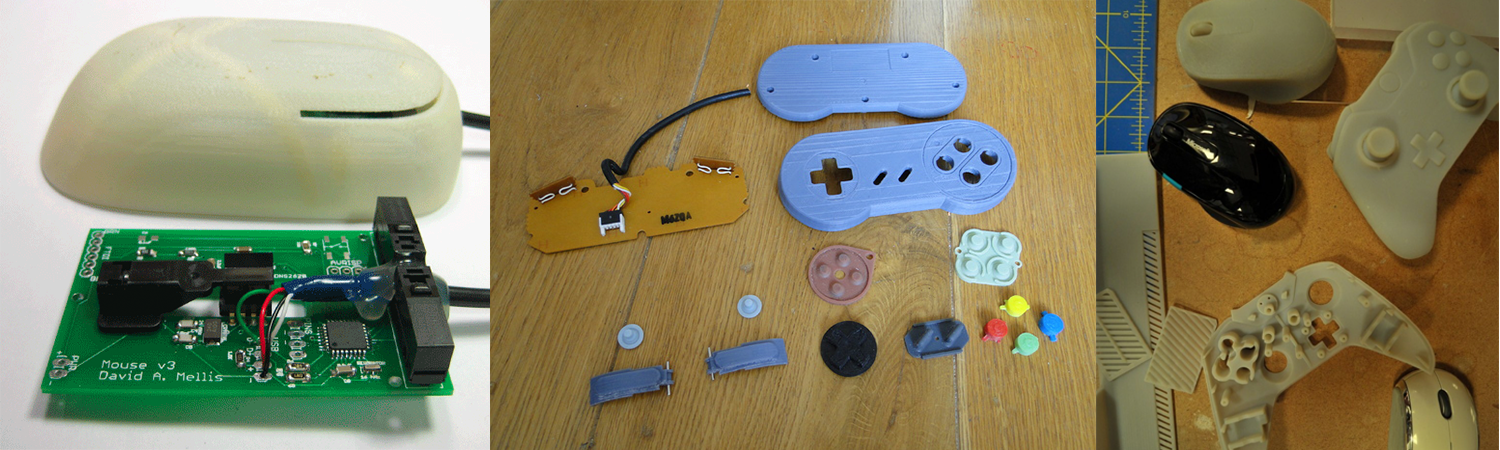
\includegraphics{figures/3dcases.png}
\caption{Makers use 3D printing to explore case form factors for interactive objects, like Dave Mellis's mouse (left) or Thingiverse author srepmub's game controller (center). Even professional designers like those at Microsoft use 3D printing for form-finding (right). However, this technique requires two separate processes: designing the case, then designing the functionality, typically in the form of circuitboards.}
\label{fig:3dcases}
\end{figure}

Existing research has developed electronic toolkits that lower the threshold of making physical prototypes interactive \cite{arduino,greenberg-phidgets}. However, such toolkits still require makers to manually assemble printed parts and sensors. Such assembly may also require significant changes to a 3D model (e.g., to add fasteners or split an enclosure into two half shells). Detailed electro-mechanical co-design is time-consuming and cumbersome and mismatched with the spirit of rapid prototyping. Alternatively, makers may instrument their  \emph{environments} with sensors \cite{akaoka-displayobjects,wilson-depthtouch} to add interactivity, but these approaches limit interactive testing to the lab in small, restricted areas.

\emph{We aim to uncover the most cost-effective, fast, and flexible ways of sensing rapid-prototyped input devices.} This suggests several requirements:
\begin{enumerate}
\item \textbf{cost-effective} : we substitute commodity sensors available in laptops and smartphones for custom electronic parts where possible. We focus on \emph{single-sensor} techniques, where sensing of multiple user inputs can be achieved by affixing a sensing apparatus to a single point, thereby reducing cost and assembly overhead.
\item \textbf{fast} : fabrication and assembly of senseable devices should not take significantly longer than comparable passive devices, and necessary digital modifications should be performed automatically when complex or be reduced to templates when simple.
\item \textbf{flexible} : the means of sensing a prototype object should not impose undue burden on the physical designs of that object. Sensing techniques should accommodate a wide variety of input types (e.g., buttons, sliders, and dials) and body types (e.g., convex, concave, 3D).
\end{enumerate}
We propose a novel way of ensuring these properties: users create digital design files, which our tools modify automatically based on knowledge of the sensing technique that will ultimately be used. Users then fabricate their modified models using digital fabrication machines. Because the physical models are precisely fabricated based on the digital design files, this process creates a \emph{link between the digital and physical models}. Post-fabrication, we leverage this link to inform sensor processing: this allows us to \emph{avoid training} and/or \emph{improve sensing} for the interactive prototype.

\section{Contributions}

This thesis explores the realm of physically prototyping tangible input devices using digital fabrication machines. We have built several prototype design and sensing systems designed to test different parts of the design space. Thus, this thesis makes the following contributions:

\begin{enumerate}
\item Fabbing to sense: a model and sensing co-design technique which uses knowledge of a particular sensing paradigm to automatically modify digital design files before fabrication, allowing improved or training-free sensing of the fabricated prototype. We offer three exemplars of this technique: Midas, Lamello, and Sauron.
\item Midas, a method for automatically generating custom capacitive touch sensors---cut from adhesive-backed conductive foil---by synthesizing sensor pads and routing connections from a high-level graphical specification:
%which allows a designer to author a high-level graphical specification of an object---and from that creates custom-shaped, flexible capacitive touch sensors by synthesizing sensor pads, auto-routing connections, and generating instructions for assembly and use: 
\begin{enumerate}
    \item a design tool using this method to enable users to to fabricate, program, and share touch-sensitive prototypes
    \item an evaluation demonstrating Midas’s expressivity and utility to designers
    \end{enumerate}
\item Lamello, a technique using passive plastic tine structures, 3D printed at interaction points and with predictable vibrational frequencies, to create passive tangible inputs sensed via audio:
%a technique which integrates algorithmically-generated audio-producing tine structures into movable components, creating passive tangible inputs---sensed by a microphone which classifies the tine-generated audio---that do not require training examples for accurate sensing:
\begin{enumerate}
    \item a design pipeline which predicts tine frequencies (and an evaluation that they can be accurately predicted) and senses user manipulation of components in real time
    \item a discussion of information encoding techniques useful for this technique, and a series of scripts to generate parts utilizing these encodings
    \end{enumerate}
\item Sauron, a design tool enabling users to rapidly turn 3D models of input devices into interactive 3D printed prototypes where a single camera senses input: %\valkyrie{this is the clearest description. modify others to be like this!}
\begin{enumerate}
    \item a method for tracking human input on physical components using a single camera placed inside a hollow object
    \item two algorithms for analyzing and modifying a 3D model’s internal geometry to increase the range of manipulations that can be detected by a single camera.
    \item an informal evaluation of our implementation of these techniques usable on models constructed in a professional CAD tool.
    \end{enumerate}
\end{enumerate}

\section{Dissertation Sketch}

This section presents a brief sketch of the structure of this dissertation by chapters.

This dissertation first investigates the capabilities of modern digital fabrication machines and discusses sensing techniques compatible with those capabilities. Second, a solid foundation of related work is laid out. We then discuss three instances of analysis and design tools that help users design, fabricate, assemble, and \emph{use} input devices sensed in a variety of ways; for each technique we demonstrate its flexibility for use in many types of input devices. Finally, we conclude with suggestions for future work.

\subsection{Fabrication \& Sensing (Chapter 2)}

This chapter explores modern digital fabrication machines and the properties that can be employed in objects they fabricate. We break down these properties, specifying which are inherent to materials, which are inherent to particular production processes, and which machines can currently realize objects with which properties.

Chapter 2 further discusses sensing techniques compatible with those capabilities, as well as what makes each technique promising. Again, we focus on techniques which require a single sensing apparatus attached to a single point on an object. For example, we discuss the potential combination of 3D printed conductive metal with Hall effect sensors; inducing a current through the object could create a magnetic field detectable by the sensors. This thesis ultimately selects a few points to further examine in this space, described in Chapters 4-6.

\subsection{Related Work (Chapter 3)}

We lay out the existing research landscape, describing which parts may have been overlooked and explaining which areas we explore in this thesis. In general, we draw heavily on work from four major traditions: simulation, sensing digitally-fabricated devices, modeling 3D objects, and creating prototypes.

\subsubsection{Simulation}
Simulation was one of the first hooks into fabrication research. Pre-fabrication simulation can ensure good coverage from robotic spray heads without occlusion from model features \cite{gursoz-noodles}, or account for deformities from specific printing processes \cite{hsu-numerical}. More recently, computer graphics researchers have leveraged pre-print simulation of multi-material printers to control post-print deformation behaviors \cite{bickel-deformation} and appearance \cite{lan-appearance}. We, too, perform pre-print simulation and optimization of 3D models, but for the purpose of creating \emph{interactive} objects.

\subsubsection{3D CAD Tools}
Many professional tools for 3D modeling exist \cite{solidworks, rhino}, and they serve their target users well. Researchers have made significant strides in inventing new styles of more accessible interactions for 3D modeling, for example by capturing users' hand-carving processes and convering them to toolpaths \cite{willis-interactive} or scanning, augmenting, and reproducing clay models \cite{savage-mmarks}. For the purposes of our investigations in this thesis, we created design tools to help author objects compatible with our sensing techniques: they are a complement to, rather than a replacement for, existing CAD tools research.

\subsubsection{Sensing Digitally-Fabricated Devices}
Sensing forms a key component of interactive devices, and thus has been significantly explored in the past. One common technique for sensing objects uses machine learning and guided manual training to detect interactions using sound \cite{ono-touchandactivate,laput-acoustruments}, capacitance \cite{sato-touche} or other signals. Our techniques focus on sensing done without machine learning, and often without any training at all. Inspired by ``Sensing Through Structure'' \cite{slyper-structure}, we design objects whose properties we know, which can inform how we sense them.

\subsubsection{Prototyping Tools}
Abundant research has examined questions around the types of prototypes that designers build in the course of designing a new object \cite{houde-prototypes}. Other work looks further into more facile ways of creating electronic and functional, for example using snap-together circuits \cite{littleBits, hartmann-dtools, villar-gadgeteer} or smart circuit substrates \cite{villar-voodooio}. One important limitation of these investigations is that they are limited to a constrained library of manufactured components: designers must make do with what they can buy. We conversely focus on customizable inputs that can be configured exactly as a designer wants them. Once an object is assembled, its functionality must be defined. We leverage techniques like programming by demonstration (PBD) \cite{myers-pbd, hartmann-dtools} to help users define their objects' interactivity.

%% \valkyrie{bjoern's these are really long... how long do they need to be??}

\subsection{Midas: Capacitive Sensing of Custom 2D Layouts (Chapter 4)}

Our first exploration examines fabrication of 2D conductive materials sensed capacitively. Midas pushes towards a world in which prototyping physical interactive devices is as easy as prototyping GUI devices. Midas's sensing is capacitive, building on the popular capacitive touch sensing built in to smart phones and other touch-screen devices, but it explores how to prototype touch-based interactions where input and output are \emph{not} co-located, as they are on touch screens. Designers are given a drag-and-drop authoring system to create capacitive touchpads on the surface of objects, and from these designs generates 2D design files for fabrication. These files can then be cut from a conductive material and sensed using an automatically-configured microcontroller board. Midas also offers support for programming the input devices designed via PBD and websockets.

\begin{figure}
\centering
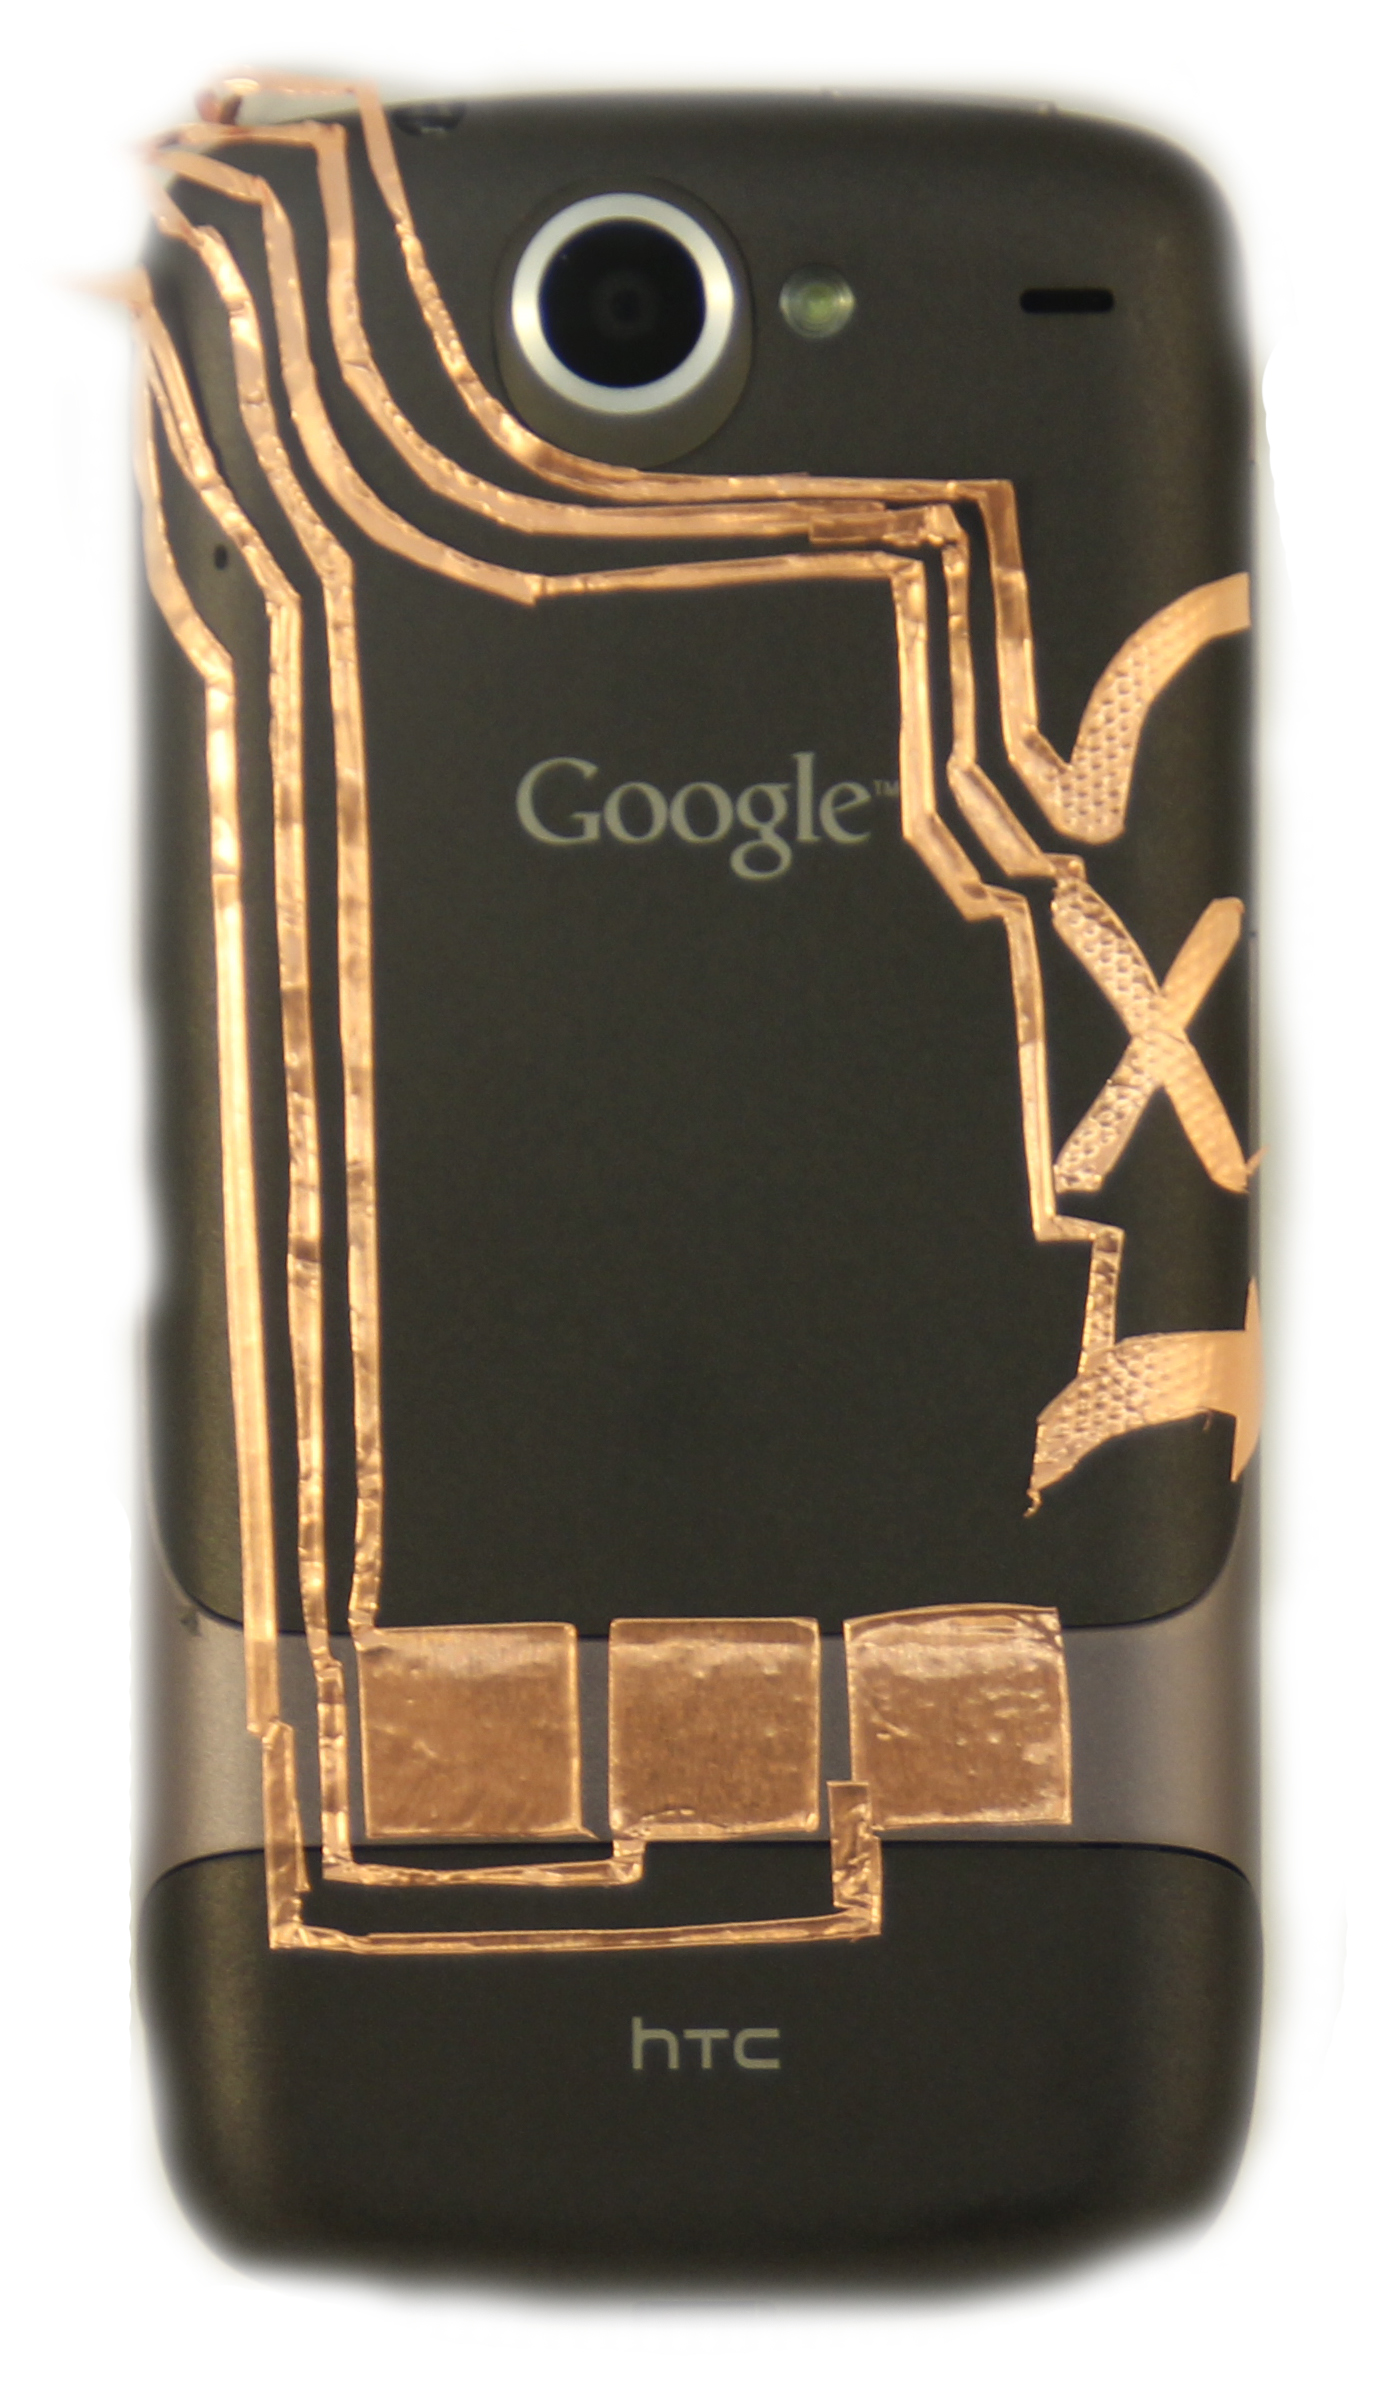
\includegraphics[width=2in]{figures/midas/midas-intro.jpg}
\caption{A Midas-generated interface with buttons for checking email mounted on the back of a smart phone.}
\label{fig:midas-intro}
\end{figure}

The advantages of capacitive sensing in this manner are numerous. It can be deployed on any flat, ruled, or developable object's surface (see Figure \ref{fig:midas-intro}). The sensors are cheap and easy to fabricate---whether on a vinyl cutter, using a circuitboard mill, or in inkjet printed conductive ink. Sensor assembly is \emph{fast}: users simply need to attach the sensor dongle's wires to their fabricated sensor pads (e.g., using tape).

In this chapter, we will detail Midas's implementation, as well as discussing possible uses, drawbacks of the current system, and work for the future.

\begin{figure}
\centering
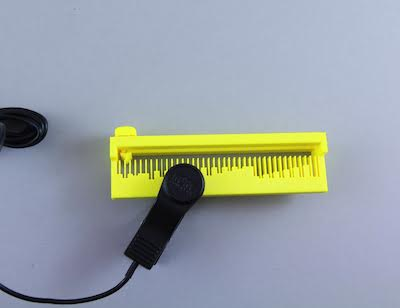
\includegraphics[width=3in]{figures/lamello/lamello-intro.jpeg}
\caption{A Lamello-based interface with a series of plastic tines on a slider, which can be classified by the attached contact microphone.}
\label{fig:lamello-intro}
\end{figure}

\subsection{Lamello: Acoustic Sensing of 2D/3D Mechanisms (Chapter 5)}

Second, this thesis dives into an examination of acoustic-based sensing for devices fabricated in 2D, 3D, or a combination. The Lamello project investigates the use of tine-like structures for repeatable and predictable audio frequency generation. These tines can be printed at interaction points (e.g., under the path of a human input slider) such that they are struck when a user manipulates input components. The mechanical vibrations created by striking the tines can be detected with a contact microphone and classified using frequency analysis (see Figure \ref{fig:lamello-intro}).

Leveraging uniform 2D lasercut or 3D printed plastics as sound-creating input devices offers flexibility to designers with different levels of access to fabrication machines. In addition, beyond Midas's offering of flat input surfaces activated by a simple touch, Lamello explores input mechanisms that users can push, slide, and turn. The technique of passive audio generation for sensing also opens up opportunities in the future Internet of Things: multiple unpowered Lamello-type input devices may be placed in the environment and sensed by a single microphone, perhaps located on a laptop or smartphone.

This chapter details our experiments confirming that our 3D-printed tine structures behave in predictable ways in spite of the non-uniform nature of the materials that comprise them. We also discuss, using several exemplars, techniques for integrating the tines into existing input component designs. Further, we describe information encoding principles for tine generation.

\subsection{Sauron: Vision-Based Sensing of 3D Printed Mechanisms (Chapter 6)}

Finally, we explore full 3D input devices sensed using computer vision. Sauron is a design and sensing toolkit for creating 3D printed input devices---which can include components like joysticks or dials---sensed with a single embedded camera. The Sauron tool makes automatic modifications to allow for this sensing, reconfiguring the \emph{interior} parts of the inputs and performing interference simulation (see Figure \ref{fig:sauron-intro}).

\begin{figure}[h]
\centering
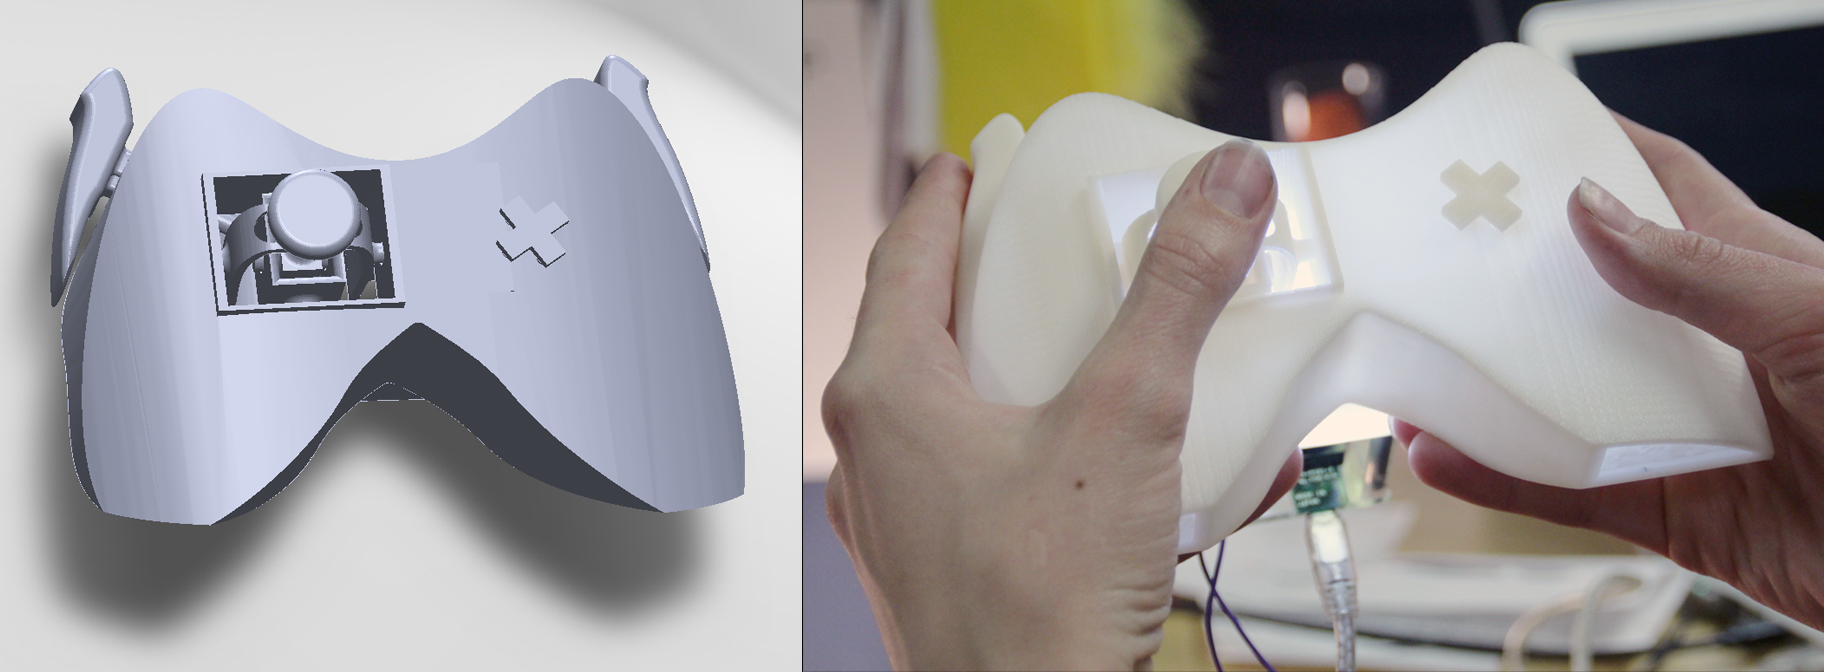
\includegraphics[width=4in]{figures/sauron/fig1-gamecontroller.jpg}
\caption{A Sauron-optimized game controller with a joystick, a direction pad, and several buttons.}
\label{fig:sauron-intro}
\end{figure}

Sauron's interfaces have additional flexibility over those for Midas or Lamello: they allow \emph{continuous} sensing of user input. They can be fabricated on any 3D printer which can generate support material, and the pre-fabrication simulation process relies only on geometry rather than any particular materials properties for its processing. %\valkyrie{not sure what else to put here...}

In this chapter we describe our implementation of Sauron as a plugin for a commercial CAD tool, as well as the vision sensing code we built. Finally, we elaborate on limitations of the current system and places we may improve it, as well as future work in the area.

\subsection{Conclusion \& Future Work (Chapter 7)}

The final piece of this thesis reviews the contributions described and re-evaluates assumptions made in the projects constituting its main chapters. Namely, our projects leverage a \emph{single fabrication machine} for creating \emph{one prototype} at a time, which is \emph{hand-optimized} by a designer and sensed by a \emph{single} sensor. Re-evaluating these leads to interesting pointers for future work in cooperation among fabrication machines, branching prototypes, machine-optimized prototype designs, and usage of combination sensors that can still be mounted at a single point.

\section{Statement of Multiple Authorship and Prior Publication}

The research presented in this dissertation was not undertaken by me alone. While I initiated
and led all projects described herein, I must acknowledge the contributions of my talented group of collaborators: without their efforts, this research could not have been realized in its current scope.

In particular, Midas's routing features were implemented by Xiaohan Zhang, and the video was created by Lora Oehlberg. Andrew Head performed much debugging and audio testing on the Lamello project, and that project benefited from the wisdom of my collaborators Dan Goldman (who provided the initial idea), Gautham Mysore, and Wilmot Li at Adobe. Sauron's computer vision was implemented by Colin Chang, and many thanks are due Mark Oehlberg for assisting in the creation of the necessary circuitboards for that project.

My advisor, Bj\"orn Hartmann, provided invaluable advice and guidance on all projects detailed in this document.

This dissertation is partially based on papers previously published in ACM conference proceedings; I am the primary author on all publications. In particular, Midas was published at UIST 2012 \cite{savage-midas}; Lamello at CHI 2014 \cite{savage-lamello}; and Sauron at UIST 2013 \cite{savage-sauron}.
\chapter{Fabrication \& Sensing of Input Devices}


\begin{quote}
One of the criticisms we get is, 'Does the world need more plastic crap?' But you have to look beyond the plastic crap, to the design, to the experience, to the empowering nature of [digital fabrication] and the community.

--- Bre Pettis
\end{quote}

This chapter outlines the multitude of digital fabrication techniques currently available, as well as potential characteristics of the artifacts that each process can create. We then align these properties to sensing techniques, describing a space of possible geometry/sensing links for input device design and fabrication. \valkyrie{I would add a little bit of detail here. What does ''link" mean? Just another sentence or two that spells out more explicitly that we want to fabricate objects with properties which can in turn be sensed. Maybe even give an example in here to make this concrete: "For example, different processes can create tine structures (cantilevered beams). Those beams, when struck, vibrate at frequencies determined by their geometry, which can be sensed with a microphone."}

\valkyrie{Hmm, writing this made me realize that maybe we need to describe more than just the pairing between fab characteristics and sensors? Maybe: 1) user action 2) mechanism 3)material characteristic 4) sensable change from coupling 1 to 2 5) sensor selection. You do this at the very end of this chapter. Maybe we want to bring this into the intro somehow?
For Midas: 
1) touch 2) none 3) conductivity 4) capacitance 5) capacitive touch chip
For Sauron:
1) physical movement (push/slide/rotate); 2) 3d printed mechanism 3) rigidity, color 4) visual motion 5) camera
For LAmello
1) physical movement 2) plucking mechanism 3) controlled tine geometry 4) vibration 5) microphone}

\section{Definitions}

First, we briefly define words and machines that will be discussed in this chapter and the remainder of the thesis.

\emph{additive fabrication} : in additive fabrication, material is deposited and a shape is built up.

\emph{subtractive fabrication} : a subtractive fabrication process removes material to create a form. Excess material may be reused in another project or discarded.

\emph{3D printer} : a 3D printer is one of a class of machines that additively create a three-dimenstional model from one or more materials.

\emph{FFF} : FFF (fused-filament fabrication) 3D printers lay down material by melting and depositing a filament in a precise pattern.

\emph{model material} : model material is the substrate that the final object is made from

\emph{support material} : many modern 3D printers are capable of laying two types of materials, model material and a secondary, sacrificial material that can support overhangs in the model while printing, then be removed.

\emph{SLA} : SLA (stereolithography) printers use a bath of UV-curable polymer and a controllable UV laser. The laser "draws" each layer on the polymer, causing photopolymerization where it strikes. Excess material is simply poured out for reuse.

\emph{SLS} : SLS (selective laser sintering) 3D printers contain a bed of material (e.g., metal powder) which is compacted and formed into a solid mass of material by heat and/or pressure without melting to the point of liquefaction. Excess material can be brushed off and reused.

\emph{Polyjet} : Polyjet printers have print heads similar to those of inkjet printers which sweep across the build area depositing material. Following the printer head is a UV light, which cures deposited material droplets.

\emph{vinyl cutter} : a vinyl cutter subtractively processes 2D materials with a 2-axis knife blade, cutting patterns into them. Vinyl cutters are typically used for thin, flexible materials.

\emph{laser cutter} : a laser cutter has a 2-axis laser for processing flat materials. Laser cutters can cut or engrave into materials, and are often used for rigid materials $1</4$ inch thick. Some have rotary attachments for etching on circular surfaces like the outside of a glass.

\emph{CNC router} : a CNC router uses a 3-axis rotary mill to cut through thick, rigid materials, like wood or certain metals. Some CNC routers are portable and can attach to many materials, while some are stationary with beds into which material is loaded.

\emph{CNC mill} : a CNC mill is a multi-axis machine which subtractively creates a 3D shape from a block of material, usually metal or wood.

\section{Digital Fabrication}

Digital fabrication machines are those which can take as input a digital design file, in 2D, 2.5D, or 3D, and output a physical realization of that design. A design created in a computer-aided design (CAD) tool is processed by a computer-aided manufacturing (CAM) tool to create machine instructions to generate the object. This workflow stands in contrast to traditional crafting techniques (which do not require machine code) as well as manufacturing techniques (which require ``tooling'' for each design created). The true power of digital fabrication lies in its ability to create unique objects with each machine run \emph{without} the extensive setup and tooling necessary to change the product created by, for example, an injection moulding machine. This comes with the blessing and curse that each instance of an object costs as much to manufacture as the one before it, but allows for variations between instances without additional cost. For example, even makers can now create custom 3D printed replacement joints and prosthetics that fit particular bodies, e.g., a new hand for a young girl who wants to do monkey bars \cite{myers-sophie}.

The joint interests of industry, academia, and hobbyist makers have led to a flourishing ecosystem of digital fabrication and rapid prototyping (RP) machines. These machines describe a continuum from simple vinyl cutters that can subtractively create 2-dimensional stickers to sophisticated multi-material 3D printers that can create multicolor and conductive designs where the designer has full 3D control over the external and internal geometry of object. These machines allow their manufactured products to achieve various material and structural properties. We examine materials properties of common digital fabrication inputs (see Figure \ref{table:fab-properties}), as well as the machines that can process them and the compositional properties they make possible (see Figure \ref{table:materials-machines}).

\begin{figure}
\centering
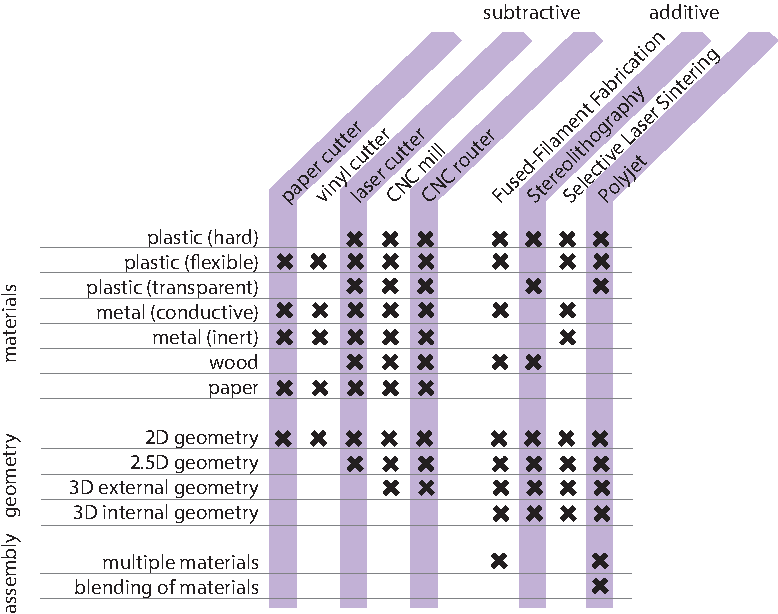
\includegraphics[width=3in]{figures/fab-properties.pdf}
\caption{The most common materials processed by digital fabrication machines, including plastic and wood, have wildly different realizable characteristics.}
\label{table:fab-properties}
\end{figure}

\begin{figure}
\centering
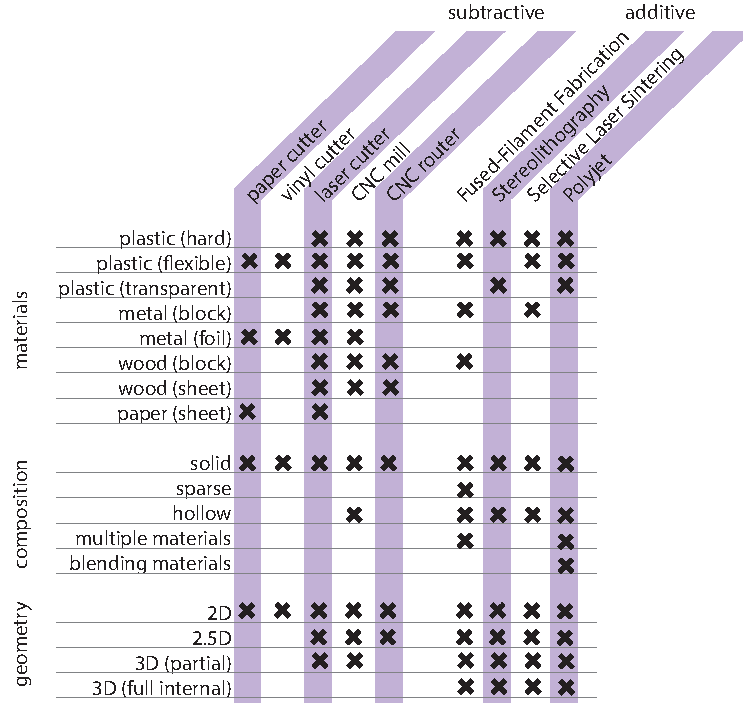
\includegraphics[width=5in]{figures/materials-machines.pdf}
\caption{Additive and subtractive RP machines each have their own sweet spots of operation. Subtractive tools can process more types of materials, but additive ones offer more compositional flexibility.}
\label{table:materials-machines}
\end{figure}

\subsection{Geometry Fabrication}

Digital fabrication machines can support any complexity of geometry, from 2D images on paper (as an inkjet printer produces) to 3D projections of 4D objects (like Shapeways's Klein bottles printed in steel) (see Figure \ref{fig:range}). We describe the possibilities for the various geometries, as well as machines that could produce them. Note that we list machines at the edge of their range: for example, a CNC mill (listed under 3D external) can also make 2.5D or 2D objects.

\begin{figure}
\centering
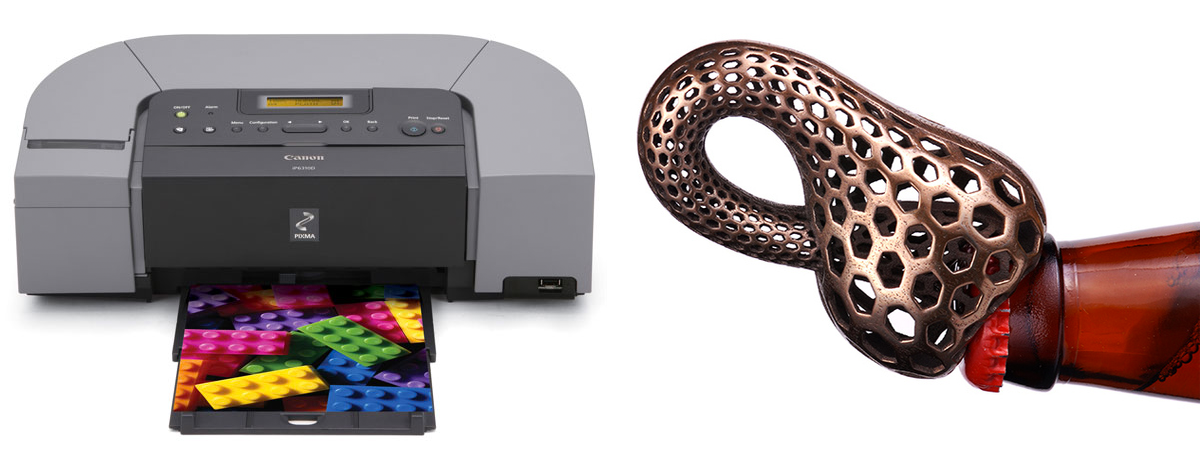
\includegraphics[width=4in]{figures/range.png}
\caption{The range of objects produceable via digital fabrication is huge: from 2D images on paper (left, from Amazon), to 3D projections of 4D objects (right, from Bathsheba on Shapeways).}
\label{fig:range}
\end{figure}

\subsubsection{2D geometry}

2D geometry lies flat on a surface, but can manifest as an image printed on paper, a sticker cut from vinyl, or a barcode engraved on granite. Machines that support 2D geometry fabrication include vinyl and paper cutters, as well as inkjet printers.

\subsubsection{2.5D geometry}

A slight jump from 2D is 2.5D: a 2D shape with additional \emph{depth} information. The canonical machines to create 2.5 objects are 3-axis CNC routers, which mill away material from the surface and can take multiple passes for deeper features.

\subsubsection{3D external geometry}

Features like overhangs can be challenging to mill using a 2.5D machine, as subtractive techniques require that the machine tool has unobstructed access to the surface to be milled. Creating such features on a 2.5D machine may require reorienting an object several times. Some machines are capable of creating arbitrary 3D external geometry, including overhangs, without manual reorientation of a part. This is can be accomplished by machines that use both a model material and a sacrificial support material: combining the two materials permits overhangs that may not be possible using only a single material. However, removal of this support material can be challenging, depending on the process used. (See \cite{savage-sot} for a more complete treatment of support material and removal techniques.) 3D printers can produce overhang geometry by laying support material as a part of each 2D object slice, and 5-axis CNC mills can produce overhangs via automatic object reorientation.

\subsubsection{3D internal geometry}

Full control over internal geometry can only be executed via additive manufacturing, and it allows for designed cavities, mechanisms, textures, and more on the interior of objects manufactured in a single pass. Again, this is typically executed by machines that lay sacrificial support material.

\subsection{Materials and Properties}

Beyond geometric properties, the types of materials that can be processed using the various additive and subtractive RP machines is equally broad. Each material lends itself to certain types of manipulations, and different materials may be more easily formed by different machines.

\valkyrie{I wonder if properties would be the better top-level organizing principle, rather than materials:
so: Appearance: opaque-translucent-transparent
Appearance: color-no color
Rigidity: rigid-flexible
Conductivity: isolator-resistor-conductor ?
Material fill : solid-sparse-hollow
Then you could have process x material gives rise to certain properties. add color}

\subsubsection{Plastic (hard)}

Hard plastics---including thermoplastics like acrylonitrile butadiene styrene (more commonly known as ABS) and polylactic acid (known as PLA)---are the materials du jour in the maker community. They come in the form of heatable, extrudable filaments for FFF machines (e.g., Makerbot, Printrbot, Reprap, uPrint). Hard plastics can also be additively processed with other 3D printing techniques, for example photocure plastics in polyjet machines (ABS-like and Vero series for Objet machines) and SLA machines (methacrylates in Form1), or thermoset plastics like epoxy in research systems (e.g., Harvard's system \cite{compton-epoxy}).

Hard plastics can also be subtractively processed through milling and laser cutting, although many plastics are unsafe for laser vaporization (e.g., ABS plastic emits chlorine gas when lasercut).

\subsubsection{Plastic (flexible)}

Flexible plastics are less common than hard ones, though there are some notable materials here: thermoplastic polyurethane (sold as Ninjaflex) is a filament-style flexible material for use in FFF machines, and some polyjet machines likewise have support for flexible plastics (e.g., Tango series for Objet).

Subtractive processing for flexible plastics is possible, though may be more challenging due to different shear parameters than stiffer materials. PVC plastic in the form of vinyl sheets can be cut to shape with a vinyl cutter.

\subsubsection{Plastic (transparent)}

Transparent plastics are not yet available for most maker-class machines, though many SLA-processed resins are optically translucent and polyjet machines offer optically transparent plastics (e.g., VeroClear for Objet). Laser cutters are suitable for processing sheets of transparent acrylic, as well.

\subsubsection{Metal (conductive)}

Conductive metal is relatively simple to process subtractively (e.g., milling circuitboards on a CNC router), even by vinyl cutters which can cut thin metal foils. Certain conductive metals, e.g., steel, can be directly laser-sintered in a high-heat process. Conductive-impregnated filaments for FFF machines do exist in limited use, but they are typically based on graphene (carbon) rather than metals. The new Voxel8 FFF 3D printer \cite{voxel8} uses a silver-based material for conductive purposes.

\subsubsection{Metal (inert)}

Inert metals are processed in essentially the same ways as conductive metals, although they have not been engineered for use in FFF filaments.

\subsubsection{Wood}

Wood-type materials are most commonly subtractively processed (e.g., by CNC routing). Newer processes are available to add wood in the form of sawdust to FFF-compatible filaments (e.g., woodfill by colorfabb), and also to laser sinter with wood chips \cite{materialise-wood}.

\subsubsection{Paper}

Paper is trivially subtractively processed. None of the four main 3D printing methods can use paper-based materials, though one subtractive/additive method uses stacks of cut paper to create 3D paper models (e.g., MCor IRIS).

\subsection{Assembly Characteristics}

\valkyrie{This paragraph is very abstract. I’m not sure what to take away from it.}

Additive digital fabrication methods offer significant freedom in terms of assembly methods. Many types of printers can use multiple materials for the same part, and even blend them. This allows for fabricating parts of multiple colors or shore (hardness/softness) values, or simply creating parts which are pre-assembled and interlocked after support material is removed. 

\section{Single-Sensor Sensing Techniques}

One key research area in Human Computer Interaction is designing new techniques and algorithms to help computers accept human input. Thus, while many of the input techniques here could be used in, for example, machine-to-machine communication, we describe how a person's actions might create a usable control signal.

\valkyrie{repeat single-sensor motivation} A ``single sensor'' can take many forms, ranging from a humble switch which opens and closes to a high-speed video camera which captures 2D visual information at 1000Hz to an accelerometer measuring G-forces in 3 directions.
%\valkyrie{Card, et al., provide an analysis of the space of input devices based on what is sensed: position, $\Delta$position, angle, $\Delta$angle, force, $\Delta$force, torque, and $\Delta$torque \cite{card-input}. We use this to frame our discussion, but include additional senseable aspects: identity (of a user), bend/$\Delta$bend, and ???. We could also include, for example, \emph{intent}, which is the input of NLP voice systems like Siri, however these types of non-physical input are challenging to conceive of as a part of a physical input device and we therefore ignore them for now.}
We organize our discussion around five categories of common sensors: contact, non-contact, electrical, environmental, and biological. In these five categories, we discuss thirty common varieties of sensors, like capacitance sensors, hall effect sensors, voltage sensors, temperature sensors, and pulse sensors.

\valkyrie{The major categories in the Modern Sensor Handbook are:
* occupancy and motion
* position, displacement and level
* velocity and acceleration
* force, strain and tactile
* pressure
* flow
* acoustic
* humidity/moisture
* light detectors
* radiation detectors
* temperature
* chemical sensors}

\valkyrie{The physical effects that are the basis of sensors include: capacitance, magnetism, induction, resistance, piezoelectric effect, pyroelectric effect, hall effect, thermoelectric effect, ...}

\subsection{Contact sensors}

Contact sensors are mainly used either to sense contact with an object (in the case of switches, capacitance, flex, or force sensing) or used while in contact with an object to sense other forces on it (as in load sensors, accelerometers, and gyroscopes). This kind of sensor can directly sense physical human input.

\subsection{Non-contact sensors}

Non-contact sensors, like the contact variety, can directly sense physical human input. They can, however, do so without being in contact with the human or the input device being sensed. Non-contact sensors rely on waves (e.g., visible for cameras, audible for microphones, radio for RFID) or fields (e.g., magnetic for hall effect) to sense interactions. 

\subsection{Electrical sensors}

Electrically-based sensors like volt-meters and potentiometers can be used as tools for internal monitoring of a circuit, but are also able to sense human input. A potentiometer attached to a knob, for example, will change its resistance value as a user manipulates the knob.

\subsection{Environmental sensors}

Environmental sensors, like pressure and altitude sensors, are generally used to sense ambient details, as opposed to human input. However, certain ambient details can be modified by human presence or activity: for example, human users can output sweat senseable via humidity sensors, and human presence may raise the local temperature of a area.

\subsection{Biological sensors}

Human bodies perform several semi-controllable processes: hearts beat, brains think, etc. Biological sensors detect these processes. They can be used for input by humans, but the user may require some training to be competent at creating distinct signals.

\section{Promising Overlaps}

The spaces of both machines and sensors are vast, so we describe some ways to think about combining them to actually fabricate sensing objects.

\begin{figure}
\begin{adjustbox}{addcode={\begin{minipage}{\width}}{\caption{%
      Lining up the possibilities of fabricatable properties with sensor types, we can see several areas that are promising for further exploration. We also identify pairings that have been explored previously, as well as pairings explored in this thesis. 1. Capricate \cite{schmitz-capricate}, 2. Flexibend \cite{chien-flexibend}, 3. Stane \cite{murray-smith-stane}, 4. Printed Optics \cite{willis-printedoptics}, 5a. Design by physical composition \cite{doering-composition}, 5b. Dynamic latex buttons \cite{harrison-buttons}, 6. Depth camera as touch sensor \cite{wilson-depthtouch}, 7. Pressure-sensing robot skins \cite{slyper-pressure}.
      }\end{minipage}},rotate=90,center}
      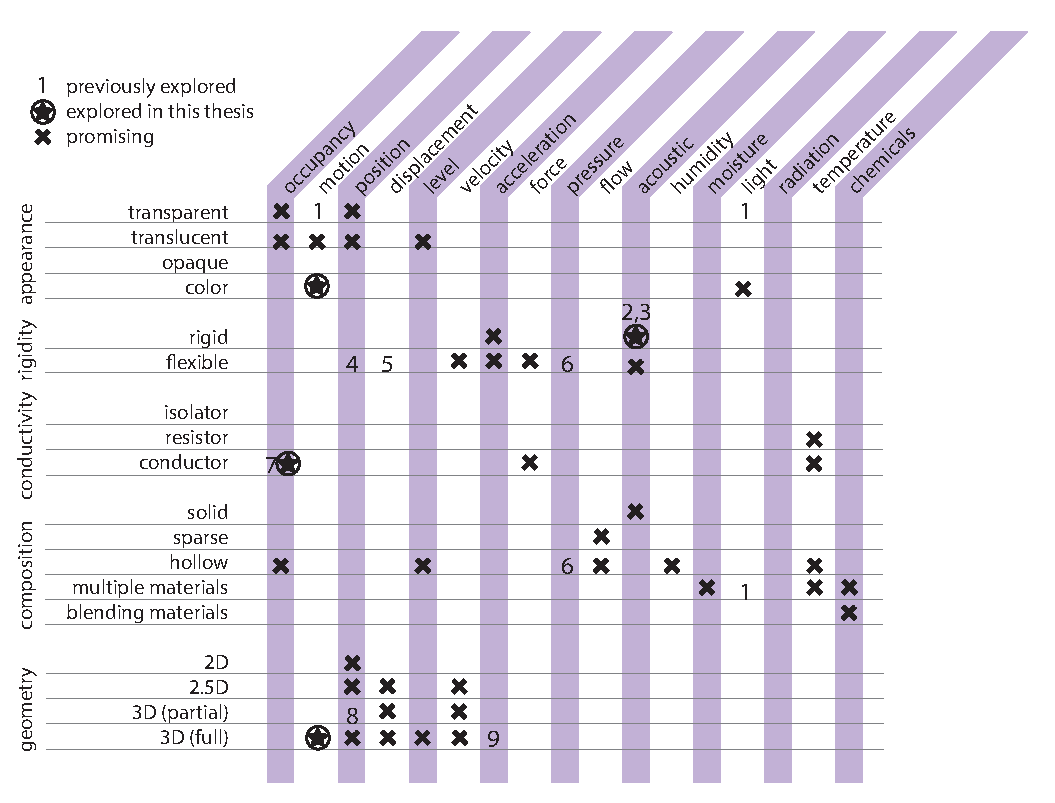
\includegraphics[scale=.75]{figures/sensing-fab.pdf}%
  \end{adjustbox}
\label{fig:sensing-fab}
\end{figure}

\subsection{Principles}
    
    Several principles guide our selections. Namely,
    \begin{itemize}
      \item for materials: \begin{itemize}
        \item the material ideally conducts (but at least does not insulate) the signal to be passed. For example, metal conducts electricity, and so is compatible with electrical sensing; paper conducts moisture, and thus could be used with humidity sensing.%; pulse can be sensed optically, so clear material may be compatible with pulse sensing.
        \item a user's manipulating the material should generate a control signal senseable using the given sensor. For example, bending a flexible plastic generates a signal detectable by a flex sensor. %\valkyrie{actually different from above?. yes.}
        \end{itemize}
      
      \item for geometry: \begin{itemize}
        \item geometry should work with the sensing abilities of a given technology. For example, an object with a solid core would not allow fluids to sense for particulate sensing; allowing 3D internal geometry would make this sensing possible.
        \item geometry needs to make it possible for a given type of signal to reach every part of an object without collision. For example, a camera inside a 3D object may require geometry modifications  or mirrors to see around corners. \valkyrie{still chewing on this one...}
        \end{itemize}
      
      \item for assembly characteristics: assembly characteristics of an object may be necessary in combination with particular materials properties to get additional sensing. For example, blending stiff and flexible plastics may allow for more unique degrees of sensing with a flex sensor. \valkyrie{still not clear after previous discussion of assembly techniques}
      
      %\item for sensors: to avoid complex machine learning, sensors should measure phenomena which can be mathematically modeled from digital design files. For example, the range from an ultrasonic rangefinder to a moving slider may be easier to model than the force generated by a user flexing a part with a Shore value of 35. \valkyrie{do we need this section? basically all the other sections reference sensor compatibility anyway.} \valkyrie{realistically, a caveat is that I know more about contact/non-contact/electrical sensors than I do about the other things. they are more commonly used in HCI as far as I'm aware, and maybe I just don't have the brain bendability to identify how they could be effectively leveraged using fab.}
    \end{itemize}
    
    These principles give rise to the \textbf{x}s marked in Figure \ref{fig:sensing-fab}.
    
\subsection{The Most Promising Overlaps}

    \valkyrie{choose a few things outside this thesis that we think are the best places to look next. blendable flexy materials + FSR. print electromagnets with conductive material, sense motion with gausssense (sensor block powers magnet channels??)}
    
\subsection{Overlaps Discussed in this Thesis}

    \subsubsection{Conductive Metal + 2D Geometry + Capacitive Sensor}
    
    Chapter 4 describes Midas, a technique for creating custom capacitive touchpads CNC cut from adhesive copper foil. These can be affixed to everyday objects and sensed using a single capacitive touch controller.
    
    \subsubsection{Hard Plastic + 2D/3D Geometry + Microphone}
    
    Chapter 5 describes Lamello, a technique for creating tines from hard plastic; when struck each tine vibrates at a characteristic frequency which can be classified using a microphone.
    
    \subsubsection{3D Internal Geometry + Camera}
    
    Chapter 6 describes Sauron, a technique leveraging arbitrary internal geometries to create mechanical input devices that can be sensed by a single embedded camera.
\chapter{Related Work}

\begin{quote}
If I have seen further, it is only by standing upon the shoulders of giants.

--- Isaac Newton
\end{quote}

Situating this thesis in the realm of prior work, we draw heavily on work from four major traditions: simulation, sensing, 3D modeling, and prototyping tools.

\subsection{Simulation}

    The simulation community was one of the first to rally around digital fabrication: they have delved extensively into digital simulation of materials and behaviors, and the advent of hyper-precise 3D printers like the Objet Connex line\footnote{At time of publication, the Connex3 allowed for XY resoltion of $600$dpi, Z resolution of $1600$dpi, and accuracy of 20-85 microns. \url{http://www.stratasys.com/~/media/Main/Files/Machine_Spec_Sheets/PSS_PJ_Connex3.ashx}} allowed for a variety of real-world manifestations of these simulations.
    
    Mathematical simulation for structural analysis existed before digital fabrication, e.g. \cite{fleury-optimization}, and supported CNC machining. Some of the very earliest work on fabrication-related simulation focused on optimizing toolpaths, for example to ensure good coverage from robotic spray heads without occlusion from model features \cite{gursoz-noodles}. Other early work examined and accounted for deformities in models produced using different 3D printing technologies \cite{brown-simulate,hsu-numerical}, or ensuring printability of 3D models \cite{barequet-gaps,bohn-shellclosure}. More recently, visual simulation (i.e., graphics) researchers have investigated modeling and fabrication of deformation behavior \cite{bickel-deformation}, as well as subsurface scattering \cite{hasan-subsurface} and subsurface reflectance \cite{weyrich-reflectance}. Precision fabrication machines allow for creating tiny structural elements that can contribute to an object's overall appearance \cite{lan-appearance}.
    
    Higher-level optimization strategies can yield models with voids inside to ensure balance after fabrication \cite{prevost-makeitstand}, or musical instruments which have specific pitches after fabrication \cite{umetani-metallophone}. Another system can take motion capture sequences and translate them into fabricatable mechanical automata that perform the same motions \cite{ceylan-automata}.
    
    The actual fabrication process can also be improved with recent work in graphics. For example, linking knowledge of the layered manufacturing technique employed by FFF machines (described in Chapter 2) to a 3D model can help ensure that it will not break under force \cite{umetani-strength}, or that fabrication will produce minimal waste \cite{schmidt-support}. Properties of materials post-print can inform the design of automatically-inferred joints for poseable characters \cite{bacher-posable,cali-articulated}.
    
    This thesis will draw on the same theme of pre-fabrication simulation of materials and models. Certain types of sensing necessitate guaranteeing that a prototype will have specific material properties, however our focus does not end with the fabricated object itself. We use information from the model to inform our sensing techniques and to develop interactive prototypes.
    
\subsection{3D CAD Tools}
    Tools for 3D modeling are becoming more useful and usable as 3D printers become more accessible. Powerful industrial modeling tools, like SolidWorks \cite{solidworks}, AutoCAD \cite{autocad}, ProEngineer \cite{proe}, and Rhino \cite{rhino}, have existed for years and served industrial designers and professional engineers very well. Makers find lower-threshold, lower-ceiling tools like Meshmixer \cite{schmidt-meshmixer} suitable for their needs. However, research has investigated more accessible ways of modeling objects.
    
    Creating an object that fits with existing hardware has been explored using Kinect-based scans of objects \emph{in situ} \cite{molyneaux-kinectfusion, weichel-mixfab} or photographs \cite{lau-modeling}, or intelligent capture of object dimensions with measuring tapes \cite{lee-handscape,weichel-spata}. Other work has explored tangible manipulation of building blocks \cite{anderson-tangible, gupta-duplotrack} or clay models \cite{savage-mmarks}. 3D models can even be created from sketches, by exploiting prior knowledge of post-fabrication material properties \cite{mori-plushie, saul-sketchchair}. Our work touches on 3D modeling, however we focus on augmenting existing 3D models with sensing rather than creating new ones from scratch.
    
    Other research explores capturing a designer's toolpath and creating a model and/or final artifact by automatically tidying it up \cite{willis-interactive, mueller-constructable, mueller-laserorigami}, or conversely \emph{directing} a toolpath using information from a 3D model and enabling a dialogue between user, tool, and model \cite{zoran-freed}. Once a designer creates an initial model, other tools allow modifying it tangibly, for example by letting the user sketch modifications on a printed version \cite{song-modelcraft-tochi}. We similarly link object geometry to its physical form, however we pursue this link for sensing purposes rather than for form finding.
    
    Sensing modules can be the primary driver of an object's form factor, for example by allowing designers to drag the modules around digitally and re-forming a shape that will hold them all \cite{weichel-enclosed}. This technique could be useful as an add-on for our tools, but we focus on sensing rather than authoring 3D case forms. Pipe structures for joining sensors to microcontroller boards can allow for additional flexibility in design \cite{savage-sot}, however this requires that the designer has intimate knowledge of the sensing techniques to be used. Our tools build in knowledge of the sensing paradigm, relieving that burden from designers and allowing additional redesign flexibility versus one-off, hand-created sensor routings \cite{navarrette-gps, park-microchannels}.

\subsection{Sensing Techniques}

    %\valkyrie{not all of these are for fabbed objects, but a slightly broader swath of sensing techniques definitely needs to be discussed here. segmenting into fabbed vs. not doesn't really draw a bright line of any kind, though, so... how to structure this part?}
    Research has likewise investigated a variety of ways for sensing manually- and digitally-fabricated devices, ranging from switches that close when a flexible object is bent \cite{slyper-structure} to audio frequencies swept through fabricated flutes \cite{laput-acoustruments}.

    \subsubsection{Using machine learning}
        Machine learning provides power and nuance to sensing tasks. By sweeping electrical frequencies through a conductive material (e.g., water), machine learning can detect if a user touches it with a finger versus with two fingers \cite{sato-touche}, or using audio in a similar way can detect palm versus fingertip interactions with objects \cite{ono-touchandactivate}. The acceleration profiles of scratching noises can be detected as gestures \cite{harrison-scratchinput}, and scratching noises along ridges can reveal whether a user is rubbing an object clockwise or counterclockwise \cite{murray-smith-stane}. Simple camera-based and depth-camera-based sensing can likewise be trained to detect user interactions  \cite{fails-crayons,holman-sketchspace,klemmer-papiermache,macintyre-DART}.
        
        Even more subtle interactions can be captured, for example by using continuous interpolation of signatures. This has been applied to sound swept through 3D printed flute-like tubes \cite{laput-acoustruments} to determine position continuously along sliders.
        
        However, employing machine learning requires training each gesture to be sensed. In addition, it requires training each \emph{combination} of gestures to be sensed, as swept sound or capacitance signatures may not combine linearly when gestures are performed contemporaneously. Our work eschews this complication: since we link geometry to sensing, we exploit this link to allow training-free sensing and/or improve our chances of sensing a user's interactions correctly.
    
    \subsubsection{Without machine learning}
        Other explorations have led to clever ways of avoiding the post-fabrication training necessary to use machine learning for sensing. For flexible objects, this can come in the form of internal switches designed to close when cast-silicone objects are manipulated in certain ways \cite{slyper-structure}, or as conductive material within microchannels whose resistance changes when stretched or bent \cite{majidi-curvature, park-microchannels}. Time-domain reflectometry, i.e., sending an electrical pulse through a wire and timing how long it takes to reflect back, can likewise detect user interaction with flexible objects \cite{wimmer-tdr}, as can adhesive sensing tape \cite{holman-tactiletape}. These techniques do not employ digital fabrication: they are hand-fabricated and -tuned. Because we digitally fabricate our artifacts, we can generate knowledge of geometry automatically. Digitally fabricated soft objects can have stretchable electronics embedded afterwards \cite{yao-pneui}, or be sensed using computer vision and barometric pressure \cite{harrison-buttons, slyper-pressure}; however, since these objects do not use knowledge of their interactive pieces, they cannot exploit the geometry-sensing link that we use for our work. Similarly, Olberding, et al., created a sensor that is maximally robust to post-fabrication user modification \cite{olberding-cuttable}. Again, this technique does not exploit the link between an object's geometry and its fabricated form to improve sensing.
        
        Identity can be embedded in fabricated objects' surface textures (intended for scratching) \cite{harrison-acoustic}; indeed identity can also be recorded in invisible chambers \emph{inside} an object for later high-frequency imaging \cite{willis-infrastructs}. These projects use knowledge of the fabricated, embedded identity tags to ``train'' their sensing, however they can only detect an object's identity and not how a user is interacting with it.
        
        Actual user interaction with digitally fabricated objects has been explored, as well, most notably by Willis, et al. Printed Optics allows for sensing fabricated mechanisms (like sliders and buttons) via light shining through tiny channels embedded in a print \cite{willis-printedoptics}. This work inspired our own, though Printed Optics does not offer a design tool or a way of providing this sensing without extensive hand-programming.

\subsection{Prototyping Tools}

    Our investigations in this thesis are ultimately looking at techniques for prototyping. There are many different types of prototypes: typically they are split into role, look-and-feel, and implementation \cite{houde-prototypes}. Within each of these types of prototype, there are opportunities to explore high-fidelity prototypes and low-fidelity prototypes. Our work seeks to help with high-fidelity look-and-feel and role prototypes; we recognize that our sensing techniques have some drawbacks as tools for final implementation (for example, the processing time required to recognize interactions using computer vision or audio).
    
    Other research has investigated easing this type of physical functionality exploration, often through the creation of toolkits that help users create interactive prototypes quickly. On the low-fidelity end, simple pushpins and copper tape can create circuitry for testing with cardboard mockups \cite{hudson-boxes}, or the TUIs can be ``sketched'' using augmented reality tools \cite{nam-sketchingtuis}. Another simple solution is attaching an accelerometer to an object and using its output to detect interactions \cite{hook-making}. More sophisticated toolkits may include multi-purpose programmable microcontrollers \cite{arduino}, or even be designed for prototyping interactive devices on cloth \cite{buechley-lilypad}. Designers can have extra freedom with placing electronics when a board becomes a smart substrate that interlinks them automatically \cite{villar-voodooio}, or can use snap-together sensing and actuation modules \cite{avrahami-switcharoo, greenberg-phidgets, lee-calder} that could be programmed in a visual language \cite{villar-gadgeteer}. These techniques have several important limitations: most importantly, they \emph{constrain exploration}: if a user wishes to include a 3-inch slider in his design, but the kit only offers a 2-inch slider or a 5-inch slider, he has to make due. Our work's use of digital fabrication for sensor creation gives users this flexibility in design exploration, without tying them to pre-defined form factors.
    
    Circuitry, and thus any existing electronics, can be integrated directly into a 3D printed object by laying down conductive material \cite{sells-reprap,voxel8,sarik-tracebrush}, or by leaving voids to be filled with conductive material post-print \cite{savage-sot}; this still constrains designers to what already exists. Techniques like adding stick-on sensors or sensing tags \cite{maynes-aminzade-eyepatch,yeo-stickear} can mitigate this challenge, however they lead to one-off prototypes: with digital fabrication, designers can create a design, test it, then modify it digitally to create an improved design; they can even share it with coworkers without rebuilding it by hand each time. A more general purpose sensing \emph{core} can be added to new prototypes, necessitating that only the body of the design change each time \cite{doering-composition}: we build on this idea and leverage our knowledge of an object's geometry to improve it.
    
    We also examine another important question: how is functionality defined in interactive prototypes? Software can be automated using screenshots as in Sikuli \cite{yeh-sikuli}, or with visual ``block''-based programming languages that are accessible to even children \cite{resnick-scratch}. Programming by demonstration can also aid novices in developing interactive applications with sensor components \cite{hartmann-dtools}, similarly functionality can be inferred from wireframe mockups of applications \cite{li-framewire}. To integrate hardware and software functionality, some researchers have explored augmented reality \cite{nam-AR} or projection \cite{akaoka-displayobjects} techniques to allow interactions to be defined only in code without functional hardware; recent online tools like 123D Circuits allow for simulating hardware and testing code for it without requiring the physical circuit be built \cite{123dcircuits}.
    
\subsection{Conclusion}

We have discussed related work from simulation, sensing, 3D modeling, and prototyping tools, and described how our work fits into and links these different research areas. We will now dive into each of our projects.
\chapter{Midas: Capacitive Sensing of Custom 2D Layouts}

\begin{quote}
So Midas, king of Lydia, swelled at first with pride when he found he could transform everything he touched to gold...

--- Claudian, \emph{In Rufinem}
\end{quote}

\section{Preamble}

We begin our exploration of the interlink between sensing and geometry at the simple end of our spectra: Midas links 2D geometry, fabricated from conductive material, to capacitance sensing. This chapter focuses on interfaces created on the surface of flat, ruled, and developable 3D objects, where interaction is triggered by a user's direct touch.

%An increasing number of consumer products include user interfaces that rely on touch input. We describe Midas, a software and hardware toolkit to support the design, fabrication, and programming of flexible capacitive touch sensors for interactive objects. With Midas, designers first define the desired shape, layout, and type of touch sensitive areas, as well as routing obstacles, in a sensor editor. From this high-level specification, Midas automatically generates layout files with appropriate sensor pads and routed connections. These files are then used to fabricate sensors using digital fabrication processes, e.g., vinyl cutters and conductive ink printers. Using step-by-step assembly instructions generated by Midas, designers connect these sensors to the Midas microcontroller, which detects touch events. No training or initialization are necessary, as Midas performed the initial routing. Once the prototype is assembled, designers can define interactivity for their sensors: Midas supports both record-and-replay actions for controlling existing local applications and WebSocket-based event output for controlling novel or remote applications. We demonstrate how Midas can be used to create a number of touch-sensitive interfaces.

\begin{figure}
\centering
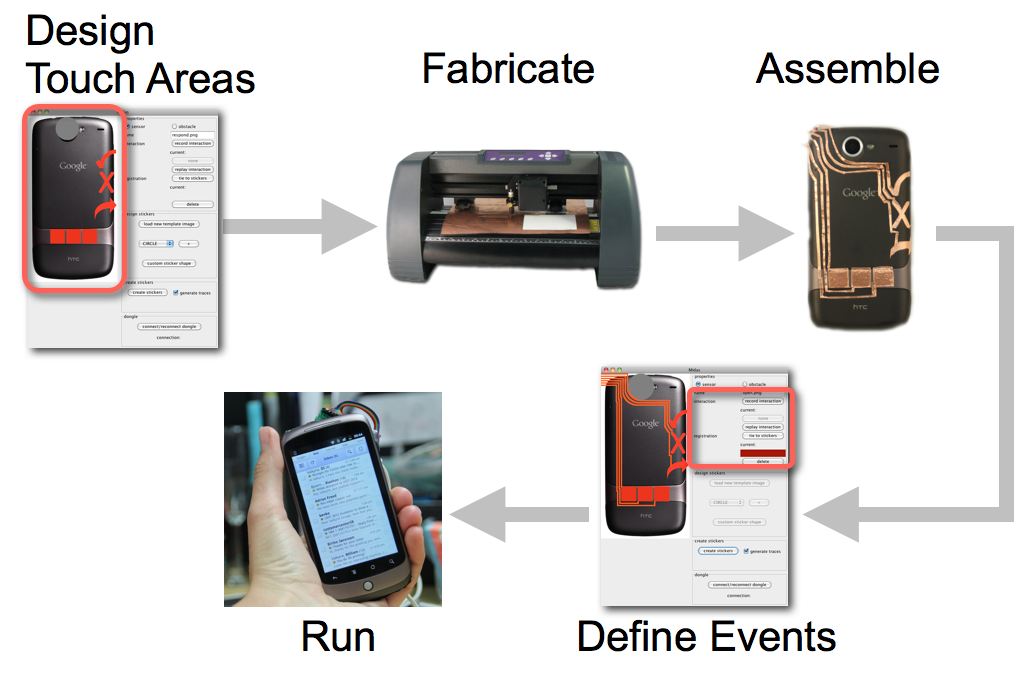
\includegraphics[width=\textwidth]{figures/midas/overview.png}
\caption{Midas enables users to define discrete and continuous touch sensors with custom shapes and layout. It generates fabrication files and assembly instructions. Designers can also define the interaction events of their prototype.}
\label{fig:midas-overview}
\end{figure}

\section{Introduction}

%\valkyrie{How is Midas related to other projects in thesis? How are capacitive interfaces important, how are they seen today}

Ubiquitous, cheap microprocessors have led to a vast increase in consumer products with built-in digital user interfaces. Many of these devices---thermostats, game controllers, and personal medical devices, to name a few---rely on touch sensing to provide input to their user interfaces.

The rise of the iPhone and subsequent touchscreen-based smartphones has been a very visible use of touch input, however these devices rely on software to prototype and create interactions. An app designer can create an interactive graphical user interface using on-screen prototyping tools, purely software with no hardware required. For devices where touch input is not co-located with screen output, for example when a designer wants inputs on the back of a screen (for example to avoid the fat finger problem \cite{baudisch-nanotouch}) or on a device with no screen at all, prototyping becomes much more complicated.

%Digital fabrication processes like 3D printing and CNC machining make it easier to prototype the \emph{form} of such products, enabling designers to go directly from a digital 3D model to a physical object. In addition, user interface prototyping tools have lowered the threshold to connect sensors to graphical user interfaces. However, one main limitation of current toolkits such as Phidgets~\cite{greenberg-phidgets}, d.tools~\cite{hartmann-dtools}, .NET Gadgeteer~\cite{villar-gadgeteer}, or Arduino~\cite{arduino} is their reliance on pre-packaged, off-the-shelf sensors such as momentary switches or slide potentiometers.
Using pre-packaged sensors has important drawbacks. It {\em constrains exploration}: pre-defined physical form factors restrict the space of realizable designs. For example, available buttons can be too bulky or too small, or sliders may be too long or too short. Most sensors also lack {\em physical flexibility}: they are not easily applied to non-planar surfaces or added to existing objects. Finally, a large {\em gulf of execution} remains between digital design files and physical prototypes: sensors must be manually placed and wired one-by-one. This process is tedious and error-prone; physical prototypes can easily deviate from digital design files if a wire is incorrectly placed or forgotten. %While recent research has introduced tools to create touch sensors of different shapes~\cite{holman-tactiletape,hudson-boxes,wimmer-tdr}, their efforts focus on rapidly-constructable, low-fidelity prototypes. In contrast, 
Our work leverages digital design tools and enables designers to use the growing range of fabrication processes to create custom, durable, replicable, iterable, and shareable touch sensors.

We take inspiration from the success of GUI editors. These editors enable designers to specify layout, size, and characteristics of widgets. They also isolate designers from specifying the ``plumbing" that connects widgets to event callbacks. {\em Midas seeks to make the creation of physical touch-sensing interfaces as fluid as the creation of graphical user interfaces in GUI editors.}

Midas is a software and hardware toolkit to support the design, fabrication, and programming of custom capacitive touch sensors (see Figure~\ref{fig:midas-overview}). With Midas, designers first define the desired shape, layout, and type of touch sensitive areas and obstacles in a {\em sensor editor} interface. Designers can choose from buttons, 1D sliders, and 2D pad sensors. For discrete (button) inputs, designers can use polygon shapes or import graphics to define custom shapes; other types are adjustable in size and aspect ratio. Once a designer settles on a layout, Midas automatically synthesizes appropriate capacitive touch sensor pads and routes connecting traces, avoiding user-defined obstacles, to a central touch sensing module via a circuit board grid routing algorithm~\cite{lee-maze}. Midas then generates layout files and step-by-step instructions that designers use to fabricate the sensors using rapid manufacturing techniques. Our prototype cuts sensors from adhesive-backed copper foil and vinyl on a commercial vinyl cutter. We also demonstrate using a circuit board milling machine and a Silhouette Cameo paper cutter to fabricate Midas sensors. Designers then transfer their flexible, adhesive-backed sensors onto the target object and connect the fabricated sensors to a small microcontroller using the routed connections. The microcontroller detects touch events using charge-transfer sensing~\cite{philipp-chargetransfer} and forwards events to a PC. Once assembled, designers can define interactivity on the PC using the sensor editor. Midas supports both record-and-replay actions to control existing local applications, and WebSocket event output for novel and remote applications. WebSockets enable designers to write touch-sensitive applications using standard Web technologies (HTML and JavaScript).

We demonstrate Midas's expressivity with a number of examples. The authors used Midas to create several touch-sensitive interfaces, including recreating prototypes of existing and published systems.

The main contributions this chapter describes are: \begin{enumerate}
\item a novel method to create custom-shaped, flexible capacitive touch sensors by synthesizing sensor pads and auto-routing connections, as well as instructions for assembly and use, from a high-level graphical specification
\item a design tool using this method to enable users to to fabricate, program, and share touch-sensitive prototypes
\item an evaluation demonstrating Midas's ability to create a variety of functional prototypes quickly and cheaply
\end{enumerate}

\subsection{The Geometry-Sensing Link}

For the Midas project, we exploit the convenience of algorithmic routing. The designer creates a sensor layout which matches with her desired aesthetics and objects, then the machine performs the task of creating structures that allow the designer to detect user interactions with the sensors. This is convenient for the designer, as the task of laying out traces is hardly a glorious one, and it may require additional skills and knowledge about reasonable trace widths and the layout of the sensing board. The layout is our link to sensing: the machine knows the routing, thus it has \emph{a priori} knowledge of what it will be sensing. When an interaction triggers a change in capacitance, Midas associates this with the linked sensor and begins the programmed response.

\section{Designing with Midas}
    \subsection{Users}
    
    The target users for Midas are designers who have 2D layout expertise, but who lack experience in electronics and potentially also programming. We target these types of designers through affordances familiar from graphic design programs, instruction-based assembly using a single hardware component, error detection/correction, and easy-to-use sensor output.

Midas echoes graphic and Graphical User Interface (GUI) design programs, offering designers a familiar drag-and-drop interface. Midas also supports scaling via direct manipulation, and has the ability to import custom sensor shapes as PNG images.

The instructions generated by Midas walk designers through machine setup, sensor fabrication, and microcontroller connection. This instruction set assumes no knowledge about the machines, fabrication process, or electronics, and uses color-coded wiring to ensure circuit legibility.

In the case where setup goes awry, Midas can detect two common fault types by performing pattern recognition on its sensor inputs. The faults are ``stuck on'', when sensor traces are too close together and are touching or capacitively coupled, and ``flicker'', when the microcontroller's connection to a sensor rapidly changes and indicates a poor attachment.

Midas's sensor output is available for interaction design via two channels: designers can record literal clicking and typing events on their screen that will be triggered by a sensor input (``record-and-replay''), or they may use JavaScript, a programming language with which many designers are familiar, to accept the events in the form of WebSockets messages for further processing in an interactive webpage.

These usability features will be discussed in more detail in the implementation section.

    \subsection{Design Walkthrough}
    
    We discuss the interface affordances and the
workflow of Midas (Figure \ref{fig:midas-overview}) with a concrete running example:
A designer would like to explore back-of-device and
bezel (off-screen edge) interactions for a mobile phone. In particular, she
would like to scroll through a list of emails with a slider on
the back of the device, and open, reply to, and delete messages
via sensors on the bezel under the phone user's thumb.

        \subsubsection{Drawing Sensors}
Users start by loading an image of the physical prototype
they want to augment into Midas's sensor editor. The sensor
editor (Figure \ref{fig:midas-editor}) allows a user to create the sensor layout, and
define interactive behavior for each sensor. The background
device image helps designers with correct scaling and positioning.
Currently, Midas supports 2D images, including
flattened 3D models. Future work will investigate direct support
of 3D models. Sensor positioning works analogously
to a GUI editor; users choose sensor types and drag them to the desired location on the canvas. Midas supports individual
discrete buttons, one-dimensional sliders, and two-dimensional
pads. Buttons can take on arbitrary shapes---
users can import any graphics file (in PNG format) or draw
custom polygons. Sliders and pads are currently restricted
to rectangular shapes; however, their size and aspect ratio
can be modified to fit the requirements of the prototype at
hand. Users may also define obstacles using the same drawing
tools to restrict routing---Midas will route connections
around these obstacles.
In our phone example, the designer creates one slider and
three discrete buttons. For the buttons, she loads custom
shapes created in a drawing program. She defines a circular
obstacle around the phone's camera so the camera will
not be obscured during connection routing.

\begin{figure}[b!]
\centering
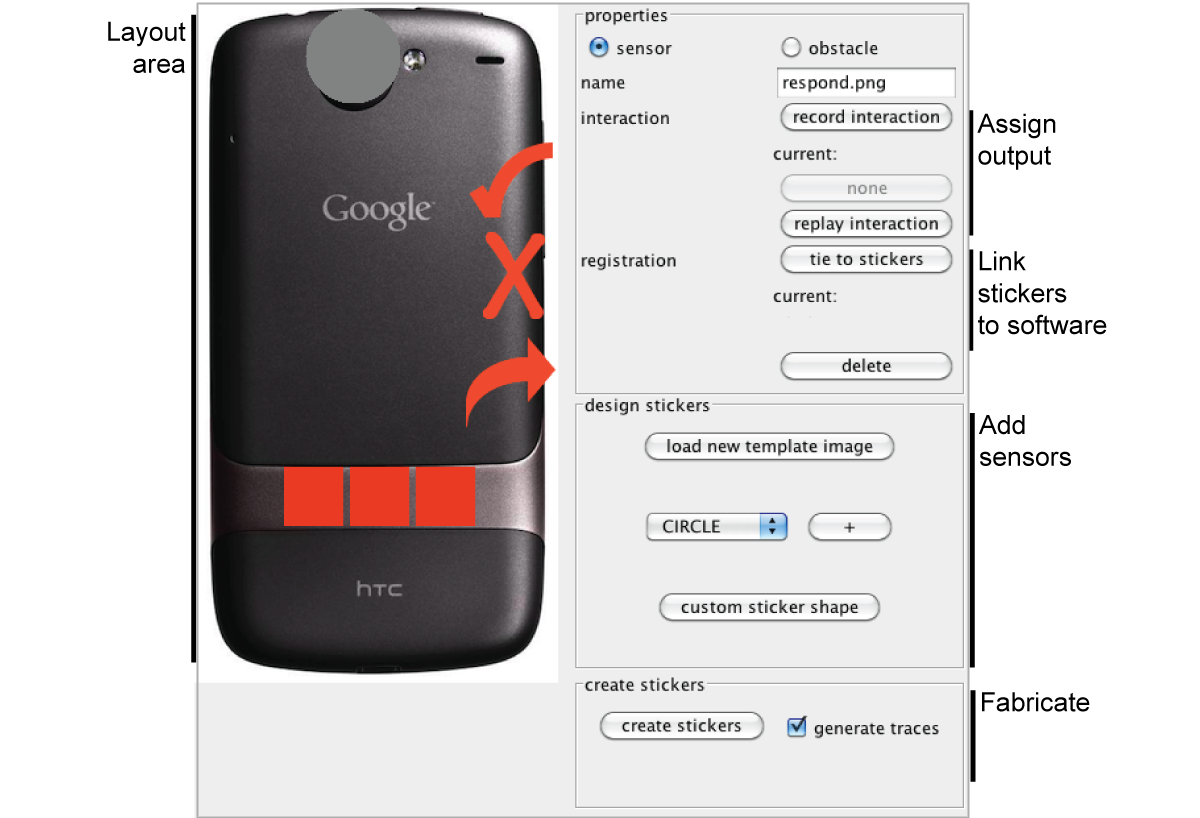
\includegraphics[width=\textwidth]{figures/midas/ui.png}
\caption{Midas's sensor editor takes its cues from GUI editors: designers first lay out sensing areas through direct manipulation; they later define interactions for each sensor using a property inspector.} 
\label{fig:midas-editor}
\end{figure}


        \subsubsection{Fabricating and Applying Flexible Sensors}
Once users complete a layout, clicking the ``Create Stickers''
button generates fabrication files. First, certain components
are automatically split into multiple sensing pads. For instance,
a slider can generate four interdigitated pads (Figure \ref{fig:midas-templates}, third template) for continuous finger tracking, while
2D pads result in two separate layers of triangular pads (Figure
\ref{fig:midas-layering}). Second, Midas generates conductive traces that will
connect each of the pads to Midas's touch controller. An additional mask file, to be fabricated in vinyl, includes cutouts
of only the sensor shapes: it will cover the traces both for aesthetic
reasons and to prevent stray touch events. Midas's connection
routing determines the exact position of each touch
area. Should the user want to experiment with positioning,
Midas can also skip routing and only generate individual
touch pads. However, the user must then manually connect
wires to each sensor and register the sensor in the interface.

The pad creation and routing step generates a set of graphics
files (in SVG format) and an instruction sheet (in HTML)
which appears in the user's browser (see Figure \ref{fig:midas-instructions}). This sheet
contains step-by-step instructions describing how to fabricate
the generated files. For our implementation, instructions include
which SVG files to cut in which material and how to
transfer the cut designs to the prototype object.

In our phone example, the designer generates one SVG file
for the touch areas and one to mask the traces, which prevents
stray touch events. Following the generated instruction
web page, she feeds copper foil into her vinyl cutter and cuts
the corresponding SVG file. She then substitutes a vinyl roll
and cuts a mask layer. As both materials have adhesive backing,
she sticks the copper and vinyl layers onto the phone
she wishes to modify. Once the adhesive layers are applied,
she tapes the end of the routed traces to the Midas hardware,
which is plugged into her computer via USB. Since the design
files for her prototype are digital, she also sends them to
colleagues in another office for a second, remote test. With
the design files and a vinyl cutter, her colleagues can then
recreate a working Midas prototype.

\begin{figure}[t!]
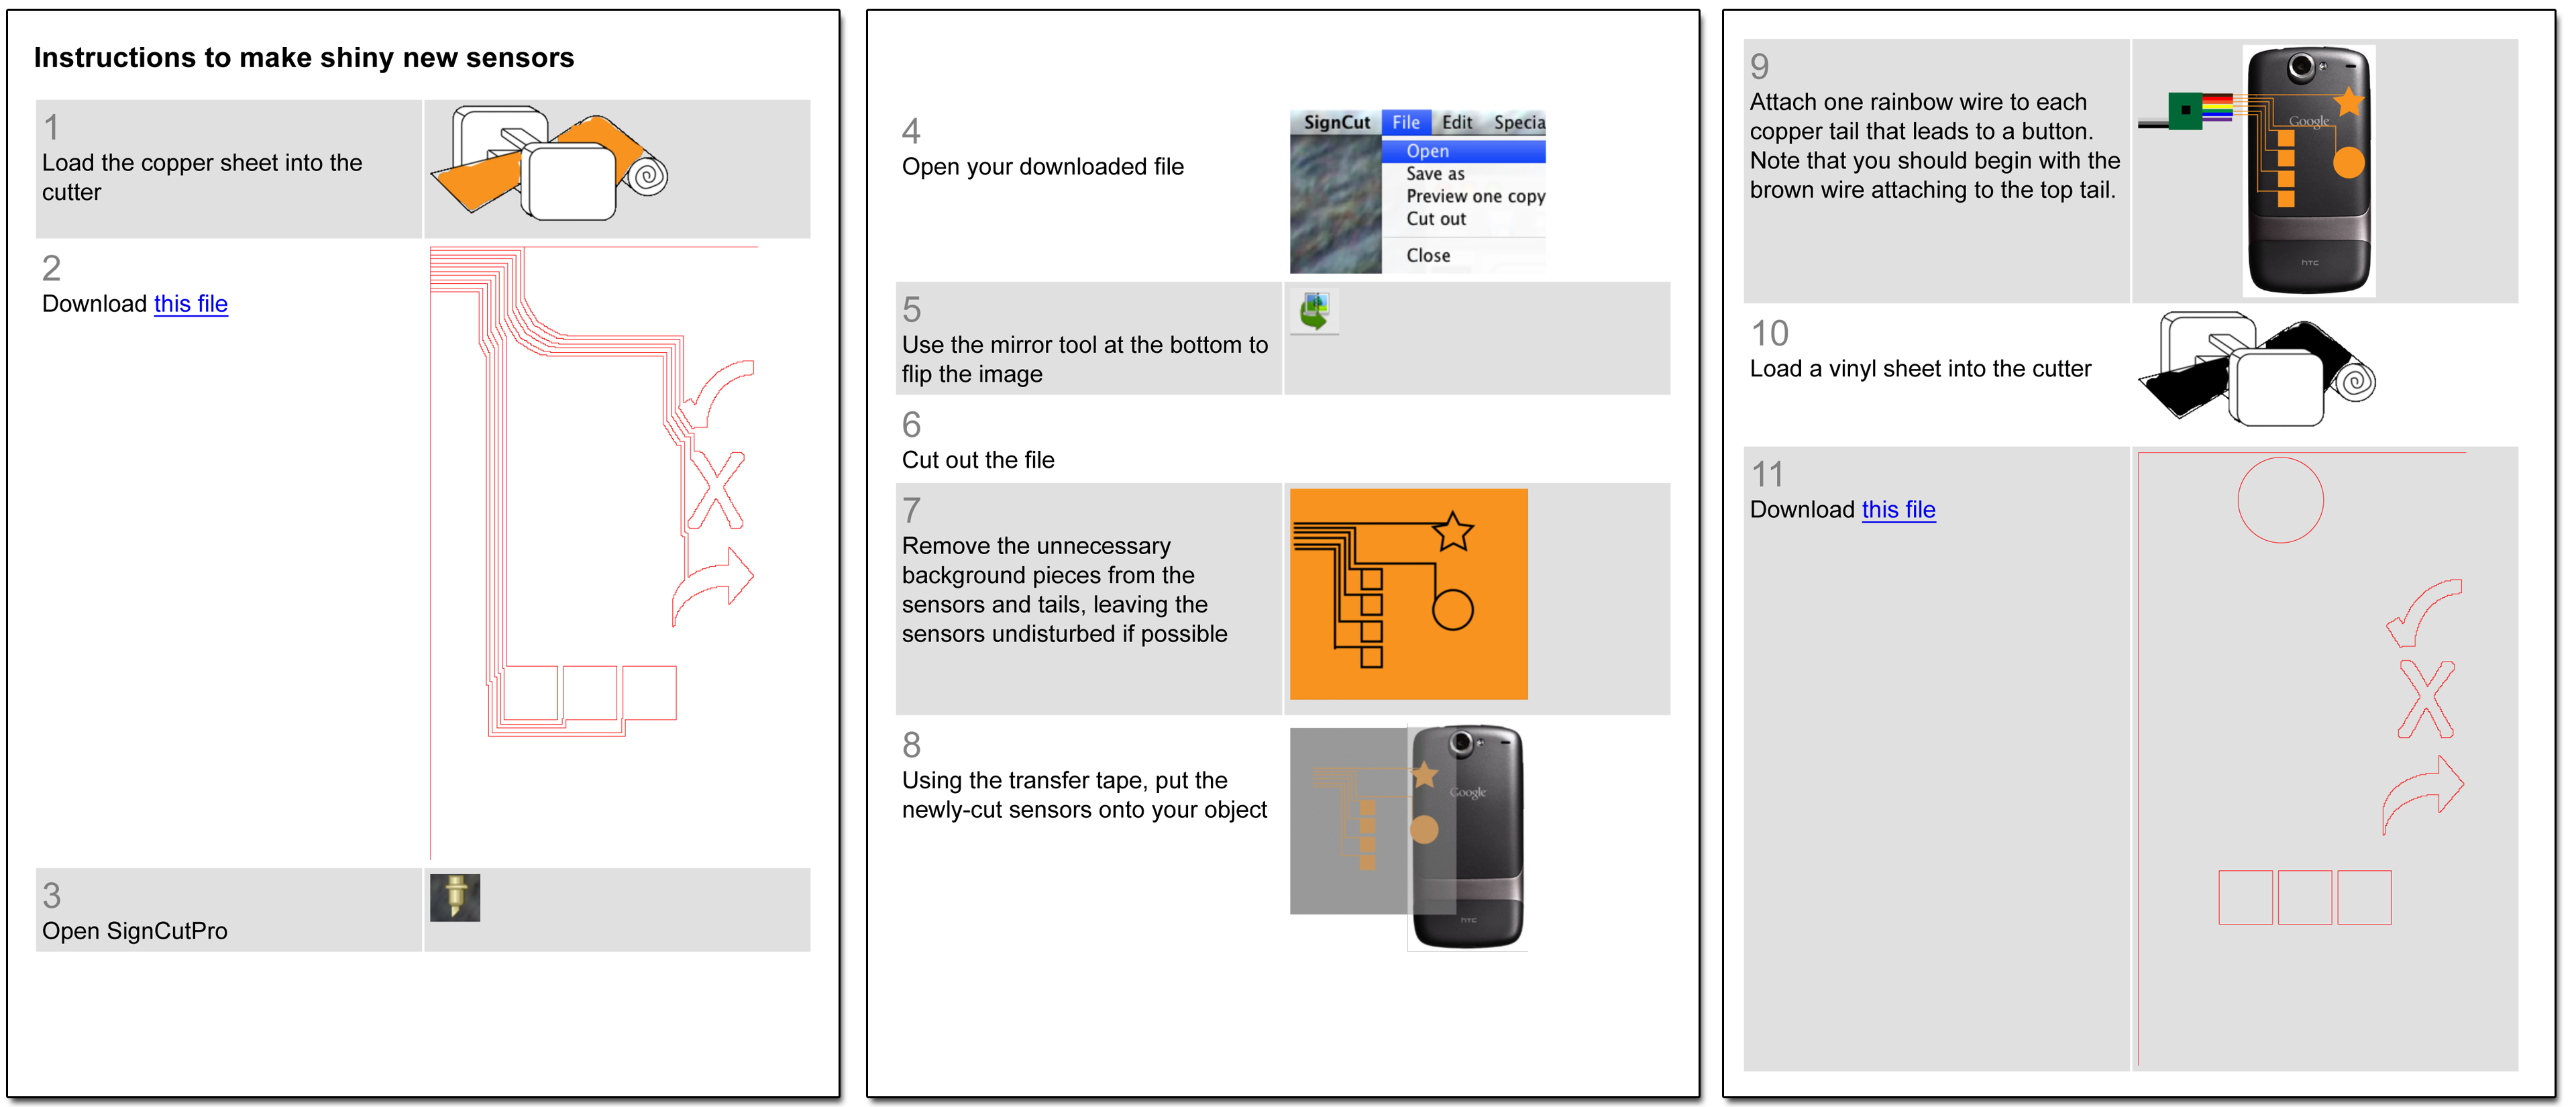
\includegraphics[width=\textwidth]{figures/midas/instructions.png}
\caption{Auto-generated step-by-step instructions in HTML format lead the user through the fabrication and assembly process. Relevant design files are hyperlinked to specific steps; instructions also include general help on processes, e.g., how to use transfer tape to apply a sensor onto an object.} 
\label{fig:midas-instructions}
\end{figure}

        \subsubsection{Connecting Hardware to Software}
Midas senses touch events with a dedicated touch controller
circuit board. Users do not have to program or assemble any
electronics---they may treat the entire setup as a prototyping
“dongle”. Users do have to connect the end of the traces to
the controller's rainbow ribbon cable, either by taping the
cable leads onto copper traces or by soldering them.

To complete a prototype, users return to the sensor editor. In
many toolkits, mapping hardware components to named objects
in software can be error-prone---it is easy to swap wires
or connect to an incorrect pin. If the user prints a fully-routed
design, Midas generates instructions for aligning touch areas
with specific ribbon cable colors. If the user decides to wire 
the design herself, this mapping has to be authored. Midas
uses guided demonstration to assist with this process. For
buttons, the user selects an input element in the UI and clicks
the ``Tie to Stickers'' button; next she touches the corresponding
copper sensor. Midas listens for status change events and
automatically assigns hardware pins. Midas registers sliders
similarly: users are asked to swipe a finger along the slider.

Midas's editor interface displays incoming touch data visually,
re-coloring touched sensors in pink on the sensor editor,
to aid the user in debugging. If something goes wrong during
the connection stage, it is apparent to the user. Midas
also reads the data stream for common errors. If it detects
that two wires may be too close together and triggering each
other, or that there may be a faulty connection from a wire
to the board, that information is displayed to the user in a
connection status area.

\begin{figure}[t!]
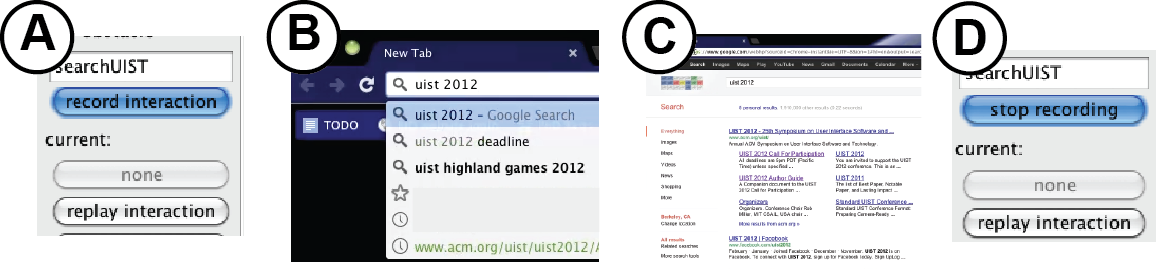
\includegraphics[width=\textwidth]{figures/midas/demonstrate.png}
\caption{Users start to record GUI interactions in the sensor editor (A); they can for example activate the browser, enter text (B), and click on a search result (C), before concluding the recording (D). This sequence of actions can then be triggered by a touch event.} 
\label{fig:midas-demonstrate}
\end{figure}

        \subsubsection{Adding Interactivity}
Designers have two options for authoring interactivity: record-and-replay
of mouse and keyboard events (a strategy adopted
from BOXES \cite{hudson-boxes} and Exemplar \cite{hartmann-exemplar}), or touch event output
to control applications via WebSockets. To record and replay
interactions, designers select a sensor in the editor, then click
on the ``Record Interaction'' button. They can then control any
open application (e.g., start or stop a media player application,
or drag a volume slider). Midas records the generated
keyboard and mouse events and can replay them later in response
to touch input (Figure \ref{fig:midas-demonstrate}).

The types of desktop UI actions that can be executed depend
on the button type. Individual buttons can be tied to an interaction
script, a sequence of keyboard and mouse events
recorded by the user. Sliders are linked to exactly one horizontal
or vertical line on the screen to be controlled by clicks
along its length. 2D pads can control a 2D area on the screen
analogous to a slider area. For sliders and pads, the user must
capture the location on the screen that she wishes to control
with the slider or pad. This is done by clicking at each end
of the slider or in opposite corners of the pad, guided by Midas
prompts. As the user adjusts the sensitivity (number of
discrete buttons) of the slider or pad to be printed, the interaction
with the captured on-screen slider or pad becomes
more fine-grained, also.

Record-and-replay does not require programming, but it is
brittle; changes in application layout or response latency can
break a recorded sequence. To let users author more robust
interactions, Midas uses WebSockets to send touch events
over the Internet. This requires programming, but WebSockets
enable designers to work in the languages many are most
familiar with: HTML and JavaScript.

In our phone example, the designer chooses WebSockets as
she wants to demonstrate how touch events can control a mobile
email application. She creates a mockup in HTML and
writes JavaScript functions to receive touch events.

\section{Implementation}

In this section, we describe the Midas design tool, the hardware it uses for sensing, and fabrication techniques for manufacturing compatible sensors. 

    \subsection{The Midas CAD tool}
    
    We discuss the key parts of the Midas CAD tool: generating sensor pads and routing pads to the touch controller.

        \subsubsection{Generating Sensor Pads}

The Midas sensor editor supports four types of touch sensors:
discrete buttons, two types of 1D sliders, and 2D pads. The
resolution of pads and segmented sliders can be set through a
parameter in the sensor editor. The current editor is written in
Java using the Swing GUI Toolkit. Figure \ref{fig:midas-templates} shows example
templates for each sensor type. The two types of sliders are
based on different sensing approaches. The first, segmented
slider, is made up of individual rectangular touch segments.
Users specify how many segments the slider has. Continuous
sliders offer finer resolution, but require a different detection
approach. We use Bigelow's design of interdigitated electrodes
\cite{bigelow-interdigitated}. In this design, as a finger slides across the pads,
the surface area of the pads underneath the finger changes as
pad digits get smaller or larger. Because capacitance is proportional
to contact surface area, the measured capacitance of
each segment changes during the finger's slide. Though finer
in resolution, only one such slider is supported by our current
sensing hardware. Increasing the number of supported
sliders is possible with additional engineering effort.


\begin{figure}
\centering
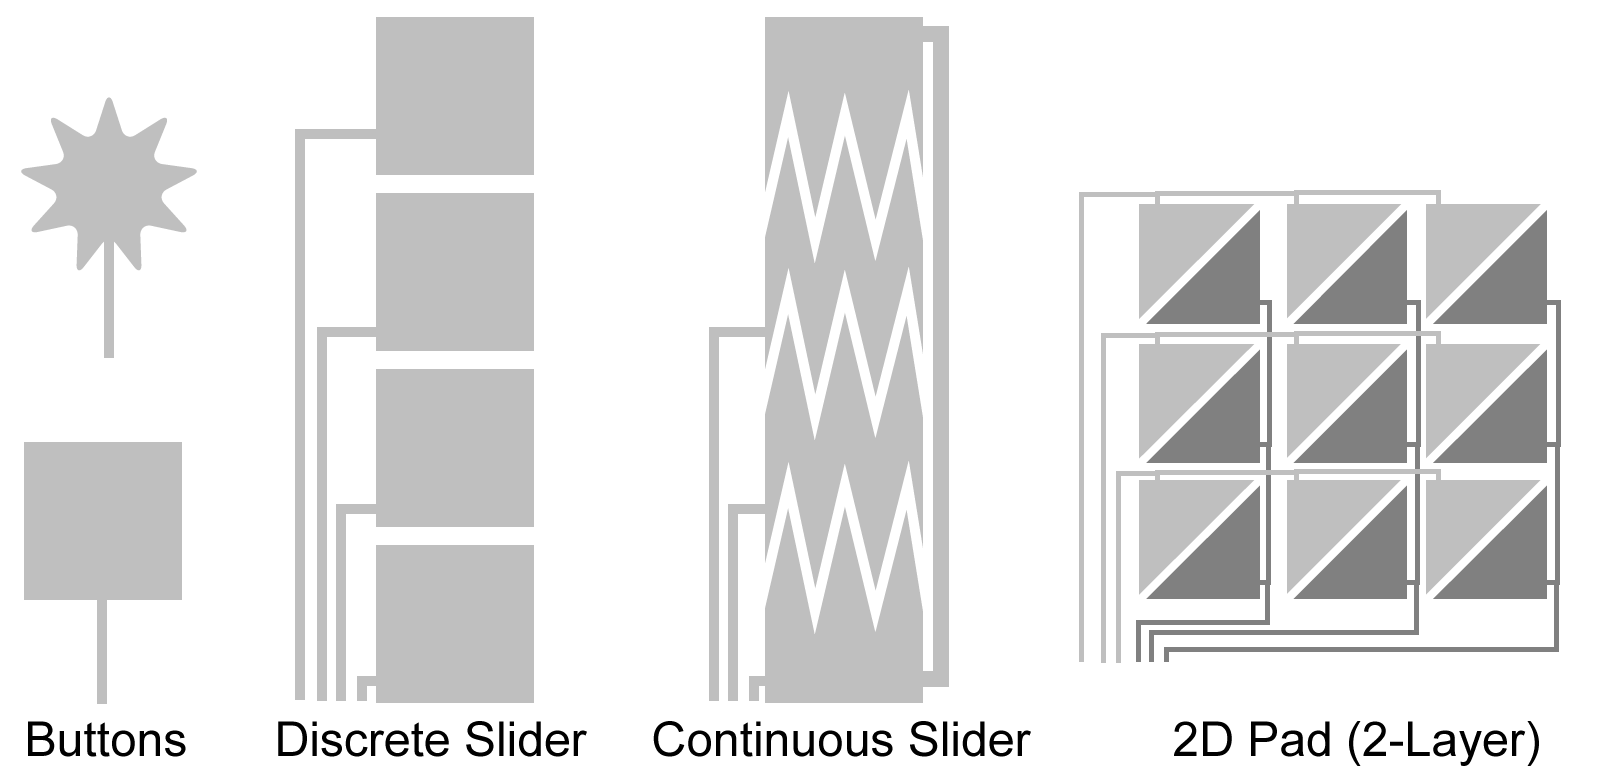
\includegraphics[width=\textwidth]{figures/midas/pad-templates.png}
\caption{Midas can generate four different types of sensors: discrete buttons, discrete sliders, continuous sliders, and 2D pads. The pad uses row-column scanning and requires multi-layer construction because traces cross.} 
\label{fig:midas-templates}
\end{figure}

\begin{figure}
\centering
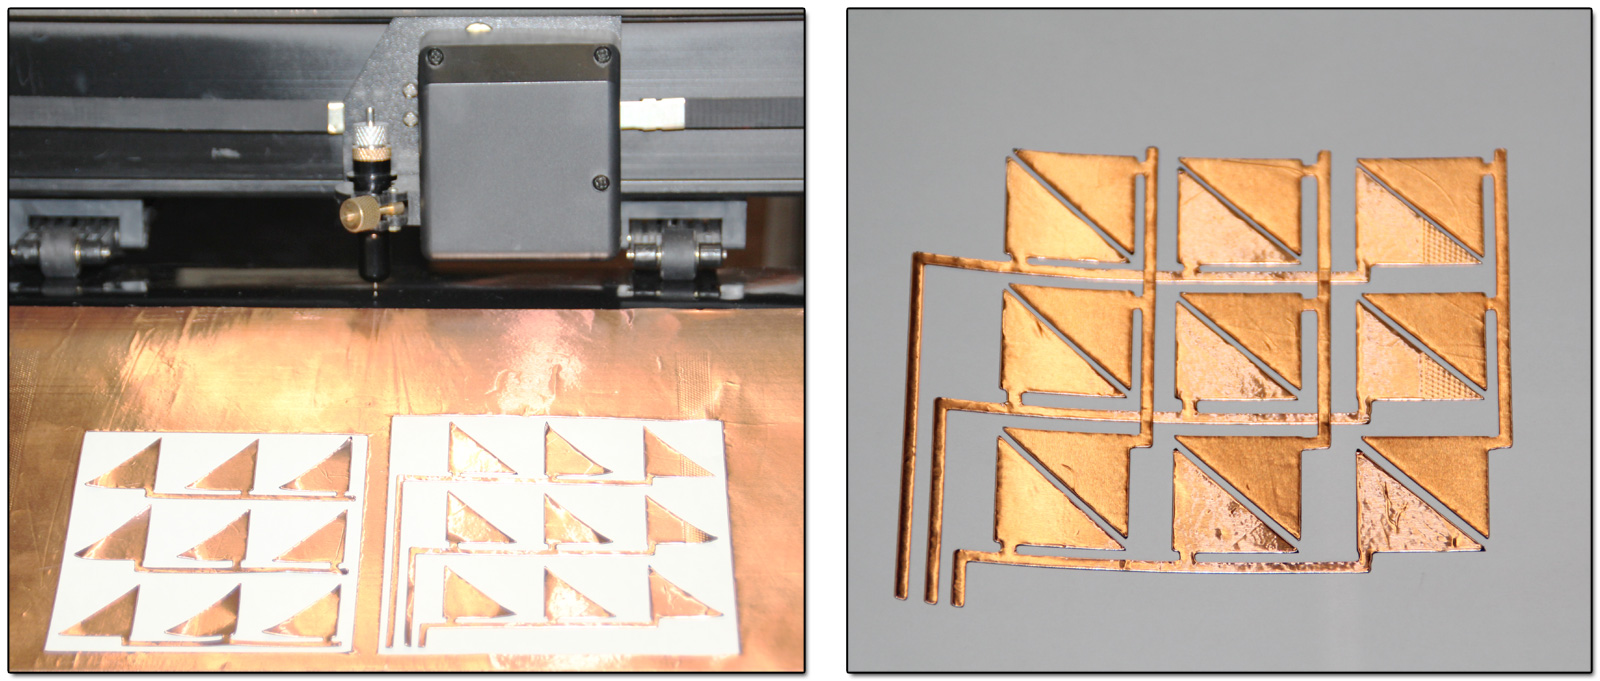
\includegraphics[width=\textwidth]{figures/midas/2dgrid.jpg}
\caption{2D pad sensors are fabricated in two different layers that are then superimposed. Because each copper layer has a vinyl backing, no other inter-layer masking is required.} 
\label{fig:midas-layering}
\end{figure}

2D pads use row-column scanning to reduce connecting traces.
For example, a $5 × 5$ array requires $25$ individual traces, but
only $5 + 5 = 10$ row-column traces. This design requires a
dual-layer construction where horizontal traces are isolated
from vertical traces. We use copper foil applied to vinyl foil
in our cutter, so each layer already has an insulating substrate.
Designers thus first apply the bottom conductive layer,
then place the top layer directly over it (see Figure \ref{fig:midas-layering}).
To create a mask layer that covers the topmost copper traces,
we generate a design file containing pads from all layers, but
no traces. This layer is cut in vinyl. While for other layers
designers transfer the pads and traces, for the mask layer they
peel and transfer the surrounding “background” shape with
sensors and obstacles cut out (see Figure \ref{fig:midas-poster}, left).


        \subsubsection{Routing Pads to the Touch Controller}
Midas employs an auto-routing algorithm to generate conductive
traces connecting electrodes to the Midas touch controller.
User-defined obstacles are avoided. We implement
Lee's breadth-first maze routing algorithm for single layer
paths \cite{lee-maze} (see Figure \ref{fig:midas-routing}). This algorithm selects a source and target (the source is the trace anchor for connecting to the microcontroller, the target is all pixels on the perimeter of the sensor). Then, beginning at the source, floods the grid by marking each viable pixel---i.e., pixels which are not on obstacles and which will not touch other sensors---with its distance from the source. When any of the target locations are reached, the algorithm traces back through the marked pixels, maintaining straight traces as much as possible, and generating a trace along the path selected. For 2D pads, we perform two independent routings:
one for the row layer and one for the column layer. Our
current algorithm does not generate vias (connections between
different conductive layers). When auto-routing fails,
we employ an iterative search by adjusting the position where
traces connect to sensor pads, routing the sensors in a different
order, or moving the position where target traces connect
to the touch controller. In our experience, this basic routing
algorithm has performed adequately, though there are designs
that cannot be successfully routed. For such cases, the
algorithm could be replaced with more sophisticated routing
techniques that include user input, though such techniques
require that the user has a correct mental model of the routing
process.

Midas currently offers generic suggestions when routing fails,
e.g.: “Sensor reply may be too close to sensor delete. Try
moving sensors away from the edge and each other.”

\begin{figure}[t]
\centering
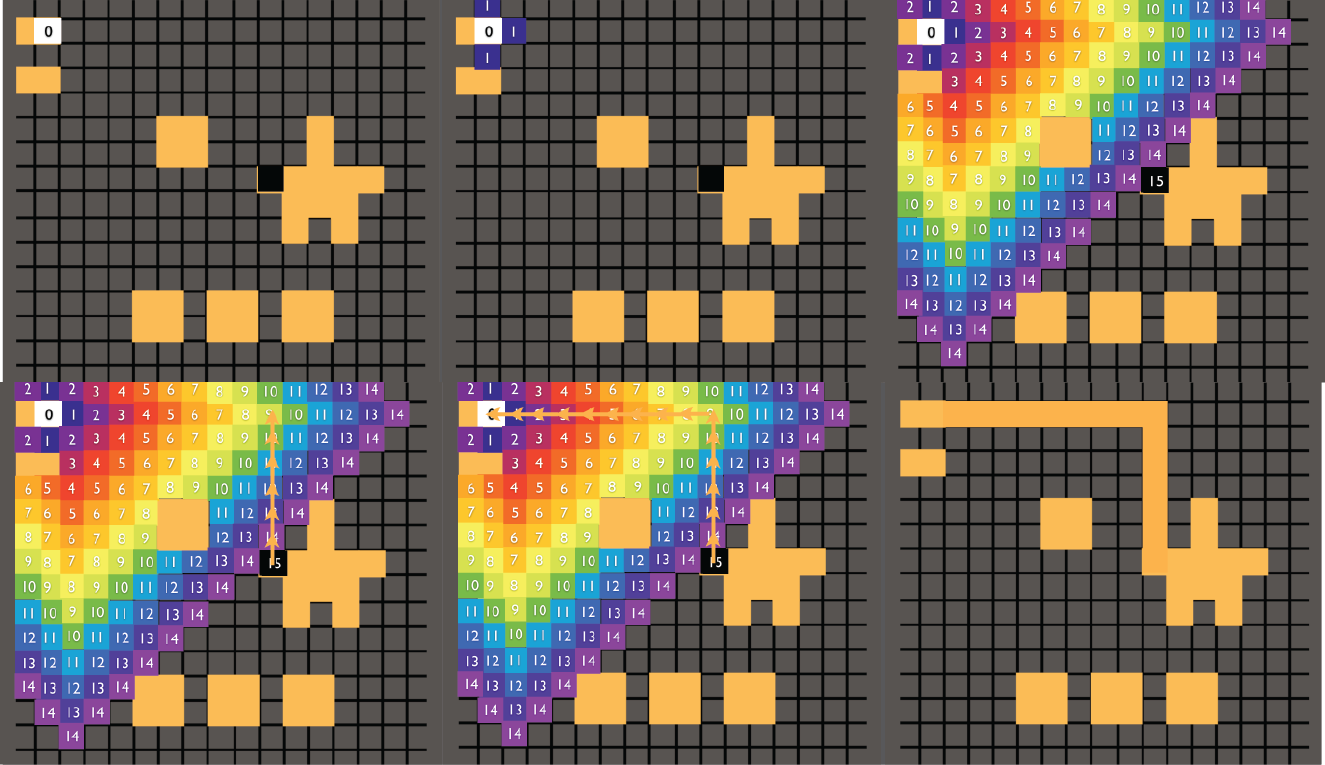
\includegraphics[width=\textwidth]{figures/midas/routing.png}
\caption{The Midas routing algorithm, based on Lee's \cite{lee-maze}, first selects a source and target point. It then floods the grid, beginning at the source, marking each viable ``pixel'' as one further than its pre-marked neighbor. Once the target has been reached, the algorithm traces back through the marked pixels (we selected to make vertical moves before horizontal) to the source and creates a trace.} 
\label{fig:midas-routing}
\end{figure}


    \subsection{The Midas Hardware}

We discuss the components of the Midas hardware: the mechanism of capacitive touch sensing and the fabrication of compatible sensor pads. We also describe how the sensed and digitized signal is used to design interactions.

    \subsubsection{Sensing Mechanism}

        Midas relies on capacitive touch sensing. The original Midas touch controller (Figure~\ref{fig:midas-microcontroller}) is based on an Atmel microcontroller board~\cite{teensy} and capacitive sensing chips from Quantum (QT1106) and Freescale (MPR121) Semiconductors. For discrete inputs, both chips rely on charge-transfer sensing using single-wire electrodes: the electrodes are part of a simple RC circuit in which an output pin is set high, and time is measured until an input pin also reads high. This time is proportional to the capacitance of the circuit: when a person touches an electrode, the circuit capacitance and the charge transfer time both increase. The Quantum chip also implements Bigelow's design to extract continuous position readings from interdigitated electrodes by interpolating based on relative capacitance between neighboring pads~\cite{bigelow-interdigitated}. The microcontroller runs software written in embedded C to interface with the sensor chips and communicates touch data to a connected computer over USB. It recalibrates the touch sensing chips periodically to ensure floating sensor values do not lead to erroneous touch readings.
        
        Our new Midas touch controller uses an Adafruit Blufruit microcontroller with Bluetooth compatibility. It does not implement Bigelow's interdigitated sensing but could do so in the future; for discrete sensing it leverages the Arduino CapSense library\footnote{\url{playground.arduino.cc/Main/CapacitiveSensor?from=Main.CapSense}} which uses two-wire electrodes; it determines the capacitance by timing the charge transfer time between the pins. The new board design also has sturdy milled connection pads to attach to traces; these can be attached using Z-axis conductive tape (e.g., 3M's Z-Axis Conductive Tape 9703). This board transmits sensed readings directly to a phone over a Bluetooth connection.
        
        \begin{figure}[b]
        \centering
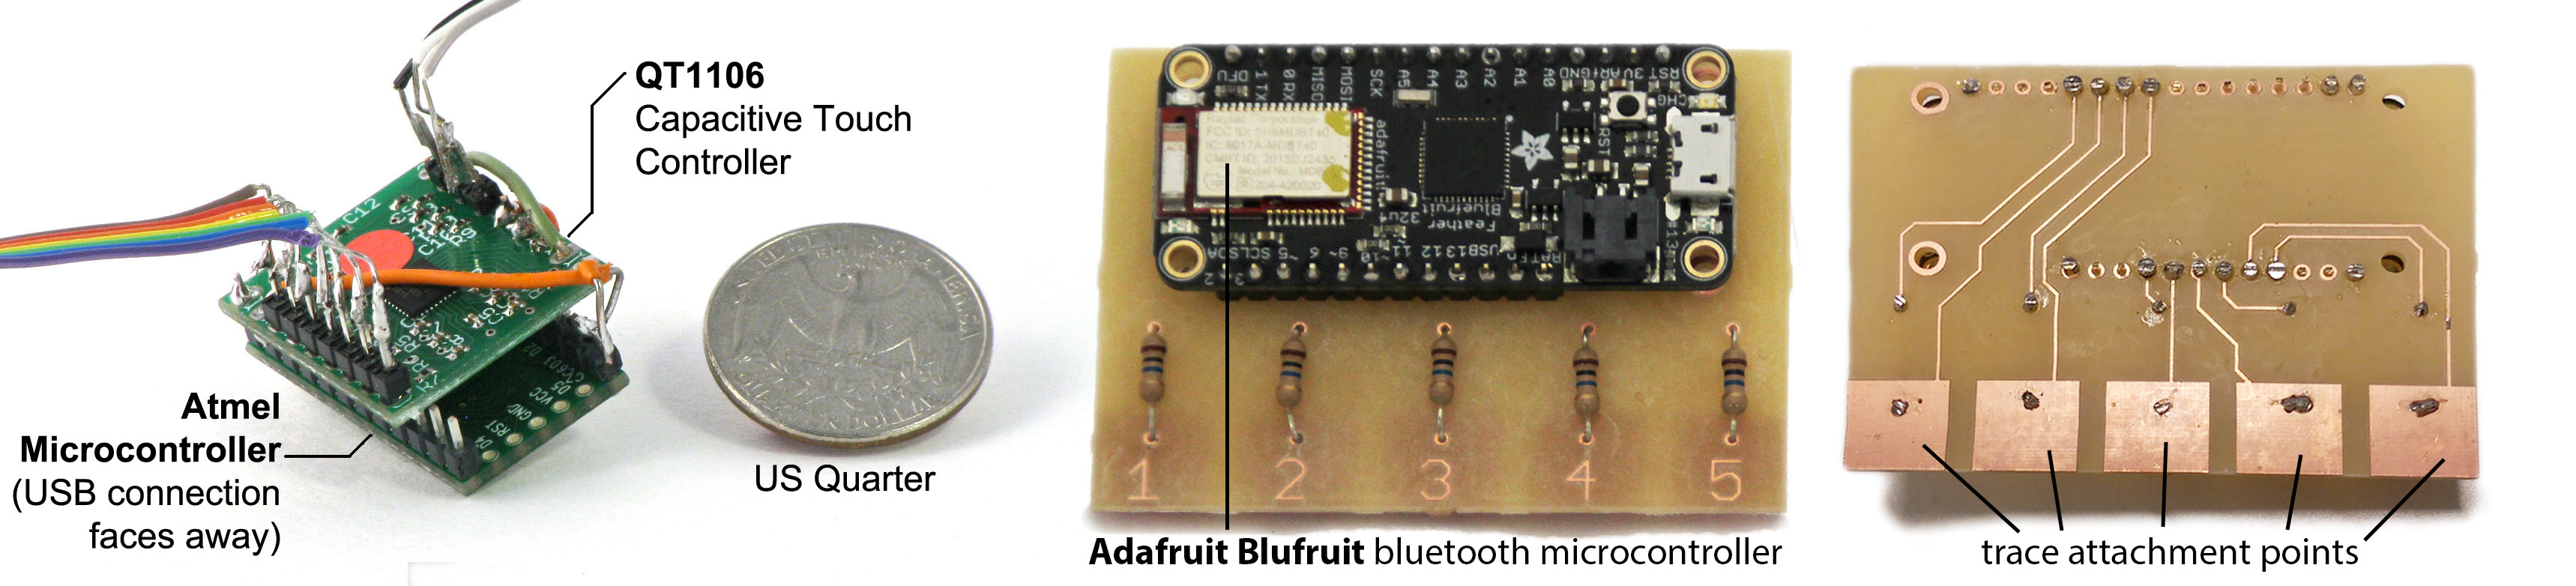
\includegraphics[width=\textwidth]{figures/midas/microcontrollerz.jpg}
\caption{The original Midas touch controller board (left) uses a commercial capacitive charge transfer detection chip to sense touch events. Events are relayed to a computer via a mini USB connection on the back. The ribbon cables are used to connect to the end of routed traces. The new board (right) uses an Arduino touch sensing library and a Bluetooth-compatible microcontroller for wireless data transmission and sensing. A US quarter is shown as a size reference.} 
\label{fig:midas-microcontroller}
\end{figure}

    \subsubsection{Fabrication}
    
    \begin{figure}[b]
    \centering
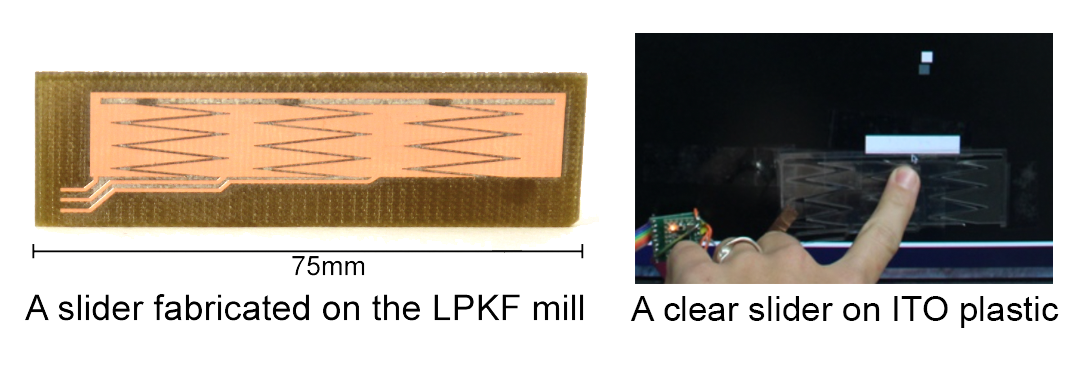
\includegraphics[width=\textwidth]{figures/midas/otheroptions.png}
\caption{Two example touch sensors fabricated with alternative processes: left, a hard sensor created on a circuit board mill. Right, a sensor cut from Indium Tin Oxide-coated transparent plastic..} 
\label{fig:midas-dimatix}
\end{figure}

Midas generates vector graphics files in SVG format for the
electrode and mask layers. These files can be used to control
digital fabrication processes. Our prototype currently
cuts conductive, adhesive-backed copper foil on a commercial
vinyl cutter---a plotter with a cutting knife instead of a
pen. This medium has multiple advantages. First, it is cost-effective
and readily available: vinyl cutters are in the same
price range as laser printers (ours, a tabletop model with a
$35cm$ bed, cost \$$200$); and copper foil costs a few dollars
per foot. Second, copper has excellent conductivity. Third
flexible, adhesive foil is easy to apply to non-planar surfaces.
However, there are important drawbacks as well. Most importantly,
the cutting process and manual weeding (removing
background material) determines a minimum feature size
for traces. Thin geometric features can also break during
transfer, and the weeding process can be tedious and time-consuming.
We found the most success adhering
the copper sheets to vinyl sheets and cutting both layers at
once. This setup has the added benefit of allowing designers
to prototype touch interactions on conductive surfaces (e.g.,
aluminum casing) as vinyl is an excellent insulator.
Alternative fabrication processes may be preferable to copper
foil cutting when higher precision or durability is required.
Three promising approaches are circuit board milling, which
can produce smaller features but is limited to rigid boards; cutting from Indium Tin Oxide (ITO)-coated plastic, which allows for transparent sensors but is not self-adhesive and is less flexible than vinyl;
and conductive inkjet printing, which can produce the smallest
features, but is not yet available to many end users. As
a proof of concept, we produced a touch sensor on an LPKF
circuit board milling machine, and one on a Silhouette Cameo paper cutter (see Figure \ref{fig:midas-dimatix}).

\subsubsection{Debugging}

Midas offers basic debugging support. The interface displays incoming touch information from the microcontroller, highlighting activated sensors. We have also implemented basic regular expression filtering on the touch stream to help the user identify potential problems. A time-stamp and code representing each touch event is stored in a stream. When a sensor is ``stuck on'' for more than $10$ seconds, Midas reports that that sensor may be touching another wire. When a touch sensor ``flickers'' on and off more than twice within $500ms$, Midas suggests that there may be a faulty connection from that sensor to the microcontroller.

\subsection{Event Output}
Once the user has assigned interface scripts to sensors, Midas listens for events from the touch controller. When a touch event matches the key of a saved interaction, that interaction's associated script is executed.

\subsubsection{Record-And-Replay}

In record-and-replay, the user selects a sensor and records a sequence of mouse and keyboard actions that should be played back when the sensor is touched. Early prototypes of Midas used Sikuli for this purpose---a scripting language based on computer vision analysis of screenshots~\cite{yeh-sikuli}. While more robust than hardcoded click locations, Sikuli was designed for automation scripts rather than interactive control, and the latency of invoking and executing scripts was too high. Our current prototype uses the Java Robot API~\cite{robots} to captures and replay both mouse clicks and keyboard events. We share this approach with the BOXES system~\cite{hudson-boxes}.

\begin{figure}[b]
\centering
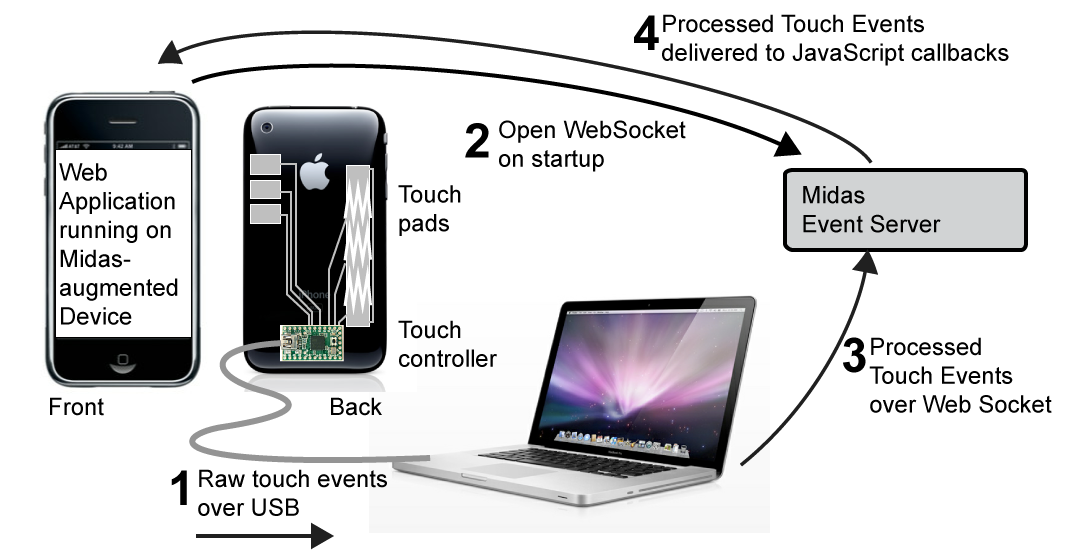
\includegraphics[width=\textwidth]{figures/midas/socket-events.png}
\caption{Midas's socket event output enables designers with programming knowledge to create web applications in HTML and JavaScript that react to touch input outside the screen area of a phone or tablet.} 
\label{fig:midas-socket}
\end{figure}

\subsubsection{WebSocket Communication with Web Applications}

Record-and-replay is restricted to applications running on the same machine as the sensor editor, and it is limited to mouse and keyboard event injection. To surmount this limitation, Midas can also export touch events to remote clients via a built-in server using the WebSockets API. For example, an application running on a smart phone can open a WebSocket connection to Midas and receive a callback for any Midas button, slider or pad event. The callback function receives an event object describing which sensor changed state, and the value of the new state (e.g., on/off, or slider value).

Our WebSockets server is implemented in node.js using the socket.io library. We chose WebSockets because it offers full-duplex communication at low latencies, and, more importantly, is supported by modern web browsers. This means designers can author user interfaces that respond to Midas touch input in HTML and JavaScript. There are two main benefits to these technologies: (1) many designers are already familiar with them from web design; (2) developed interfaces can be deployed on any device with a compatible browser, even if that device does not offer a way to directly connect external hardware. For example, it is difficult to directly connect sensors to Apple's iPhone or iPad.

With our WebSockets architecture (Figure~\ref{fig:midas-socket}), designers open a browser and enter the URL of an HTML file they have placed in the Midas server directory. This file opens a socket connection from the phone browser to Midas. When Midas receives events from the touch controller, it forwards them to the client, which can then show visual feedback.

\subsection{Bluetooth}

Our new touch controller leverages Bluetooth for communication. The detected data are streamed similarly to those in the WebSockets condition, however in this case they are transmitted via Bluetooth, and the receiving device must be paired to the controller.

\section{Evaluation}

    In order to demonstrate that Midas's sensing and fabrication technique fits our criteria of being a cheap, fast, and flexible method of prototyping, we elaborate on each of these criteria below.

    \subsection{Cost-Effective}
    
    Midas enables touch-sensitive prototyping for roughly the cost of a laser printer. The vinyl cutter used for the Midas project, a tabletop model with a $35cm$ bed, cost \$$200$. Copper foil costs a few dollars per foot.
    
    Alternatives to this fabrication method include cutting Indium Tin Oxide (ITO)-coated plastics, using silver ink in an inkjet printer, and fabrication using a circuitboard mill. ITO-coated plastics allow for transparent sensors; ITO costs roughly \$$.25/in^2$ and can be fabricated on an inexpensive paper cutter. Silver ink can be used in many existing inkjet printers, and costs roughly \$$1/mL$ or \$$2/ft^2$ of total coverage. Circuitboard milling has a high startup cost (a suitable machine can cost as little as \$$800$, and upwards beyond that), but the per-unit expense is low, about \$$17/ft^2$.
    
    On the sensor side, the full sensor setup we prototyped with cost \$$36$: \$$16$ for the Arduino Teensy microcontroller board, and \$$10$ for each of the capacitive sensing breakout boards. This cost could be reduced further with custom circuitboards (our setup was assembled from commercially-available boards for expediency), and the setup is can be easily detached from a prototype and reused in a new iteration or for a different project.
    
    \subsection{Fast}
    
    We did an informal first-use study, and it took all participants $<1$ hour to both receive training and create working media player peripherals with the system.
    
    We recruited three participants for this study. Two were graduate students at UC Berkeley (in Computer Science and Mechanical Engineering), and the third was a software engineer at a local technology company. All had some prior experience with prototyping and electronics.

        \subsubsection{Procedure}
Participants received a walkthrough of Midas including a simple record-and-replay task to launch a browser based on a single button input. Participants were then asked to design a physical control interface for a media player (iTunes). No other constraints were given as we wished to encourage exploration. Participants completed a post-task questionnaire with open-ended questions on interface usability and workflow utility.

    \subsubsection{Results}
All participants successfully designed media players (Figure~\ref{fig:midas-study1}). Participants commented positively on how Midas aided them with the task of physical construction---both by routing connections and through the generated instructions. Record-and-replay was easy to comprehend and effective for the given task. Though the task did not require programming, two participants expressed interest in receiving touch events in their own applications. We take this as corroboration for the utility of our WebSocket server. Participants additionally identified several areas for improvement (including more detailed instructions, additional help for auto-routing failures, and additional feedback for touch events), which are included in our most recent design revision, described above.

\begin{figure}[t]
\centering
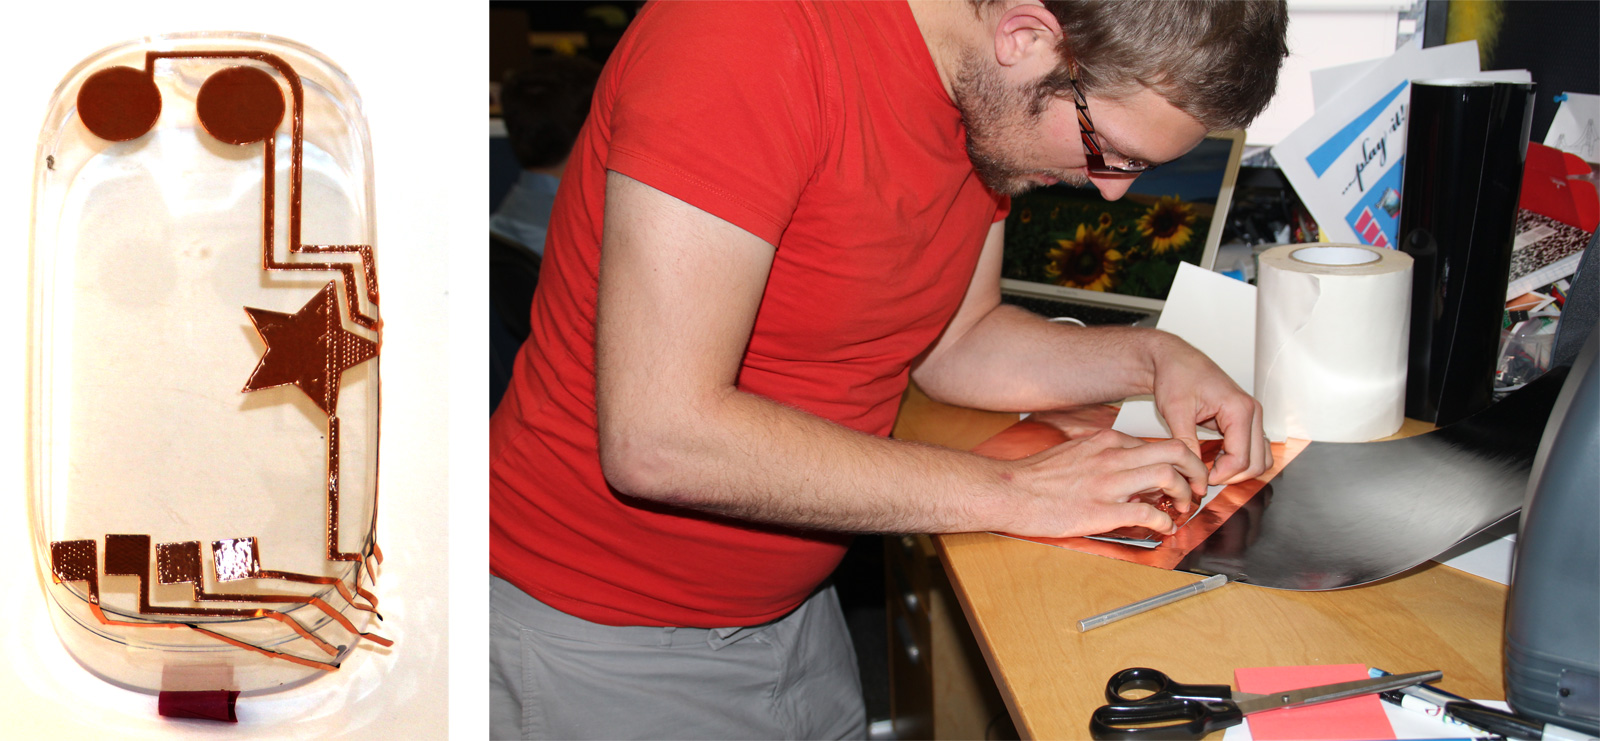
\includegraphics[width=\textwidth]{figures/midas/study1.jpg}
\caption{A study participant's sensor layout for a PC media player peripheral.} 
\label{fig:midas-study1}
\end{figure}

    \subsection{Flexible}
    
    To demonstrate Midas's expressivity, we built several interactive systems that used all sensor types, and output using both WebSockets and record-and-replay.
    
        \subsubsection{Text Entry}
Wobrrock's EdgeWrite~\cite{wobbrock-edgewrite} is a unistroke text entry technique based on activating a series of corner points of a rectangle. Wobbrock demonstrated that this technique can be implemented using four discrete capacitive touch sensors~\cite{edgewrite-cap}. We cut four discrete buttons and a mask with Midas, attached them to the back of a smartphone, and implemented the EdgeWrite recognition algorithm in JavaScript (Figure~\ref{fig:midas-edgewrite}). Using socket events, we demonstrated how EdgeWrite can be used to enter text on the back of a mobile device, leaving the screen unobstructed. The implementation is functional, though latency for detecting single button presses was higher than expected (\textgreater 100ms). We plan to investigate ways to increase responsiveness in future work.

\begin{figure}[t]
\centering
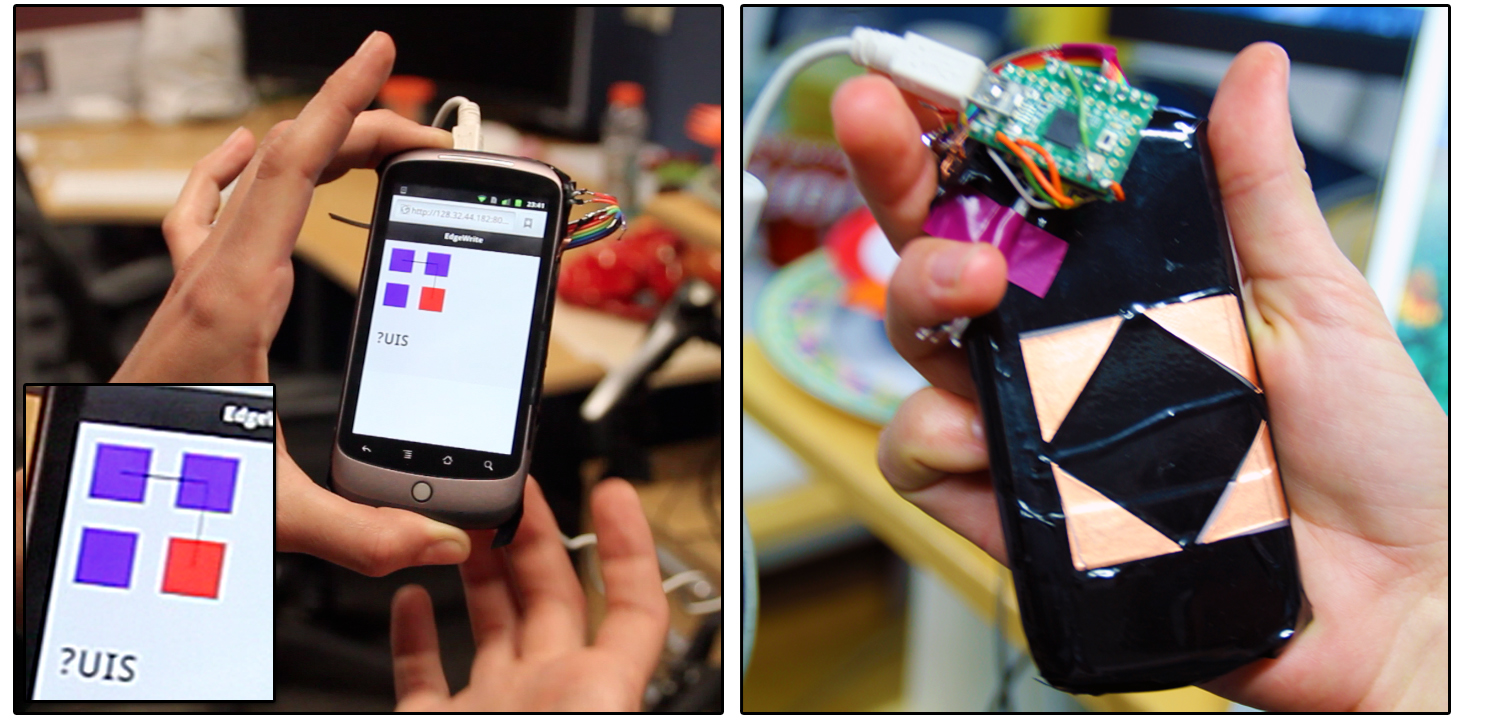
\includegraphics[width=\textwidth]{figures/midas/edgewrite.jpg}
\caption{We implemented Wobbrock's Edgewrite on the back of a cell phone using a 2x2 pad and WebSocket events sent to a web page.} 
\label{fig:midas-edgewrite}
\end{figure}

        \subsubsection{Game Controller}
To test the responsiveness of Midas's continuous slider, we created a simple game controller for Breakout, in which players horizontally position a paddle to bounce a ball into layers of blocks (see Figure \ref{fig:midas-dimatix}). In less than fifteen minutes, we attached the slider and mapped slider position to paddle position using record-and-replay.
The slider is more responsive than individual buttons, and we were able to control the paddle accurately enough for gameplay. The slider's response is non-linear across certain regions, however. Accounting for this is left to future work; our instinct says that it may be caused by electromagnetic interference from the thin traces and sharp right angles in the design.

We fabricated two versions of this game controller: one from a circuitboard milled slider, and a second from Indium Tin Oxide (ITO)-coated transparent plastic. This underscores the point that only the conductivity of the material is important; whether it is flexible/rigid or opaque/transparent has no bearing on the functionality.

        \subsubsection{Music Postcard}
At a recent media festival, a promotional poster printed with conductive ink enabled passersby to select and play music from a number of artists by touching corresponding areas on the poster~\cite{paperposter}. We implemented a postcard-sized version of this poster (Figure ~\ref{fig:midas-poster}). We scaled back the size to conserve resources; large designs are possible and only restricted by the cutter's bed width. Our version uses six discrete buttons and one continuous slider to control playback and volume of music clips on a desktop computer. We again cut a vinyl mask layer to prevent stray touch events. We used Midas's record-and-replay function to remote control the iTunes music player.

\begin{figure}[t]
\centering
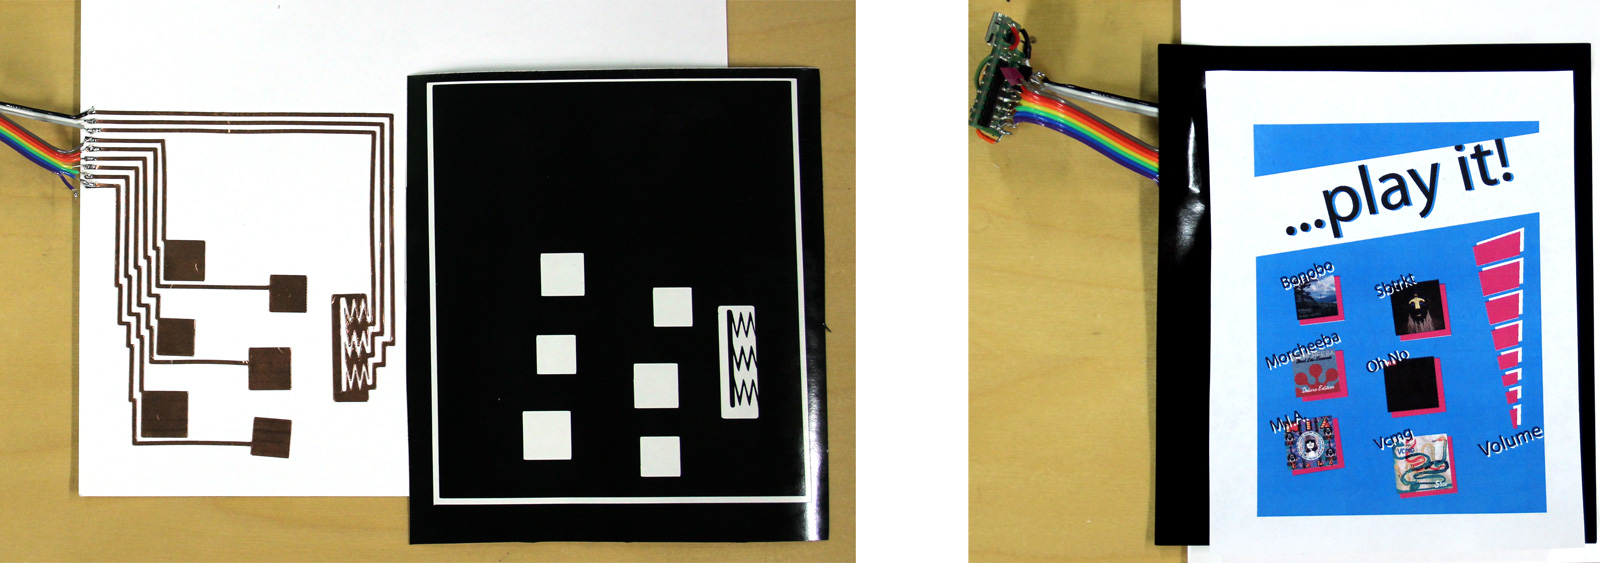
\includegraphics[width=\textwidth]{figures/midas/poster3.jpg}
\caption{Our music postcard lets users sample tracks by different artists. Left: Circuit and mask layer; Right: assembled postcard.} 
\label{fig:midas-poster}
\end{figure}

        \subsubsection{Papercraft Pinball Machine}
Papercraft is the art of cutting and folding paper into 3D models. To demonstrate how Midas can be used for attaching sensors to more complex 3D shapes, 
%, and there are many popular templates for this hobby. Using this art, 
we created a papercraft pinball machine which can control a pinball game on a laptop. First we downloaded a template design for a pinball machine \cite{indianajones}, cut it out, and assembled it. We then loaded the already-flattened template model into Midas's 2D editor interface and defined the negative space around the model as a routing obstacle (Figure ~\ref{fig:midas-pinball}). This guaranteed that all trace routing would be on the surface of the model. After attaching the two buttons for the bumpers and a continuous slider for ball release control, we used record and replay to control a desktop pinball game.

\begin{figure}
\centering
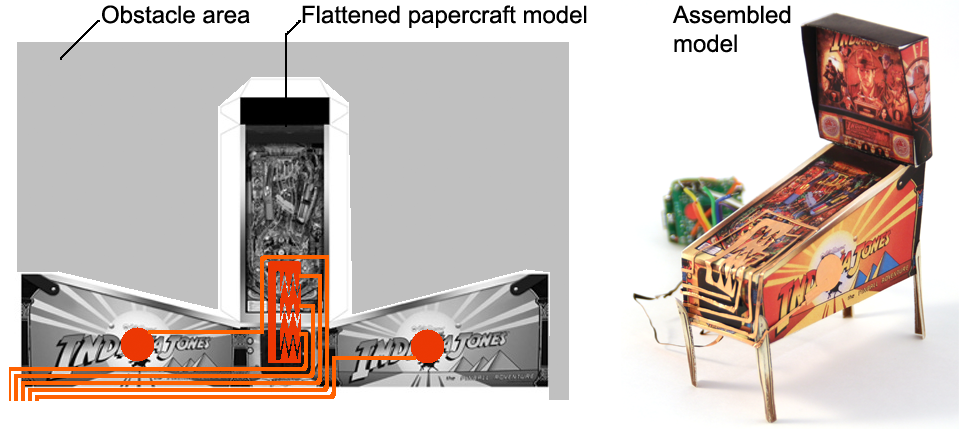
\includegraphics[width=\textwidth]{figures/midas/pinball-horizontal.png}
\caption{For our papercraft pinball machine, we defined the negative space in the template as an obstacle to restrict sensor routing.} 
\label{fig:midas-pinball}
\end{figure}


\section{Discussion}

    Midas, as one of the first fabrication papers in the HCI community, explored a variety of interesting challenges and opportunities around digital fabrication. It serves several purposes well, but there are limitations caused both by the fundamental approach and the particular engineering of our prototype.

    \subsection{Sweet Spots}
    
    Midas is well-suited to prototyping particular kinds of objects. It allows facile testing and iteration on unusual types of touch interactions, for example on the backside of devices: touch screens allow input and output, but adhering a smartphone-like screen to every location a designer wants to sense a touch input is prohibitive. Additionally, unique sensor shapes, like stars or check marks, can be tested with Midas much more simply than with custom-fabricated touchscreens.
    
    Midas opens opportunities for custom sensors on the surfaces of flat or singly-curved objects, as well as 3D objects that are developable \cite{dutton-developable}. While pre-fabricated sensors, such as those used for prototyping with Arduino \cite{arduino} or d.tools \cite{hartmann-dtools}, can enable prototyping on flat surfaces, they are typically not flexible and thus cannot be applied to non-flat surfaces. As Midas-generated sensors are flexible, they work well in these situations, and can even be used to sense touch on the surface of flexible and foldable materials like paper. Additionally, Midas allows designers to specify the real size that they desire for their inputs without needing to rely on a kit of pre-made sensors.

    \subsection{Limitations}
    
    The current Midas prototype has some important limitations. A few are inherent to our chosen approach, while others could be mitigated with additional engineering.

\subsubsection{Physical Constraints on Realizable Designs}
The current manufacturing process places certain physical constraints on realizable designs. Both the accuracy of the vinyl cutter on copper and challenges in weeding and transferring cut designs currently restrict traces to approximately $2mm$ minimum thickness. Our inexpensive cutter also has difficulties with acute angles such as those in the interdigitated slider, however we have demonstrated manufacture with higher-quality cutters and alternative techniques that mitigate this issue.

\subsubsection{Touch Sensing Chips have Limited Capacity}
The touch sensing chips we use have limited capacity. In addition, continuous sliders use different hardware resources than other inputs and therefore need to be treated differently by the designer. The QT1106 has 7 discrete sensing channels and can support one continuous slider; the MPR121 has 13 discrete channels. The sensor editor keeps track of resources required by the current design and notifies designers if they exceed the capacity of the touch controller. While we currently do not support using multiple touch controllers for a single project, a future circuit board revision could offer such support. 

\subsubsection{Touch Controller Must be Tethered to a Computer}
Our touch controller must be tethered to a computer. This reduces mobility: prototypes cannot currently be tested outside the lab. Direct connections to mobile devices or integrated wireless radios could address this constraint. This has since been further investigated by Ramakers, et al. \cite{ramakers-paperpulse}, who additionally expanded the logical expressions available to designers who want to program fully-contained interactive behavior.

\subsubsection{No On-Device Output}
Midas does not offer on-device output; a designer must have access to a screen. Use of WebSockets allows this screen to be on any device connected to the Internet. Since Midas was originally published, the question of custom thin-form touchscreen displays has been investigated by Olberding, et al. \cite{olberding-printscreen}.

\subsubsection{Does not Support all Object Surfaces}
The sensor editor supports only flat, ruled, and developable device surfaces. Future work could investigate the creation of a plugin for a CAD tool that would aid designers in creating more complex 3D sensor surfaces.

\section{Conclusion}

Midas serves as a first exploration of Fabbing to Sense. By linking conductive copper fabricated on a vinyl cutter to a capacitive touch controller board, we can help designers to create interactive elements on object surfaces. In addition, this link can also aid a designer in ensuring that their assembly was correctly performed. We assessed whether Midas constitutes a fast, cheap, and flexible prototyping method, and determined that it meets all of these criteria sufficiently.

Next, we will discuss a process for prototyping devices which can incorporate 2D and 3D geometry into tangible input devices that extend beyond a flat surface.
\chapter{Lamello: Acoustic Sensing of 2D/3D Mechanisms}

\begin{quote}
A lamellophone (also lamellaphone or linguaphone, from the Latin root lingua meaning ``tongue", i.e., a long thin plate that is fixed only at one end) is any of a family of musical instruments.

The name comes from the Latin word ``lamella" for "plate" and the Greek root ``phonos" for ``sound". The name derives from the way the sound is produced: the instrument has a series of thin plates, or ``tongues", each of which is fixed at one end and has the other end free. When the musician depresses the free end of a plate with a finger or fingernail, and then allows the finger to slip off, the released plate vibrates.

--- ``Lamellophone" on Wikipedia
\end{quote}

\section{Preamble}
Moving towards more complex user interactions and sensing mechanisms, this chapter describes Lamello, which predicts the vibrational frequencies of 3D geometry and links those predictions to an acoustic sensing system. Lamello can be used to design interfaces with rich tangible feedback provided by mechanical input components that can be manipulated by users.

We describe \emph{Lamello}, an approach for creating tangible input components that recognize user interaction via passive acoustic sensing. Lamello employs comb-like structures with varying-length tines at interaction points (e.g., along slider paths). Moving a component generates tine strikes; a real-time audio processing pipeline analyzes the resultant sounds and emits high-level interaction events. Our main contributions are in the co-design of the tine structures, information encoding schemes, and audio analysis. We demonstrate 3D printed Lamello-powered buttons, sliders, and dials. 

\section{Introduction}
%\valkyrie{How are mechanical interfaces important?  How are they seen today?}

Tangible input components like buttons and sliders
have advantages over ``flat'' interfaces like touch screens. They are critical for eyes-free interaction and muscle memory, and can improve task speed and precision \cite{klemmer-bodies}. Such devices typically comprise integrated assemblies of electronics, enclosures, and microcontroller code.

Recently, researchers have begun to explore acoustically sensing interactions---such as scratching---with digitally-fabricated objects that encode information in surface textures~\cite{harrison-acoustic,murray-smith-stane}. In this paper, we extend this line of work from sensing surface features to sensing interactions with tangible components that users can push, slide, and turn.

Our technique, Lamello, integrates algorithmically-generated tine structures into movable components to create passive tangible inputs (Figure \ref{fig:lamello-pretty-components}). Manipulating these inputs creates sounds which can be captured using an inexpensive contact microphone and interpreted using real-time audio signal processing. Lamello predicts the fundamental frequency of each tine based on its geometry: thus, recognition does not require training examples. The decoded high-level events can then be forwarded to interactive applications. The name ``Lamello'' is derived from the Lamellophone family of instruments, which create sound through vibrating tongues of varying lengths. 

\begin{figure}[t]
  \centering
    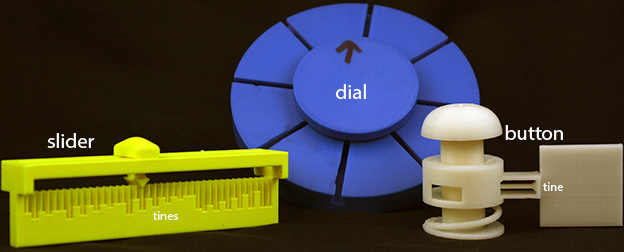
\includegraphics[width=\textwidth]{figures/lamello/fig1-labels-new.jpg}
   \caption{Passive tangible inputs that can be sensed acoustically. %\valkyrie{this one is shorter, which means more space for words! alt one is figures/newfig1.JPG}
   }
   \label{fig:lamello-pretty-components}
\end{figure}

Recognizing mechanically-generated sound for input has important limitations---only movement generates sound, so steady state cannot be sensed---but also appealing characteristics: Components can be fabricated from a single material (e.g., 3D printed ABS plastic), and ``wiring'' only requires attaching a microphone. In this chapter, we offer two important contributions:

\begin{enumerate}
\item a novel sensing mechanism driven by passive, plastic mechanisms that generate predictable sound when manipulated, and
\item design and fabrication guidelines for manufacturing compatible mechanisms, and a demonstration of several traditional input components sensed using our approach
\end{enumerate}

Our evaluation indicates that training-free recognition is possible, though our recognizer only has useful accuracy for a subset of tested tines.

    \subsection{The Geometry-Sensing Link}
    Lamello uses a predictive model which connects the geometry of a cantilevered beam (i.e., the ``tines'' used in this project) to a fundamental frequency when excited. We demonstrate the model, which assumes the beam is uniform, to be useful, in spite of the fact that tines fabricated on a 3D printer are not composed of uniform material. This pre-print modeling of frequencies allows training-free sensing of fabricated input devices using a microphone.
    
\section{Designing with Lamello}

\begin{figure*}[t]
  \centering
    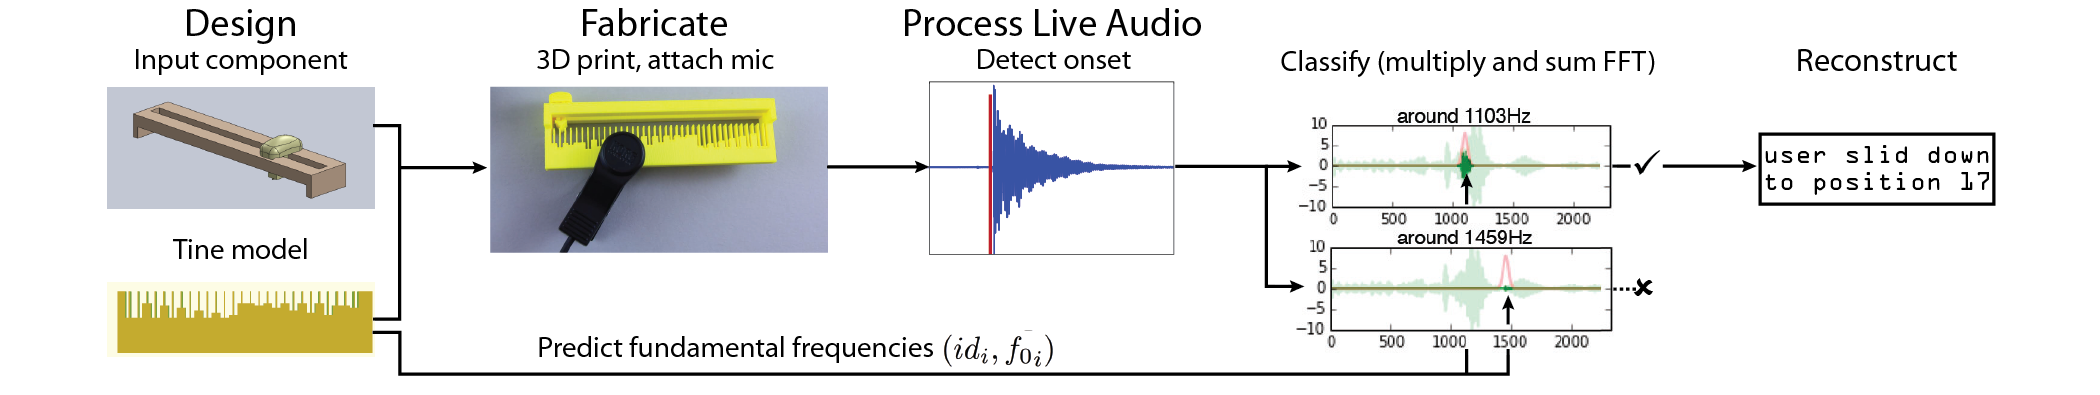
\includegraphics[width=\textwidth]{figures/lamello/systemdiagram-bh.png}
  \caption{Lamello reuses information between the design, fabrication, and audio processing steps to allow training-free passive acoustic sensing.}
  \label{fig:lamello-system}
  \vspace{-0.1in}
\end{figure*}

    \subsection{Users}
    
    Lamello targets makers, who are somewhat familiar with 3D modeling tools (e.g., SolidWorks or Google SketchUp for solid modeling, or openSCAD for programmatic design generation) and 3D printing. In its present, prototype form, Lamello also relies on users' familiarity with basic programming to create software interactions based on user input; it does not leverage record-and-replay as Midas does.
    
    Lamello can generate tine sets automatically; input component geometry---that is, everything that is \emph{not} a tine, like the track and header of a slider---can be derived from its library. The tines and additional geometry must right now be combined by hand. Power users with a more sophisticated understanding of solid modeling programs can generate their own tines by hand (and use Lamello's prediction tools to predict their final frequencies), or create new types of input component geometry to use with their tines.
    
    Once a designer fabricates an input device, the process of preparing it for sensing is simple: he simply places it near a microphone. Users do not need any experience with coding or audio. Lamello automatically predicts the frequencies of tines generated using our scripts, and provides a GUI interface to predict frequencies for hand-built tine geometries. The sensing software only needs the frequency and ordering information from the tines (again, this ordering information is automatically-derived if a user uses our scripts).
    
    To use the output of the sensing tool to control a program, users can either use a record-and-reply style of interaction (for example, using a graphical tool like OSCulator which requires no programming) or accept OSC messages in their own software for more nuanced control.
    
    \subsection{Design Walkthrough}
    
    %\valkyrie{the thing about lamello is that of course it doesn't have a cad tool in the same way. this will be interesting to write.} 
    We discuss the design possibilities of Lamello using a concrete running example: a designer wishes to test out a passive environmental input device for light controls. This input should be in the form of a slider, unpowered, and sensed using a sensor already present in the environment. He has a laptop in his living room to control other aspects of his connected home, so he will use its built-in mic as his sensor.
    
     \subsubsection{Customizing a Library Component}
    The designer opens openSCAD, a free and open source, well-documented CAD tool. He doesn't have much experience with openSCAD, but he opens one of Lamello's library component files: the slider. He needs to be able to input at least 15 different lighting positions, and he wants the slider a bit larger than it is by default, so he changes the values of a few variables in the model. 
    
     \subsubsection{Fabricating Tine-based Components}
    He sends his slider design to a 3D printer for fabrication. His printer is a model which can lay soluble support material, so he simply prints the full design, then performs the necessary post-processing to remove support material. Optionally, for users who don't have access to printers with soluble support, Lamello tines can be lasercut from Polyoxymethylene (Delrin) while only the user-facing mechanism is 3D printed. The two can be assembled afterwards with machine screws and nuts.
    
    \subsubsection{Connecting Hardware to Software}
    
    When his slider comes out of the printer, he sets it on the table next to his laptop and starts the Lamello sensing software, where he enters the material the tines are made of (3D Printed ABS Plastic) to complete the frequency predictions for his model's tines. As he slides the striker past tines, the sound is detected by the microphone in his laptop, which displays an illustration of the slider, with detected tine strikes highlighted.
    
    \begin{figure}
  \centering
    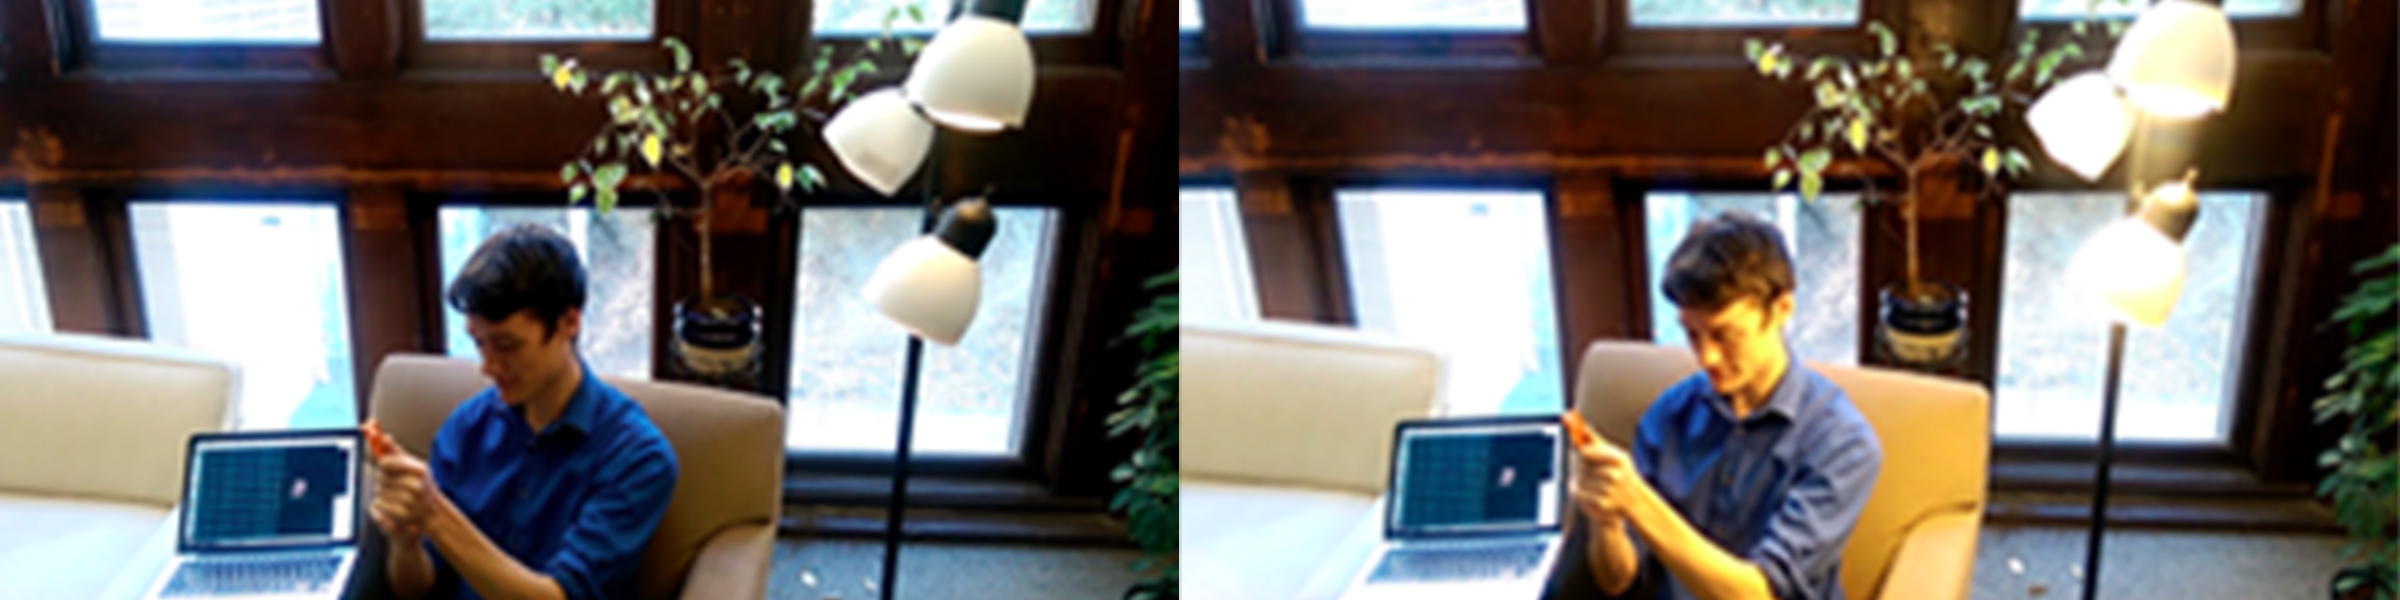
\includegraphics[width=\textwidth]{figures/lamello/andrew-light.png}
  \caption{Our designer tests his lighting setup, holding the printed component in his hand with his laptop and microphone next to him, and observes as the lights change in brightness with each tine strike.} 
  \label{fig:lamello-andrew}
\end{figure}
    
    \subsubsection{Defining Interactions}
    
    To control his lighting system, our designer writes a quick script: he scales the output tine number of his Lamello comb to the input range of luminance for his lightbulb, and forwards those events on to the IP address of the light control bridge. After testing (see Figure \ref{fig:lamello-andrew}), he can affix the Lamello component to the wall nearby the laptop.
    
\section{Implementation}

    \subsection{The Lamello CAD tool}
    
    Lamello relies mainly on just two components: an openSCAD script which generates tine geometry, and a python script which predicts the fundamental frequency ($f_0$) of a tine based on its geometry. These tools can be executed together (the openSCAD script automatically calls the python script) or separately (in the case that a user creates his own tine geometry by hand in another program).
    
        \subsubsection{Tine Geometry Generation}
    
        Through the process of testing and refining our own designs for geometry, we extracted several high-level requirements for tines, described below. These requirements are enshrined in a simple geometry generation script, which we implemented in openSCAD. The script only requires that the user input the number of tines to be generated and the shape in which to generate them: the output is a 3D object which has that many tines of differing fundamental frequencies, which are arranged either linearly or radially. This is accomplished with 

        To generate sounds, we embed tine structures in input components (Figure \ref{fig:lamello-pretty-components}). Our tines are rectangular beams, attached at their base to the component and free to deflect at their top. Interacting with a component causes tine plucks; these vibrate the body of the component and are captured by a contact microphone.
        
        Tines can be arranged in configurations supporting different interactions (e.g., sliding, rotating, pressing).
        
        \subsubsection{Tine Frequency Prediction}

        We model a vibrating tine as an ideal cantilevered beam of uniform density in free vibration~\cite{meirovitch-analytical}: 

            \begin{center}
             $f_0 = \frac{1.875^2 \sqrt{\frac{E\frac{bh^3}{12}}{\rho (bh)L^4}}}{2\pi} \approx .1615 \sqrt{\frac{Eh^2}{\rho L^4}}$Hz
            \end{center}

            Fundamental frequency ($f_0$) is governed by several variables: tine height ($h$) and length ($L$), as well as material properties (density $\rho$, Young's Modulus $E$). Tine breadth ($b$) in fact does not affect final frequency. Our script's generated tine designs keep $b$ and $h$ constant, varying $L$ to achieve different frequencies. This makes the strength required to strike each tine roughly equal: if desired, a designer could make some tines thicker (and thus harder to strike) than others, offering another layer of physical feedback in an interface.

            Our prototypes are 3D printed, resulting in non-uniform material deposition. To test the applicability of our model, we compared predicted and observed $f_0$ for several tines printed on two uPrint SE Plus FDM printers using Stratasys ABSplus-P430 thermoplastic. We find an appropriate material parameter by minimizing the error between observations and measurements. Fitted $E$ values ranged from $9500$ to $15500$ based on print orientation and particular printer. The remaining error $\mu= 69.0Hz$ ($\sigma= 112.5Hz$) shows our model usefully applies to printed tines (see Figure \ref{fig:lamello-freqsgraph}). Estimation of $f_0$ can be further improved by measuring post-print with calipers.
            
            \begin{figure}[b]
 \centering
    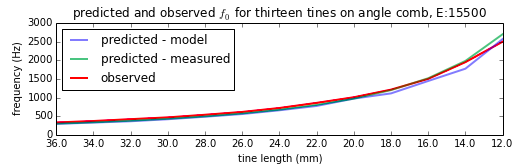
\includegraphics[width=3.25in]{figures/lamello/meirovitch-small.png}
 \caption{Three $f_0$s for tines in one print: predicted from model, predicted from post-print measurements, and observed.  Error, model geometry: $\mu=$ 68Hz $\sigma=$ 36Hz, measured geometry: $\mu=$ 47Hz $\sigma=$ 45Hz.}
 \label{fig:lamello-freqsgraph}
\end{figure}

    This prediction of fundamental frequency can also be run separately on user-entered tine geometries.

        \subsubsection{Information encoding schemes}
        
        We use unique $f_0$s to differentiate buttons and directions on a D-pad. For position sensing, $f_0$ can increase across the range of motion (Figure \ref{fig:lamello-sliders} left). If more distinctions are needed than can be reliably recognized by varying $f_0$, we create de Bruijn patterns~\cite{debruijn-seqproof} (Figure \ref{fig:lamello-sliders} right). A de Bruijn sequence $D(k,n)$ is one which, given an alphabet size $k$ and a subsequence length $n$, contains each subsequence exactly once: we can uniquely infer sequence position from $n$ recognitions. This requires fewer $f_0$s, but more contiguous tine recognitions to determine user input.
        
        \begin{figure}
  \centering
    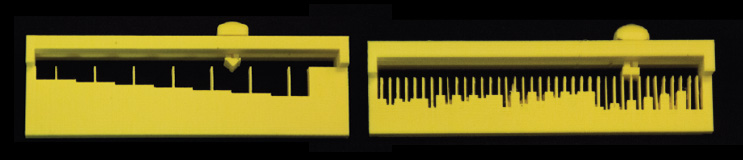
\includegraphics[width=3.25in]{figures/lamello/2sliders-sidebyside.jpg}
  \caption{We experimented with two different encoding mechanisms for sliders: linearly increasing sequences (left) and de Bruijn (right). de Bruijn sequences allow classification of fewer tine lengths, but require more consecutive tine recognitions to determine position and direction.}
  \label{fig:lamello-sliders}
\end{figure}

        \subsubsection{Integration of tines into larger components}

        We augmented several traditional input components: buttons, sliders, dials, and joysticks. Each has a ``striker" attached to the user-facing ``handle'' (Figure \ref{fig:lamello-allcomponents}). These strikers overlap with tine ends by $0.25-1mm$, balancing clear signal generation with easy interaction. Through testing, we determined that a triangular striker profile works best.

        The button has a rib around its shaft that strikes a tine when a user depresses it. The slider has a wiper that overlaps with the tops of tines (tines have different lengths, but are top-aligned). The dial works similarly, arranged radially rather than linearly. The D-pad derives from the button: a striker strikes a tine on the base as the user moves the handle up, down, left, or right.
        
        \begin{figure}
  \centering
    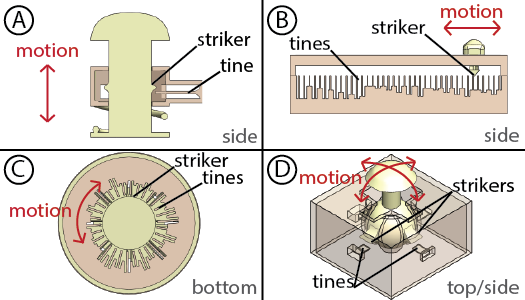
\includegraphics[width=\columnwidth]{figures/lamello/component-schematics.png}
  \caption{The Lamello technique can be used to sense a variety of physical motions, including up/down on a button, back/forward on a slider, and rotation on a dial or scroll wheel.  Four tines used together can sense up, down, left, and right on a direction pad. %\valkyrie{we could cut parts of this figure, given that we never use buttons or joysticks for experiments.  thoughts?}
  }
  \label{fig:lamello-allcomponents}
\end{figure}

        All components we created are parametrically-described models that can be modified to have, for example, more tines on a dial, a longer slider body, or a more robust button spring. Thus, our components can be customized, even without significant experience using 3D modeling software.

    \subsection{The Lamello Hardware}
    
    On the hardware side, Lamello requires both the fabricated input components and the sensing mechanism (i.e., the microphone).
    
    \subsubsection{Lamello's Sensing Apparatus}
    
    Lamello is designed to take advantage of sensors that already exist in an environment, specifically microphones. No custom hardware is necessary to sense Lamello-based inputs. Our initial tests leveraged cheap contact mics used for musical instruments clipped to the components, while we have since performed informal tests with thru-air microphones present in laptop computers. Audio sensing additionally presents more of a challenge, as it necessitates time- and frequency-domain analysis on a device with non-negligible computational ability, unlike the simple thresholded on/off of Midas. We describe our algorithms below.

    The audio signal of a tine strike is characterized by an initial transient---a short high energy sound across a wide range of frequencies---followed by free vibration with a local long-decay energy peak at the tine's resonant frequency (Figure \ref{fig:lamello-transient}). Conceptually, our recognizer detects a transient, finds the dominant resonant frequency after the transient passes, and compares it to predicted tine frequencies.
    
    
\begin{figure}
  \centering
    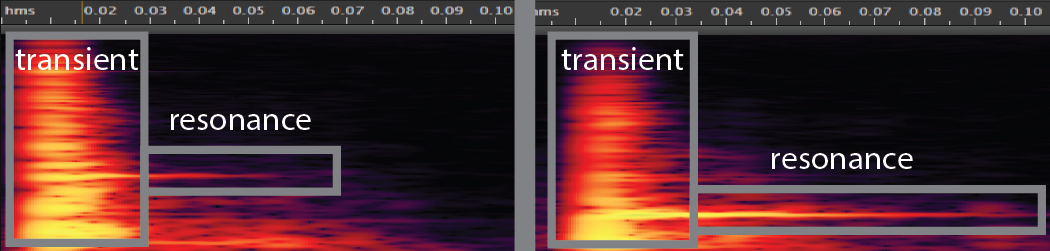
\includegraphics[width=\textwidth]{figures/lamello/transient-resonance.png}
  \caption{Two typical tine strikes (100ms): high-frequency (left) and low-frequency (right).  We mark transients and resonance.  Note the higher frequency has less energy (darker colors) and faster decay (shorter).} 
  \label{fig:lamello-transient}
\end{figure}

    Our audio processing pipeline, written in Python, uses basic frequency-domain features for classification. We sample our contact microphone at $16000Hz$. Our frames (sets of samples captured for analysis) are 2048 samples ($128ms$), and our hop length (offset between successive, overlapping frames) is 800 samples ($50ms$), for a frame overlap of $61$\%. Analyzing a frame takes $5ms$, plus additional latency incurred by sound hardware. In addition to the real-time audio stream, our recognition algorithm also takes an ordered list of $(id_i,{f_0}_i)$ tuples describing the tine ordering and fundamental frequencies of a component as input.

    For each frame, we first determine if a tine strike is present using a standard onset detector (with an empirically-determined amplitude threshold). Once an onset is detected, we wait 2 frame hops for the transient response to pass.
    
    We classify the subsequent frame (computation time: $5ms$). Our best-case onset-to-classification latency is therefore $2 * 50ms + 5ms = 105ms$.  In practice, we have seen latency of $107.3ms$ ($\sigma$=$9.67ms$). Our sound card and the \emph{PySoundCard} driver introduce latency as they collect and report blocks: one could reduce overhead with optimized sound drivers and sample block sizes.

    To classify, we compute a Fast Fourier Transform on the window, then normalize the FFT bin values, such that they represent fractions of overall audio energy. For each possible tine $id_i$, we generate a new measure: the dot product of the scaled FFT and a Gaussian centered at the bin for ${f_0}_i$, which represents the fraction of audio energy $e_i$ in the neighborhood of ${f_0}_i$. To account for lower energy at higher frequencies, we use a scaling factor proportional to the frequency and a $\sigma$ for the Gaussians empirically determined per component, giving an adjusted list of ${e_i}_{adj}$. 

    Mapping a recognized tine identity $id_R=argmax({e_i}_{adj})$ to user actions is straightforward. For buttons and joysticks, $id_R$ maps directly to a discrete input (press, up, down, left, or right). Similarly, for dials and sliders that encode position with linearly increasing tine lengths, $id_R$ maps to a unique position. For dials and sliders that use a de Bruijn sequence $D(k, n)$, we use each sequence of $n$ recognized tines to determine the corresponding position within the sequence (i.e., recognized tines are remembered in order, and this order is compared to the known order of tines on the slider to determine a user's position). For buttons and joysticks, $id_R=argmax(p_R)$ maps these tine probabilities directly to a discrete input event (press, up, down, left, or right), while for sliders and dials the recognized tine, history, and layout are considered in order to generate a progress event ($14\%$, $58\%$, etc.).

    \subsubsection{Fabricating Lamello-compatible Components}
    
    As mentioned, most of our prototype Lamello tines are 3D printed in FFF-extruded ABS plastic. While our $f_0$ predictive model works sufficiently well in spite of the non-uniformity of the material, tines printed in some orientations may break (see Figure \ref{fig:lamello-break}), and may need special calibration as their Young's Modulus ($E$) is likely to differ.
    
    \begin{figure}
  \centering
    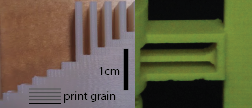
\includegraphics[width=3in]{figures/lamello/fab.png}
  \caption{Tines printed in some orientations may be prone to breaking: in particular, inter-layer adhesion is weaker than within-layer adhesion for 3D printing (left). Breakage can be mitigated by filleting tine corners instead of having them meet the body at right angles (right), but this can require additional details in the frequency prediction model.} 
  \label{fig:lamello-break}
\end{figure}
    
    Other printing or fabrication processes may not be orientation dependent. We have laser cut tines from Polyoxymethylene (Delrin) sheets, integrating these tine strips into 3D printed components using machine screws as fasteners. Tine sizes are similar between ABS-printed and lasercut objects, as laser cutting caused heat deflection in smaller feature sizes. Smaller tine sizes and higher frequencies may be achievable using different fabrication processes, e.g., injection molding or MEMS micromachining. We leave these investigations to future work.
    
    \valkyrie{right now, you're leaving out the entire evaluation section of the original paper. to be fair, that section is about how well the sensing works, rather than how fast/cheap/flexible the technique itself is. however, it likely still needs to go in here. figure out where to put it!}

\section{Evaluation}

    \subsection{Cost-Effective}
    Lamello-based components do not require dedicated sensing hardware: they can be sensed using microphones already present in laptops or, with additional software engineering, in smartphones. Each physical microphone can also be shared among multiple components, as a it need not be physically attached to a single input to acoustically sense it.
    
    The components themselves are also inexpensive, as ABS plastic for 3D printing costs approximately \$$50/kg$, and each of our example inputs weighs roughly an ounce. The polyoxymethylene sheets we experimented with for our laser cutter are approximately \$$10/ft^2$.
    
    \subsection{Fast}
    Input components built using this technique do not require post-processing. The time from design to functioning input is limited mainly by the speed of the 3D printer (while each of our sliders required only 2 hours to print, the joystick took 8). Once the print is completed and the support material removed, the technique does not require training---it relies on $f_0$s predicted from geometry rather than empirically determined---, and the components can be used right away. In the case that designers elect to create their components by assembling lasercut tines with 3D printed mechanisms, the assembly requires simply snapping the tines in (in the case of the dial, see Figure \ref{fig:lamello-laser}, left) or attaching a few screws (for the slider, see Figure \ref{fig:lamello-laser}, right).
    
\begin{figure}
  \centering
    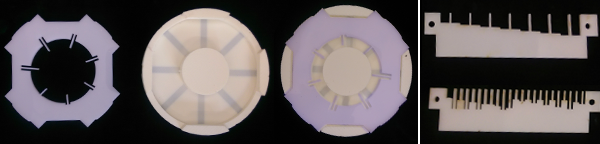
\includegraphics[width=\textwidth]{figures/lamello/lamello-laser.png}
  \caption{Lasercut tines can be integrated with 3D printed bodies. Left, lasercut dial tines can snap into a 3D printed body (lasercut tines are white, blue color added for clarity). Right, lasercut slider tines can be attached with clips or screws through their mounting holes.} 
  \label{fig:lamello-laser}
\end{figure}
    
    In future work, we hope to improve and deploy the Lamello CAD tool to gain insights about its legibility for users.

    \subsection{Flexible}
    We successfully used Lamello to create a variety of input components: buttons, sliders, dials, and joysticks. By combining and modifying their primitive actions (pushing, sliding, turning, and rocking), a designer could employ Lamello to sense components like scroll wheels or direction pads. \valkyrie{how to expand this section? maybe a diagram of how these primitives work and could combine into other input controls.}
    To explore the utility of our technique, we used a Lamello slider and mouse emulation to control a Pong game. The achieved latency was sufficient for simple gameplay; however, Lamello may be better suited to provide input for applications such as volume or lighting control (as described in Design Walkthrough, above), where some latency and occasional misclassified events are acceptable.

\section{Discussion}

Initial experiments with Lamello are encouraging: components augmented with tines are easy to print and use, and tines produce unique, predictable frequencies. However, classification accuracy still needs improvement, and may require a new approach for $f_0>2kHz$.

    \subsection{Sweet Spots}

    Lamello opens opportunities to design tangible, mechanical interfaces cheaply and quickly, without the need to train a machine learning model for sensing. This technique is uniquely suited to creating simple, unpowered inputs in environments where microphones, such as those in laptops or, with additional engineering, cell phones, are already present. This includes applications in the Internet of Things or Smart Home, as we described in the scenario above in \emph{Designing with Lamello}. These inputs can be made more durable or more cheap as required by the application: the same 3D models can be fabricated in a variety of materials as desired.
    
    Like Midas's inputs, Lamello designs can be sized appropriately for the situation: they are not pre-fabricated like sensors for Arduino \cite{arduino} or those used in d.tools \cite{hartmann-dtools}, but rather can be stretched or shrunk or otherwise customized to fit perfectly with a larger design or requirement.
    
    Fabrication of these devices is fast, and they don't require training.
    
    \subsection{Limitations}
    
     We have identified several sources of errors to address in future work:

    \subsubsection{Striker mechanism could be more robust}
    In our experiements, finger-plucked tines had a higher rate of recognition than striker-actuated ones. This suggests that striker-created noise contributes to misclassifications, and future work may explore alternative geometries that create less friction noise.

    \subsubsection{Audio signal attenuates as it travels through component body}
    While microphones placed at opposite ends of a printed slider produce similar overall accuracy, tines are more correctly classified by the closer microphone. Though we could not directly correlate microphone distance and signal RMS energy, this fact suggests that minimizing the distance between a microphone and the tines to be sensed may improve accuracy.

    \subsubsection{Resonance and harmonics interfere with classification}
    Struck tines exhibit an energy peak at the predicted $f_0$, but their frequency spectrum is considerably more complex due to harmonics, component resonance, and other unmodeled material effects (e.g., the layered construction of 3D prints). Competing with non-fundamental vibrations is most problematic for short tines, whose resonant frequencies have lower energy. Future work can also probe optimal frequency distributions to avoid overlap between tine harmonics.

    \subsubsection{Unable to sense static configuration, continuous changes, or directionality}

    The Lamello approach can only detect position \emph{changes}---it cannot sense static configurations as they do not create sound. Continuous inputs are also unfeasible with the tine-based design: individual tines must be struck to localize a user's movement.
    
    We currently also cannot distinguish between the two directions in which a tine can be struck. We believe this could be remedied with ``sided'' tine geometry (i.e., asymmetric tine profiles), however this change would require a more sophisticated predictive model and additional inquiries into suitability for 3D printing.
    
    \subsubsection{Does not support multiple inputs simultaneously}
    Use of thru-air microphones based in laptop, tablets, or smartphones in the place of contact microphones could open applications beyond prototyping (e.g., custom controllers for tablet games). However, filtering out environmental noise collected by thru-air microphones is a challenge, and de-interlacing multiple simultaenous input components (e.g., if a button and slider are activated at the same time) will require more sophisticated signal processing than we have described here.

\chapter{Sauron: Vision-Based Sensing of 3D Printed Mechanisms}

\begin{quote}
[Sauron] was suddenly aware of him, and his Eye piercing all shadows looked across the plain to the door that he had made...

--- J.R.R. Tolkien, \emph{The Return of the King}
\end{quote}

\section{Preamble}

Moving towards even more complex geometry requirements and sensors \valkyrie{obviously change this to match with whatever you end up writing in chapter 2} (well, they seem complex today, but won't seem so in THE FUTURE), we arrive at the Sauron technique, which relies upon mechanical input components (as Lamello did) that are sensed not by sound, but by vision. This enables additional flexibility in design: vision can sense \emph{continuous} changes in components (as opposed to Midas, which relied mainly on discrete inputs, and Lamello, which required separate tine strikes as inputs), and unlike Lamello can sense multiple components at once in its current form---Sauron components are deinterlaced in space rather than Lamello's components which must be deinterlaced in time.

3D printers enable designers and makers to rapidly produce physical models of future products. Today these physical prototypes are mostly {\em passive}. Our research goal is to enable users to turn models produced on commodity 3D printers into interactive objects with a minimum of required assembly or instrumentation. We present Sauron, an embedded machine vision-based system for sensing human input on physical controls like buttons, sliders, and joysticks. With Sauron, designers attach a single camera with integrated ring light to a printed prototype. This camera observes the interior portions of input components to determine their state. In many prototypes, input components may be occluded or outside the viewing frustum of a single camera. We introduce algorithms that generate internal geometry and calculate mirror placements to redirect input motion into the visible camera area.   
To investigate the space of designs that can be built with Sauron along with its limitations, we built prototype devices, evaluated the suitability of existing models for vision sensing, and performed an informal study with three CAD users. While our approach imposes some constraints on device design, results suggest that it is expressive and accessible enough to enable constructing a useful variety of devices.

\section{Introduction}
\valkyrie{How are mechanical interfaces important?  How are they seen today?}

Our environment is replete with products that have dedicated physical user interfaces like game controllers, musical instruments or personal medical devices. While the ubiquity of smart phones has led to a rise in touchscreen applications, retaining physicality has important benefits such as tactile feedback and high performance manipulation~\cite{klemmer-bodies}. For example, gamers prefer physical input for speed and performance, musicians for virtuosity and control.

Rapid additive manufacturing technologies enable designers and makers (we will refer to both groups jointly as ``designers'' for the remainder of this chapter) to quickly turn CAD models of such future devices into tangible prototypes. While such printed form prototypes can convey the {\em look and feel} of a physical device, they are fundamentally passive in that they do not sense or respond to manipulation by a user. Building integrated prototypes that also exhibit interactive {\em behavior} requires adding electronic sensing components and circuitry to the mechanical design. 

Existing research has developed electronic toolkits that lower the threshold of making physical prototypes interactive \cite{arduino, greenberg-phidgets, hartmann-dtools}.
However, such toolkits still require designers to manually assemble printed parts and sensors. Such assembly may also require significant changes to a 3D model (e.g., to add fasteners or split an enclosure into two half shells). Detailed electro-mechanical co-design is time-consuming and cumbersome, and is mismatched with the spirit of rapid prototyping. Alternatively, designers may instrument the environment with motion capture \cite{akaoka-displayobjects} or depth cameras \cite{wilson-depthtouch} to add interactivity, but these approaches limit designers to testing prototypes inside the lab in small, restricted areas.

\begin{figure}
\centering
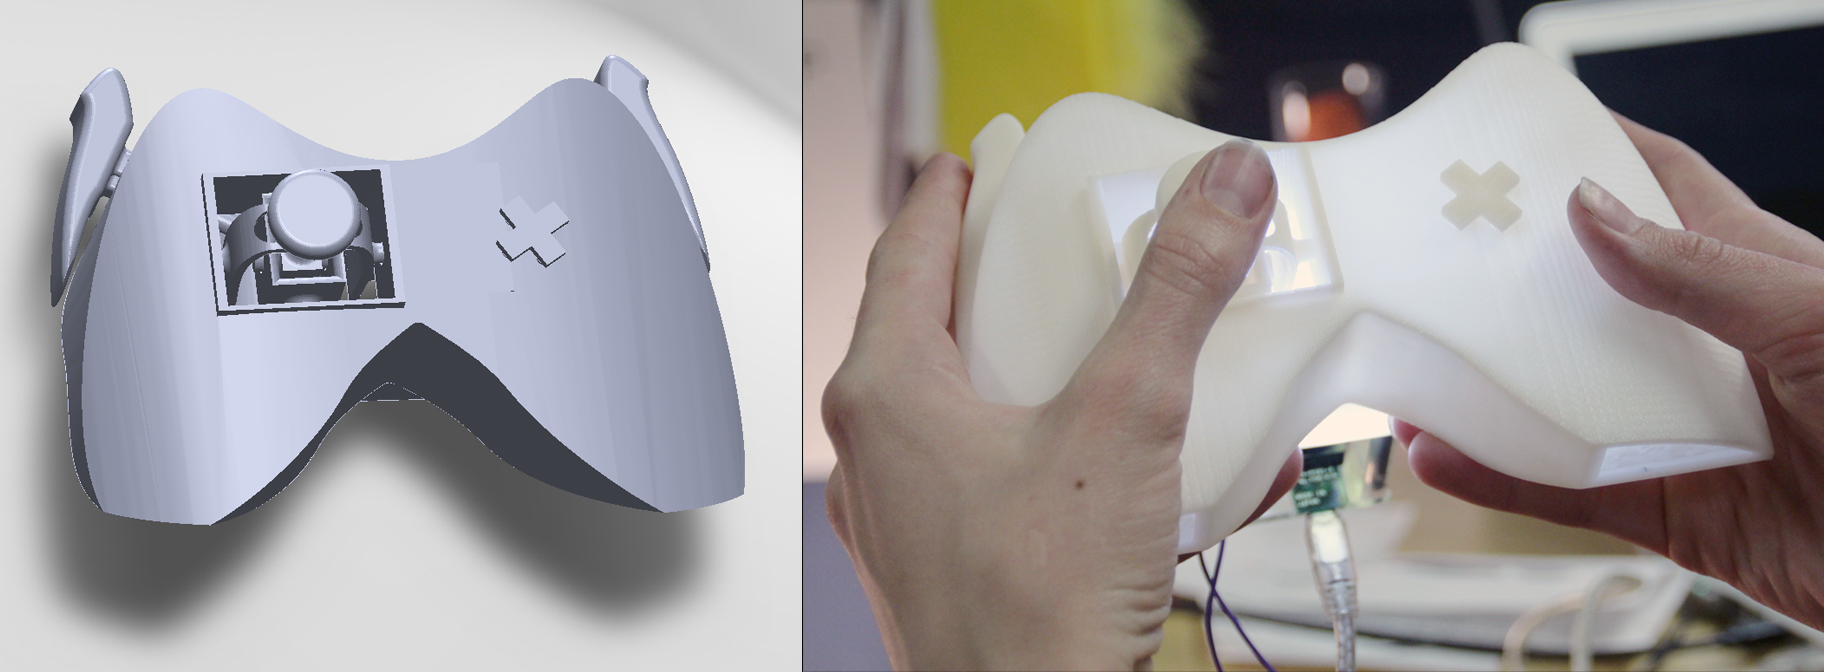
\includegraphics[width=1.0\columnwidth]{figures/sauron/fig1-gamecontroller.jpg}
\caption{With Sauron, designers create a 3D CAD model of an input device and place a virtual camera in the model. Once printed, they attach a matching physical camera to sense user input on the device.}
\label{fig:sauron-teaser}
\end{figure}

Our research goal is to facilitate the creation of \emph{functional} physical interface prototypes on commodity 3D printers with minimal additional instrumentation or assembly (Figure~\ref{fig:sauron-teaser}). In this chapter, we present an embedded machine vision-based approach for sensing human input on 3D-printed physical prototypes. Our system, Sauron, enables designers to 3D print a complete interactive device in a single step. After printing, designers add a miniature camera with integrated ring light to their prototype. After an interactive registration step, Sauron can track the motion and position of buttons, sliders, joysticks, and other input devices through machine vision performed on the user's computer, and forward input events to other applications.

Sensing all input components on a device with complex shape can be challenging, as components may be outside the viewing frustum of a single camera, or blocked by the device's geometry. To address such challenges, we introduce automatic visibility analysis and model modification 
to translate human input into visible movement that can be accurately tracked with standard computer vision algorithms. We first determine which components will be visible to the camera by placing a virtual camera into a CAD model during the design phase. For components that are not visible, Sauron can modify the component model's internal geometry to extend motion into the camera's viewing frustum using parameterized extrusions. Next, Sauron uses raytracing to determine how optical mirrors may be placed to make motion visible in cases where geometry modification fails because of mechanical interference. We implement these techniques by extending commercial parametric CAD software.

While computer vision research traditionally strives to uncover information about an unknown environment, our approach seeks to modify a known environment to facilitate computer vision. Prior work has demonstrated how 3D printed mechanisms can be used to detect physical motion with optical sensors~\cite{willis-printedoptics}; we believe we are the first to automatically modify them based on analysis of a 3D design.

Our approach has some important assumptions and limitations: first, we require a 3D printer that can deposit sacrificial support material to print designs with moving parts in a single pass. Most professional machines support this, but few hobbyist machines do today. Second, for printers that cannot deposit multiple colors simultaneously, a user has to perform some manual marking of a printed model with either reflective or dark pigment. Third, our implementation of the CAD plugin can currently only process certain types of hollow models and is not guaranteed to succeed. Fourth, our current model modification techniques only work for a subset of input components. Despite these limitations, Sauron enables construction of a useful variety of devices.

To evaluate the expressivity of our approach, we describe functional prototypes created with Sauron. 
%We also evaluated the performance and robustness of our approach, which yielded a recognition accuracy of XX\% for discrete input events, and a maximum usable event detection rate of YY Hz (determined by our camera frame rate). \bjoern{didn't happen}
Three knowledgable CAD users were asked to %think out loud and 
design DJ mixing boards with our sensing approach in mind. In all cases the users were able to focus on the usability of their prototype interfaces without being impeded by the sensing techniques. We also evaluated ten pre-made models downloaded from the internet and determined that even designers who did not have vision sensing in mind while designing would have been able to use Sauron for their prototypes in seven of ten cases.

Our main contribution is a design tool enabling users to rapidly turn 3D models of input devices into interactive 3D-printed prototypes where a single camera senses input. This comprises three parts:

\begin{enumerate}
\item A method for tracking human input on physical components using a single camera placed inside a hollow object.
\item Two algorithms for analyzing and modifying a 3D model's internal geometry to increase the range of manipulations that can be detected by a single camera.
\item An informal evaluation of Sauron, a system that implements these techniques for models constructed in a professional CAD tool.
%\item An evaluation of our sensing approach's expressivity and of our prototype's capabilities including detection accuracy and speed
\end{enumerate}

%The remainder of this chapter is organized as follows: we present related work, then a description of our approach. We offer details of our initial implementation. We present a collection of prototypes, created by us, to test Sauron's CAD modification capabilities, and the results of an informal user study using Sauron. Finally, we discuss the limitations of Sauron and conclude with directions for future work.

    \subsection{The Geometry-Sensing Link}
    Sauron uses its knowledge of the geometry-sensing link to actively improve its sensing capabilities. While Lamello and Midas exploited their links to avoid training for completed objects, the Sauron prototype modifies the interior (i.e., non-user-facing) parts of an object to ensure it is compatible with our single-camera sensing technique.

\section{Designing with Sauron}

    \subsection{Users}
    
    Sauron targets mechanical engineers and other users comfortable with physical/product/industrial design and with 3D modeling, but who may not have proficiency in sensing design or programming. Our prototype is built to interact with a specific professional CAD tool, but the techniques described in this chapter could realistically be implemented to work with any of a number of modeling tools (e.g., openSCAD, Rhino).

    \subsection{Design Walkthrough}
    We will describe the process of designing and fabricating models for single-camera sensing with a running example: a designer wishes to prototype a new video game controller with buttons, a joystick, and a direction pad. She wants to explore ergonomics -- how the controller feels to hold and how it will feel during gameplay. She follows the steps in Figure \ref{fig:sauron-step-by-step}.
    
    
\begin{figure}
\centering
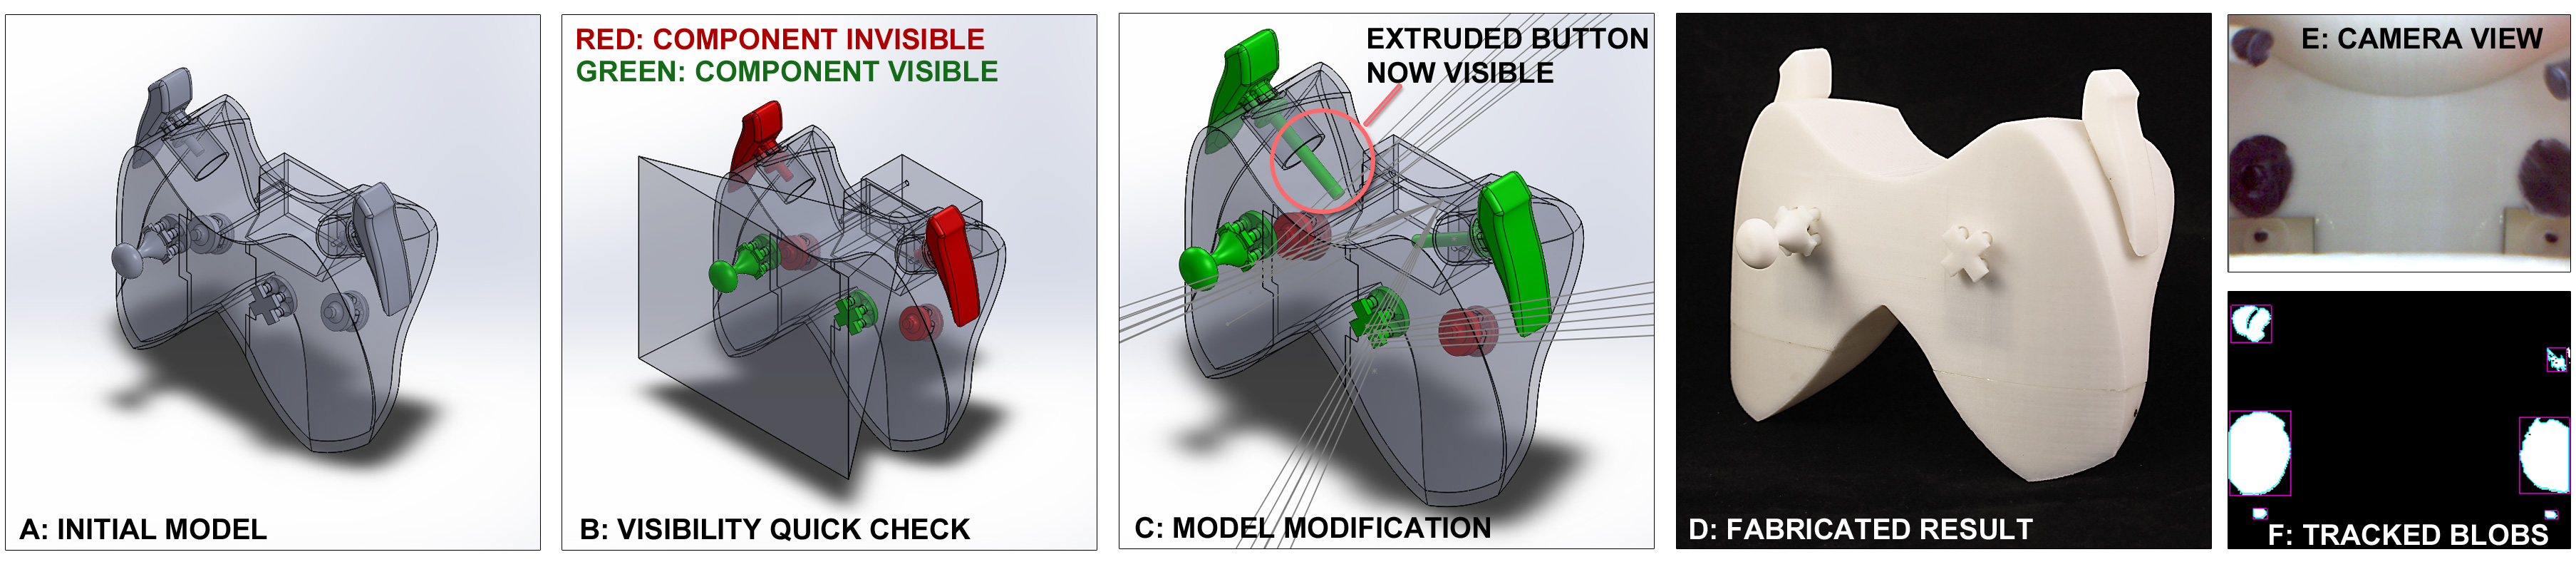
\includegraphics[width=\textwidth]{figures/sauron/fig2-process.jpg}
\caption{When designing with Sauron, a designer begins with his model (A), then inserts a virtual camera and runs quick check for visibility (B).  A full model modification pass (C) performs extrusions and suggests mirror placement to bring invisible controls into the camera's view.  He fabricates his design (D), then colors the inside and inserts the camera and mirrors (E).  The computer vision software tracks the motion of components (F) and forwards events on to control software, such as a game.}
\label{fig:sauron-step-by-step}
\end{figure}


\subsubsection{Modeling} The designer creates a 3D model of her controller in a CAD tool like SolidWorks, placing buttons and joysticks from a library of available controls Sauron provides (Figure \ref{fig:sauron-step-by-step}A). Each library element is parameterized and customizable.

\subsubsection{Adding a virtual camera} Using the Sauron CAD plug-in, she adds a 3D model of Sauron's camera to his assembly. This camera can be positioned anywhere on the model's surface, pointing inwards, into the interior of the hollow model. The designer then adds mount points for the camera so it can be attached with screws once she fabricates her controller.

\subsubsection{Visibility analysis} Sauron provides a ``quick check'' feature which allows the designer to quickly determine if components are directly within view of the camera or if they will require model modifications (Figure \ref{fig:sauron-step-by-step}B). %additional processing (extrusion or mirrors). 
In our example, the joystick and direction pad in front of the camera are visible, so they are colored green. The bumper and rear buttons are not: they lie outside the camera's field of view and are marked red. 

\subsubsection{Model modification} To make the remaining components visible to the camera, the Sauron plugin automatically extrudes the interior portion of the bumper buttons to extend into the camera's field of view (Figure \ref{fig:sauron-step-by-step}C). The rear buttons cannot be extended, as the extrusions would intersect the controller's shell. Detecting this interference, Sauron casts rays from the camera into the 3D scene, reflecting them off the interior of the body, and determines locations where placement of two small mirrors will make the rear buttons visible in the camera image. The plugin visualizes these locations to guide the designer during manual assembly.

\subsubsection{Fabrication and assembly} %Sauron then automatically removes the camera model before generating a file of the entire model suitable for fabrication. 
The designer sends her file (without the camera model) to her 3D printer (Figure \ref{fig:sauron-step-by-step}D). Once the print is completed, an automatically generated instruction sheet guides her through the process of marking the interior of input components, e.g., with black marker (Figure \ref{fig:sauron-step-by-step}E). Last, he screws the camera into its mounts. 

\subsubsection{Registration and testing} Finally, the designer registers the components with the vision system one at at time: her CAD tool prompts her which component to move, and she moves each through its full range of motion to configure its component-specific recognizers. The system then tracks each component separately (in Figure \ref{fig:sauron-step-by-step}E \& F, components are: extruded bumper buttons on top; joystick and d-pad in the middle, reflected rear buttons in mirrors below). Once all the components are registered, she is ready to test her controller.
Sauron sends input event data as OpenSoundControl messages, a format that software tools can understand and map to game controller events. Sauron can also deliver events over WebSockets to applications written in HTML and JavaScript.

\section{Implementation}

In this section, we describe Sauron's camera, CAD component architecture, algorithms for modifying internal geometry, and vision pipeline. 


    \subsection{The Sauron CAD tool}
     
     We discuss the key parts of the Sauron CAD tool: simulation and placement of the camera, and the architecture and modification of parametric components.
    

\subsubsection{Physical and Virtual Cameras}
Sauron uses a single camera to sense input on a physical device. In order to determine visibility of input components inside the CAD environment, Sauron uses a virtual camera that matches the physical camera's measurements and optical characteristics. We empirically measured the field of view of the camera with a geometric test pattern, and we then generated model geometry corresponding to this field of view as a reference for designers (Figure \ref{fig:sauron-hardware}).

\begin{figure}
\centering
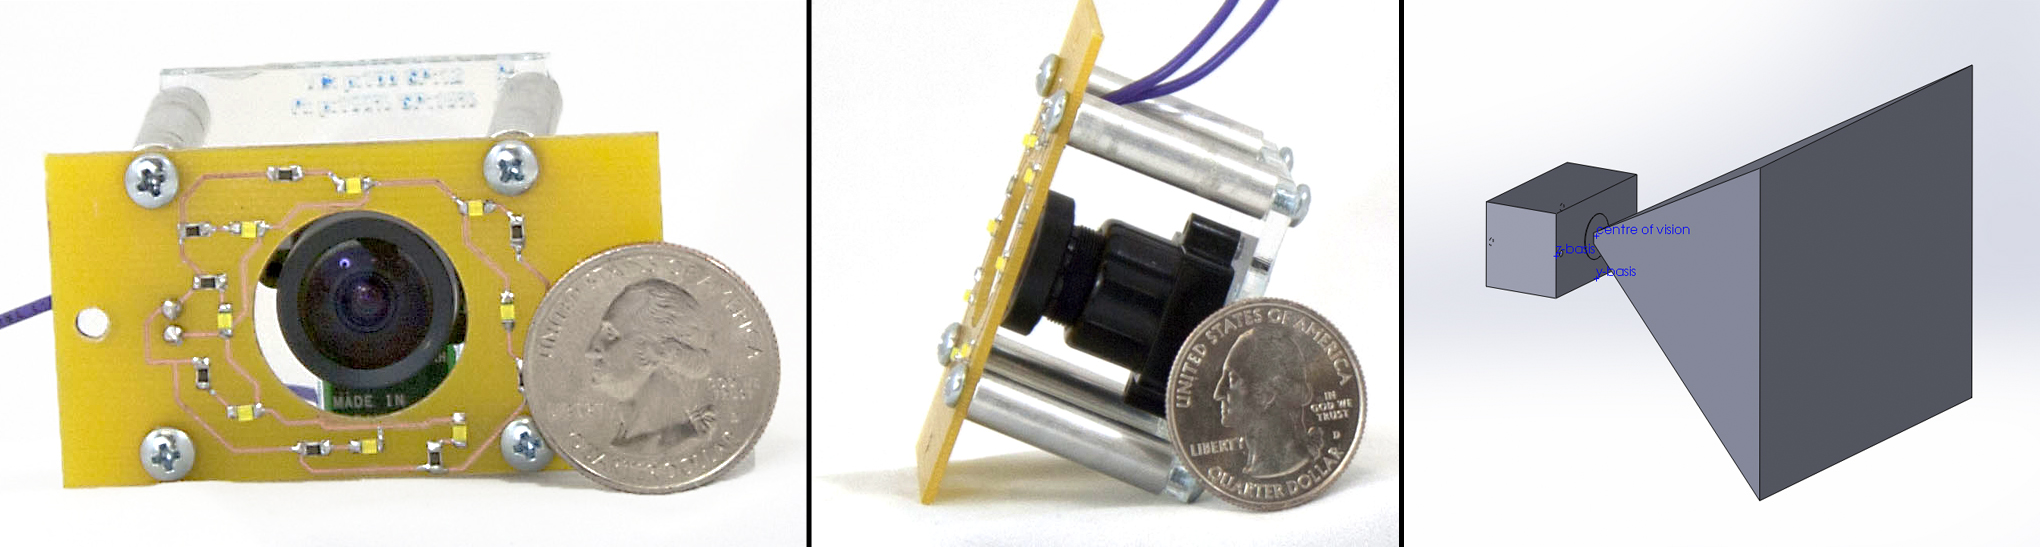
\includegraphics[width=3.25in]{figures/sauron/camera-front-and-side.jpg}
\caption{Left: Sauron's USB camera and ring light.  Right: Our virtual model of the camera and its field of view.}
\label{fig:sauron-hardware}
\vspace{0.2in}
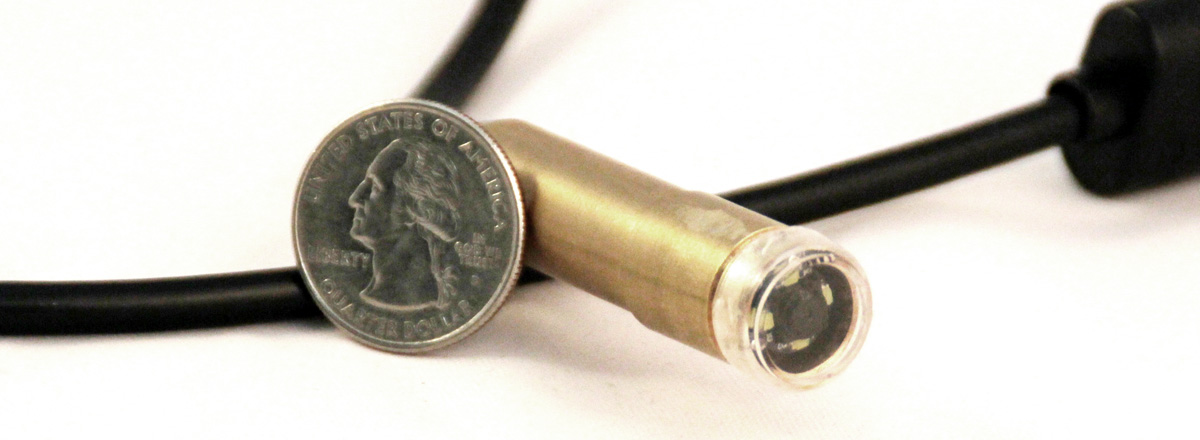
\includegraphics[width=3.25in]{figures/sauron/pipe-camera2.jpg}
\caption{The hardware can be miniaturized, as in this pipe inspection camera with integrated LEDs.}
\label{fig:sauron-inspectioncam}
\end{figure}

Our current implementation uses a 640x480 USB camera with a retrofitted 110 degree M12 lens (Sentech STC-MC36USB-L2.3). The interior of the model is illuminated by a ring light with eight surface-mount white LEDs. This hardware may be too bulky for handheld devices; however, there are no technological barriers to miniaturization. We have also built prototypes using a commercial pipe inspection camera (Figure \ref{fig:sauron-inspectioncam}) which is much smaller, but suffered from a low video frame rate and shallow depth of field .


\subsubsection{Component Library and Architecture }
Sauron provides a library of components with buttons, sliders, scroll wheels, dials, trackballs, direction pads, and joysticks (Figure \ref{fig:sauron-components}). These components, when printed, will be tracked through contrasting material applied in a specific pattern or location. For many of the components, this location is in the base, which is tagged in our models. We require that designers use components with tagged geometry in their devices so our plugin understands which portions need to be visible to the camera as well as how to perform modifications. Our base components are parametric models for the SolidWorks CAD software.

\begin{figure}
\centering
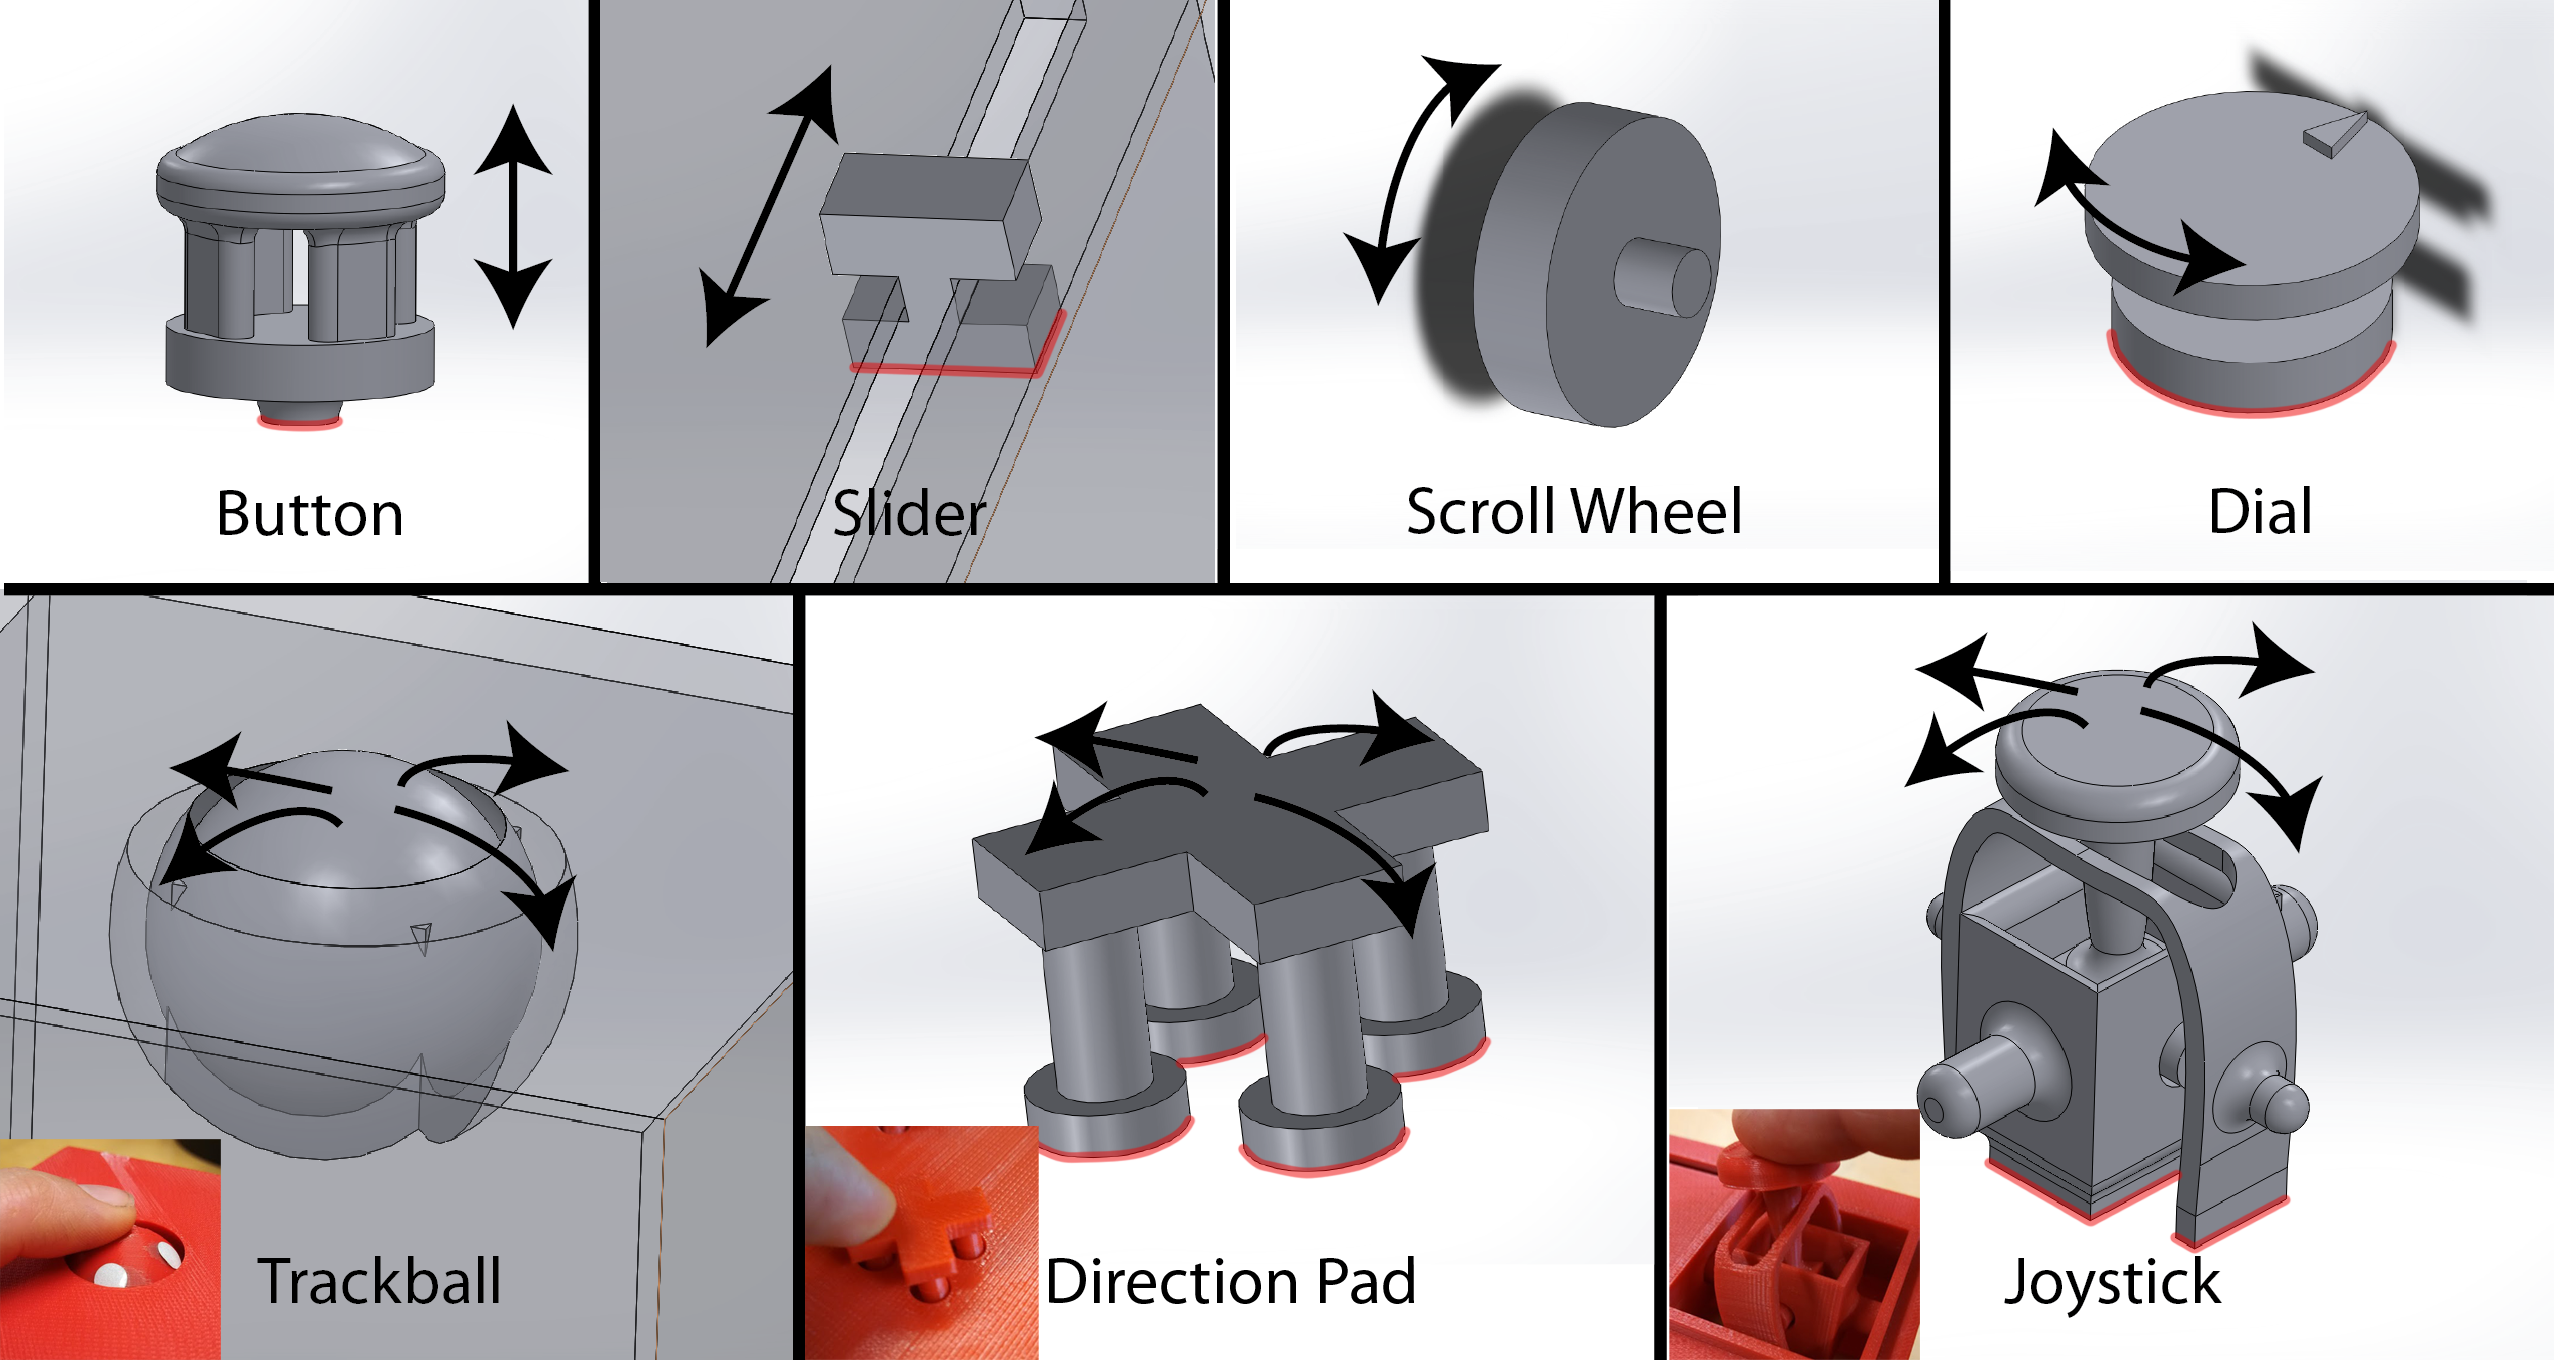
\includegraphics[width=\textwidth]{figures/sauron/sauron-inputs.png}
\caption{Sauron currently supports seven types of input components.  The various components have different types of motion trackable by Sauron, from binary up/down of a button, to one-dimensional slider input, to two-dimensional input from a trackball or joystick.  Extrusion features of components are highlighted in red.}
\label{fig:sauron-components}
\end{figure}

Because Sauron models are parametric, designers already have significant freedom in modifying them to suit their needs. As long as the tagged geometry (on the interior, facing the camera) is kept, the exterior of the models can be changed. As an example, a designer creating a video game controller may make some buttons oblong rather than circular: the long buttons on the side of the controller in Figure \ref{fig:sauron-step-by-step} were built from the same parametric model as the rear circular buttons.

To create a new Sauron-compatible component, the component must exhibit visible motion on the inside of a prototype that can be tracked by the camera. Second, the component must be paired with a suitable vision algorithm to extract its state from visible changes. These two requirements can be decoupled. 
For example, both toggle switches and momentary switches can use the same algorithm extracting a single state bit from a change in position.

\subsubsection{Modifying Components}
Users' CAD models are modified based on an analysis of which input components fall within the field of view of the virtual camera. The two basic modifications our software considers are extrusion and mirror placement. The software which performs model modifications is implemented in C\# as a SolidWorks 2012 plugin. 

\emph{Extrusion}
In order to perform modifications, our initial step is to extend the virtual camera's field of view feature to infinity while maintaining its angles. We revert this after all modification steps are complete. We determine visibility through collision detection between tagged model geometry and the virtual camera's field of view feature.
When components are outside the field of view, e.g., on a side wall (Figure \ref{fig:sauron-extrusion}C), Sauron attempts to extend the component's base through extrusion (Figure \ref{fig:sauron-extrusion}A-B). This technique is not applicable to scroll wheels or trackballs. The model parts Sauron can extrude are shown in red in Figure~\ref{fig:sauron-components}.

\begin{figure}
\centering
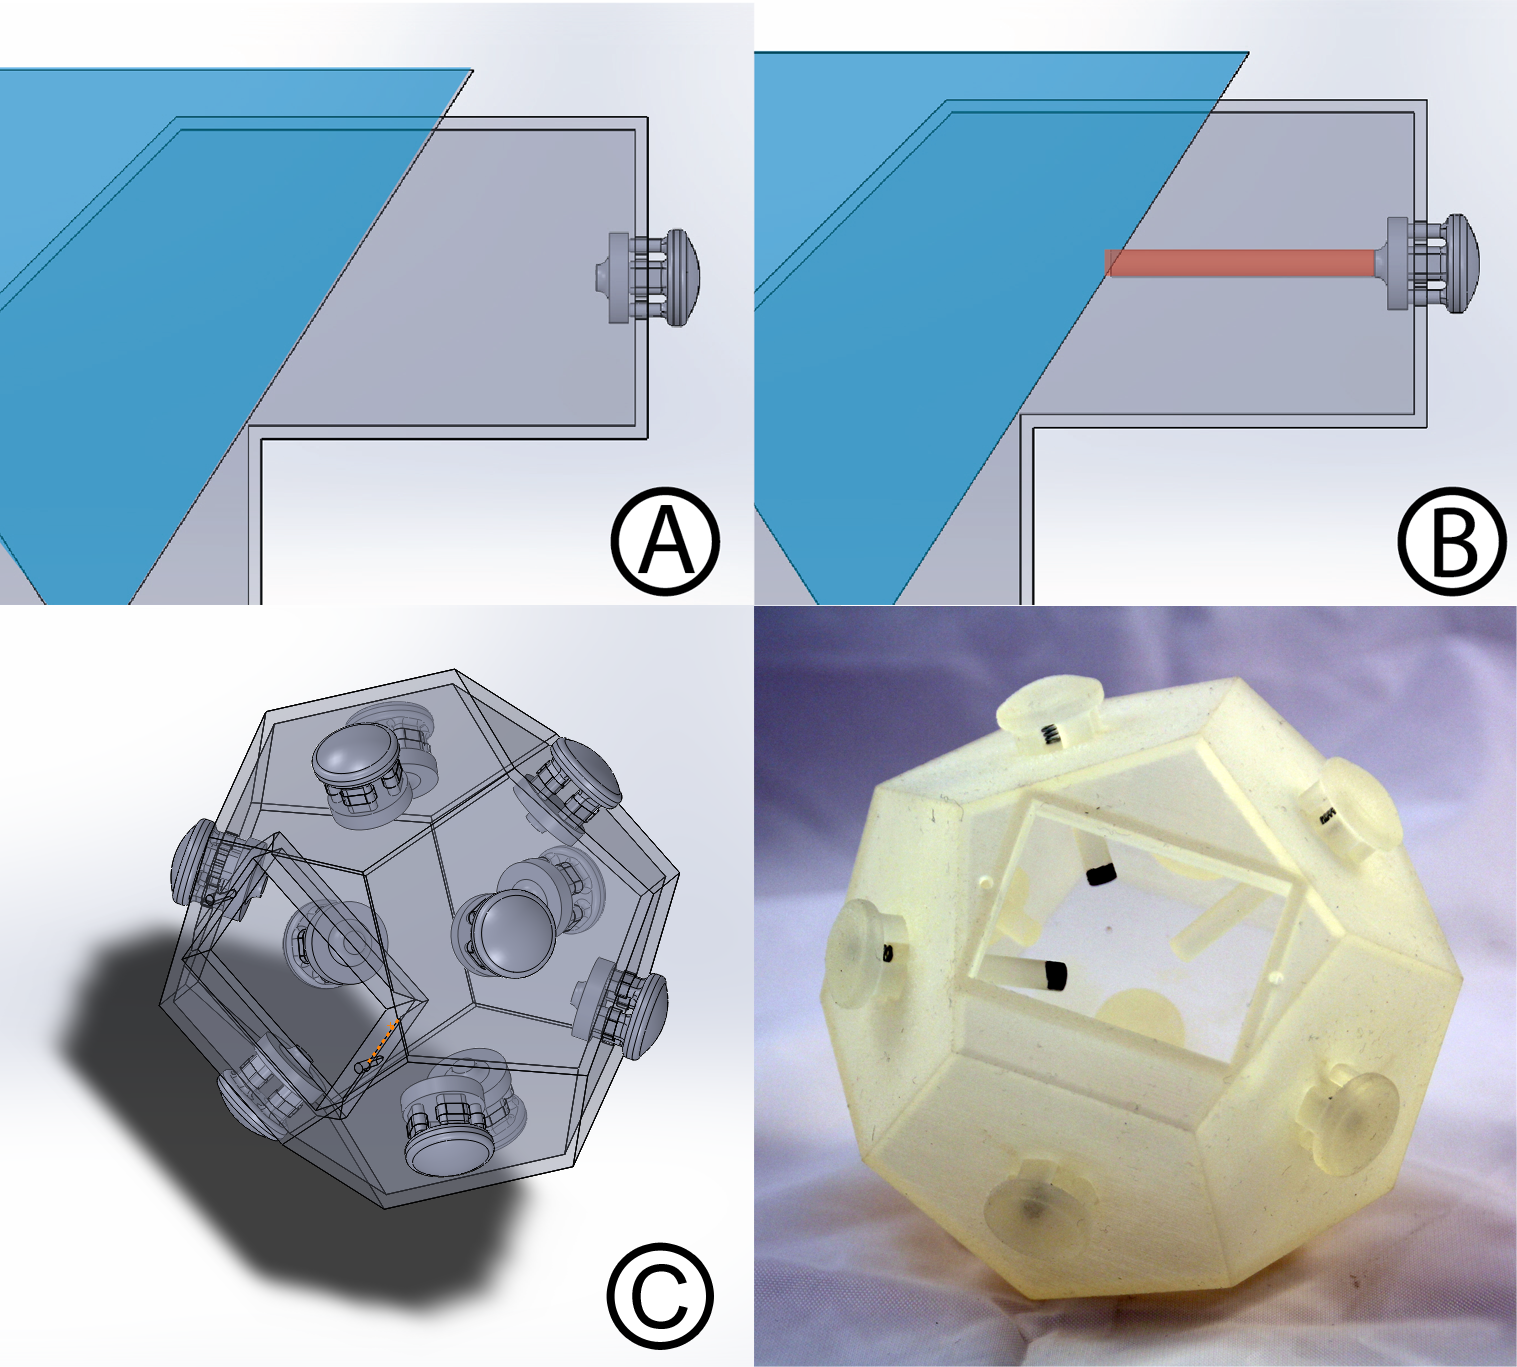
\includegraphics[width=3.25in]{figures/sauron/fig6-extrude-and-dodecahedron.png}
\caption{We measure the distance from the button to the virtual camera's field of view--highlighted in blue (A), then extrude the bottom of the button that distance (B).  This technique is useful when creating objects where input components on many faces point different directions, like this dodecahedral ball of buttons (C).}
\label{fig:sauron-extrusion}
\end{figure}

\begin{figure}
\centering
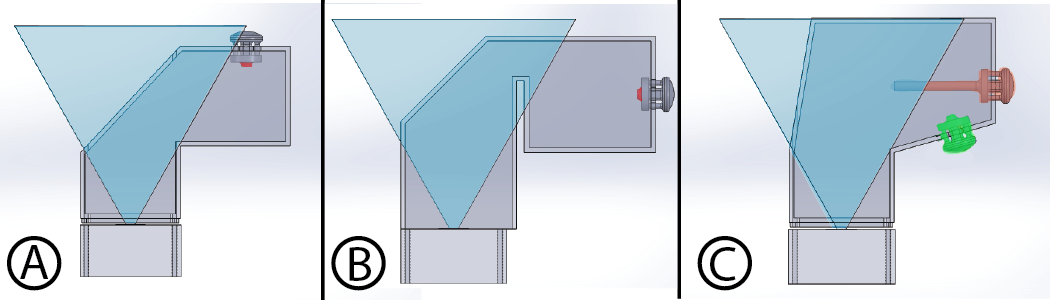
\includegraphics[width=3.25in]{figures/sauron/extrusion-fails.png}
\caption{Extrusion does not work in some cases.  The component's base may not point at the camera's field of view (A).  The component's base may point at the field of view, but be blocked by the main body (B).  One component's base (green), if extruded, would intersect the another component (red) (C).}
\label{fig:sauron-extrusion-fails}
\end{figure}


To calculate extrusion depth, we first cast a ray from the component's base and determine if it intersects the field of view. If not, then we cannot reach the field of view with extrusion. We then measure the distance from the base along its normal to the field of view and update our extrusion to that depth. We next iterate through possible positions of the component (e.g., simulate a slider's motion along its track) and check that we are not intersecting any other components or the body of the device, and that we continue to meet the field of view. We iteratively extend our extrusion if we fall outside the cone and perform mechanical interference checks at all positions at each length. If we avoid collisions, the component has been successfully modified.  Failure cases of this algorithm are shown in Figure \ref{fig:sauron-extrusion-fails}.

Extrusion need not be limited to a single direction straight down from a component's base. We have built proof-of-concept components like the button in Figure \ref{fig:sauron-extrusion-multi}, which have multiple possible extrusion directions. This increases the applicability of extrusion to more complicated geometries. Our prototype does not automatically extrude such components yet, but a designer using the camera's virtual field of view reference can make these modifications manually.

\begin{figure}
\centering
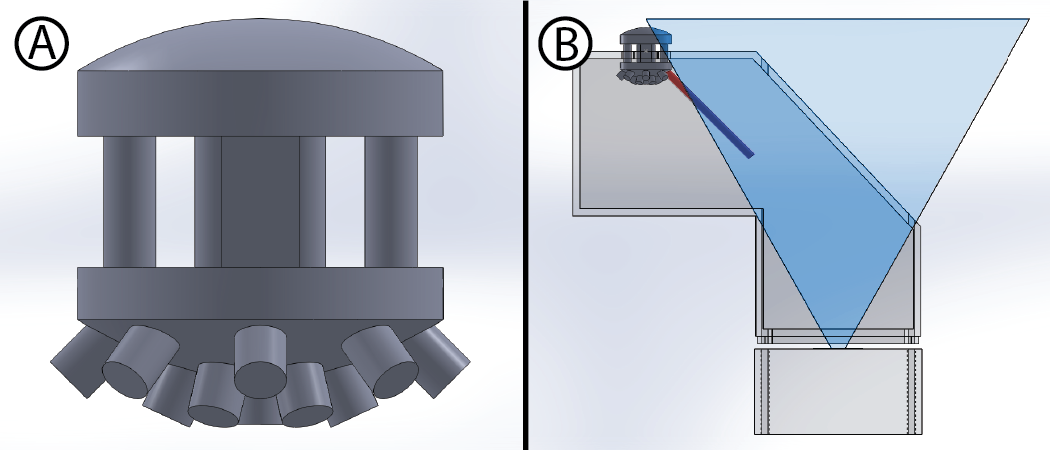
\includegraphics[width=3.25in]{figures/sauron/extrusion++.png}
\caption{This prototype component (A) can be extruded in multiple directions to meet the camera's FOV cone (B). This offers more flexibility than the reflection solution, as it is fully printable without assembly.
}
\label{fig:sauron-extrusion-multi}
\end{figure}


\emph{Visibility Check, Raytracing, and Mirror Placement}
Designers can check visibility of their components by seeing whether they fall within the field of view geometry of the virtual camera. However, the virtual camera's field of view shown to the user has limited depth so it does not interfere with other modeling tasks. Using raycasting, Sauron  provides immediate visibility feedback by highlighting all components that are directly visible to the camera. We cast a ray from the center of the camera to the bottom of each component and determine whether that ray falls inside the field of view. If so, we perform the same check in the maximum and minimum positions of the component (e.g., we slide sliders to each end of their tracks). %In a full simulation we check more positions, but for quick check we find this is sufficient.

We use raytracing to determine how to place mirrors for components where extrusion failed (Figure \ref{fig:sauron-raytracing}). The designer has to manually insert these during post-print assembly. %\bjoern{Redundant?}In cases where a component has been placed around a corner from the camera or is at an angle such that an extrusion would not cause it to meet the field of view cone, simple extrusion of the component's base will not suffice. We use mirrors to provide optical redirection: the mirror reflects light from the camera onto the component's base as well as reflecting the component's motion back to the camera.

\begin{figure}
\centering
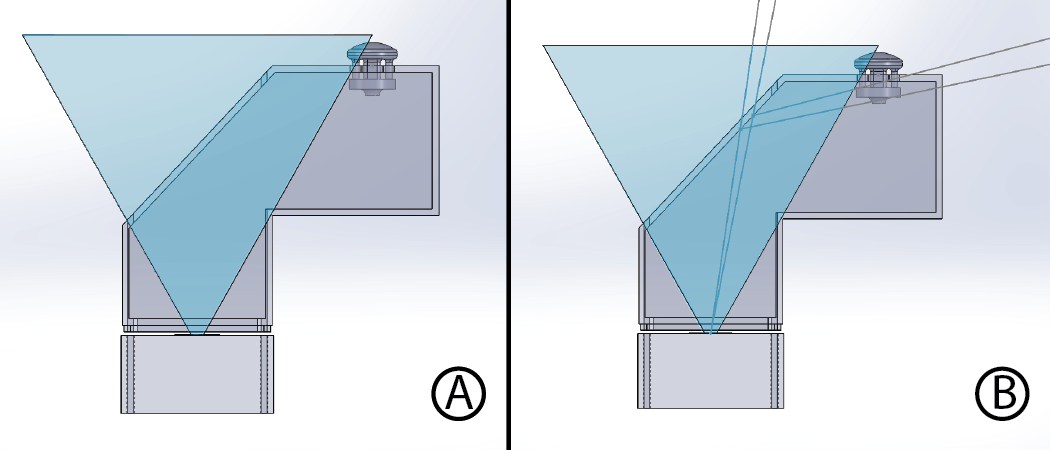
\includegraphics[width=3.25in]{figures/sauron/reflection.png}
\caption{An illustration of the raytracing algorithm used for mirror placement.  Note that the button in the figure cannot be extruded to meet the field of view cone.  A mirror will be glued at the spots where the rays successfully reflect (seen in B) during assembly.}
\label{fig:sauron-raytracing}
\end{figure}

Each ray is cast from the camera to the body of the device, and from there reflected  based on the surface normal of the body at the intersection point: i.e., we assume that during assembly the mirror will be placed tangent to the body's inner face. The reflected rays are traced to determine if they intersect any components which were not successfully modified in the extrusion step. If such a component is encountered by the reflected ray, the location on the body that it was reflected from is marked. This leaves a cloud of points per component, which informs the designer where to place mirrors during assembly (see Figure \ref{fig:sauron-step-by-step}). Our prototype traces a coarse grid of 
20x20 rays because of limitations of the SolidWorks API, in which a single trace takes up to 250ms. A more efficient reimplementation can increase rays to one per camera pixel.

The raytracing algorithm also finds occlusions. If a component %, after being extruded or ``found'' by a mirror, 
is not the first object hit by any direct rays cast or any rays reflected off the main body, the user is alerted that the component needs to be moved or manually modified because it is out of the camera's view. For example, in a case with two buttons in a row and the camera's view parallel to the row, if mirror placement is not possible then the rear button would trigger this alert because all rays cast from the camera hit the front button first.

Mirrors can also be used to redirect motion to increase its visibility. For example, buttons moving along the Z-axis (toward the camera) are harder to track than buttons that move in the XY plane. A 45 degree mirror placed next to the button can redirect visible motion. Our prototype does not automatically calculate the locations of these mirrors yet.

    \subsection{The Sauron Hardware}
    
    We discuss the components of the Sauron hardware: the post-print processing of fabricated input devices, and our computer vision processing pipeline.

\subsubsection{Post-Print Assembly}
Due to the nature of our sensing approach, we require that designers' models be hollow and contain a hole of suitable size for the lighting and camera rig to be inserted. Many prototypes are designed to be hollow because such designs conserve printing material. However, this requirement places some restrictions on how other elements, e.g., an LCD screen, can be placed inside the model. 

We also require a few steps of assembly to make the prototype suitable for use with our vision pipeline.
To increase visibility of the input components versus the background, we require the addition of some distinctive material to the input components. This material can be printed in multi-color 3D printers. Alternatively, coloring the bottoms of the input components with a pen is sufficient. We use a silver permanent pen on dark model material or a black permanent pen on light model material (see Figure \ref{fig:sauron-distinctiveness}).

\begin{figure}
\centering
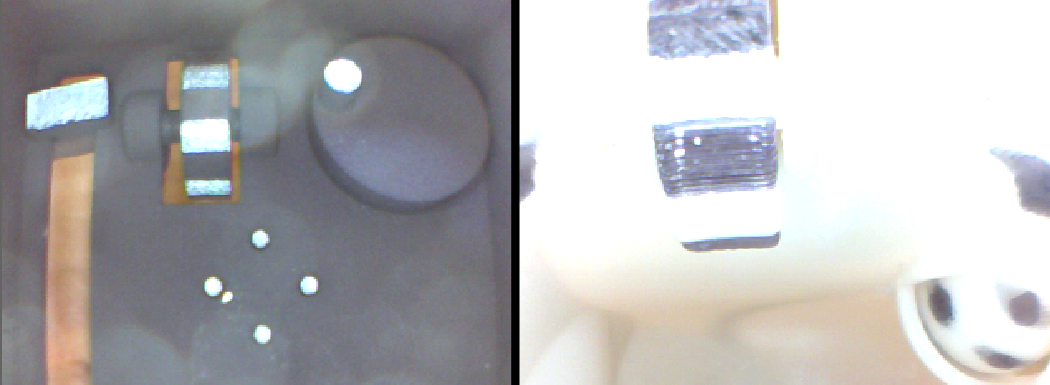
\includegraphics[width=3.25in]{figures/sauron/distinctive-materials.png}
\caption{Components with reflective ink on black material (left) and black ink on white material (right).}
\label{fig:sauron-distinctiveness}
\end{figure}

Because most current materials used for 3D printing are too brittle to create small compliant parts, users must add springs manually after printing (e.g., to restore buttons after being pressed). This limitation is not unique to Sauron. We designed our buttons to allow for insertion of springs using tweezers. Any mirrors will need to be inserted as well. We use small craft mirrors which we affix to the printed device's interior surface with epoxy.

Sauron generates a basic set of step-by-step instructions, automatically displayed in the designer's browser, to assist in correct model assembly. These instructions include automatically-created screenshots of the model highlighting parts that require their attention and example images showing them how to apply mirrors and how to mark components.% for successful sensing.

\subsubsection{Machine Vision}
A computer vision pipeline tracks user manipulations of components once they have been printed.
We run each camera frame through a series of steps: binarization, connected components detection, and previous frame differencing. This highlights movement of components between frames.

\begin{figure}
\centering
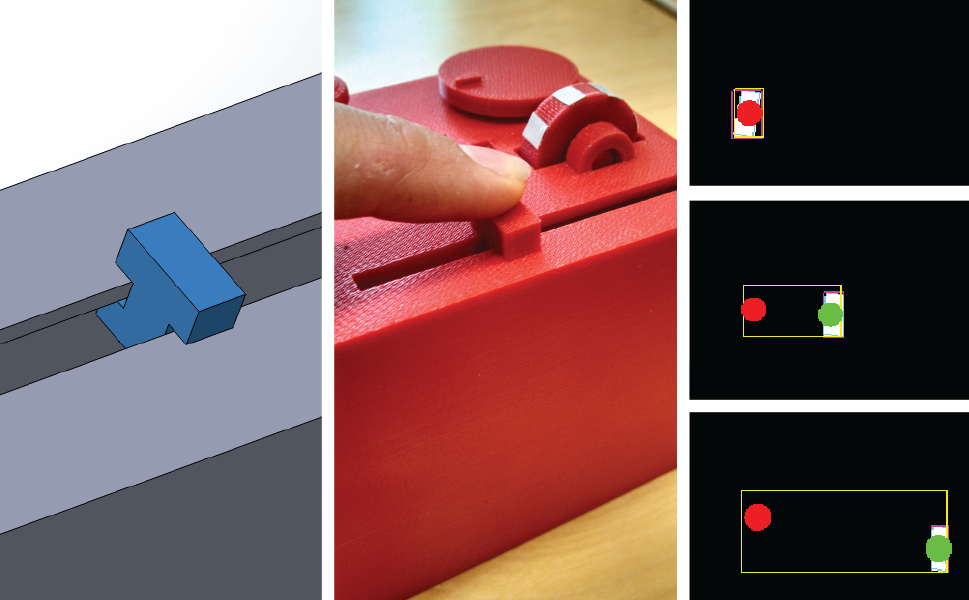
\includegraphics[width=3.25in]{figures/sauron/vision-slider.png}
\caption{Sauron's SolidWorks plugin highlights each model component in turn and asks the designer to move it.  The vision software creates a bounding box as the component moves through its range and also saves any information required by the component type.  For example, to determine slider position later the vision software saves the two most extreme tracked center points (the red and green dots).}
\label{fig:sauron-vision-process}
\end{figure}

\emph{Registration}
Users have to register components before they can be tracked. During the registration process, regions of interest for each component are determined. A designer is prompted by SolidWorks to actuate each of his components in turn, and a bounding region is created that encompasses all the points through which the component moved (Figure \ref{fig:sauron-vision-process}). These regions determine the relative position of the component within its bounds during the testing phase.

In future work, we would like to explore more detailed simulation in the CAD environment. This could eliminate the physical registration phase by either generating and printing visual markers (and using sensing similar to \cite{doering-composition}) in a contrasting material, or by predicting the position of the components in the camera's image and sending that information to the vision software.

\emph{Tracking}
After registration, different detection algorithms apply to each input component. The techniques we use for each component are visualized in Figure \ref{fig:sauron-vision}. For {\em buttons}, we extract one bit of status from movement of its tracked blob. The direction pad generalizes this approach to track four cardinal directions, while the {\em joystick} tracks movement of X and Y axes separately. We find the absolute position of a {\em slider} in a unit interval by finding its blob on a line connecting the minimum and maximum positions observed during calibration (see also Figure \ref{fig:sauron-vision-process}). The {\em dial} tracks position as orientation of a blob around an elliptical path, while {\em scroll wheel} and {\em trackball} use optical flow to determine amount and direction of relative movement.

\begin{figure}
\centering
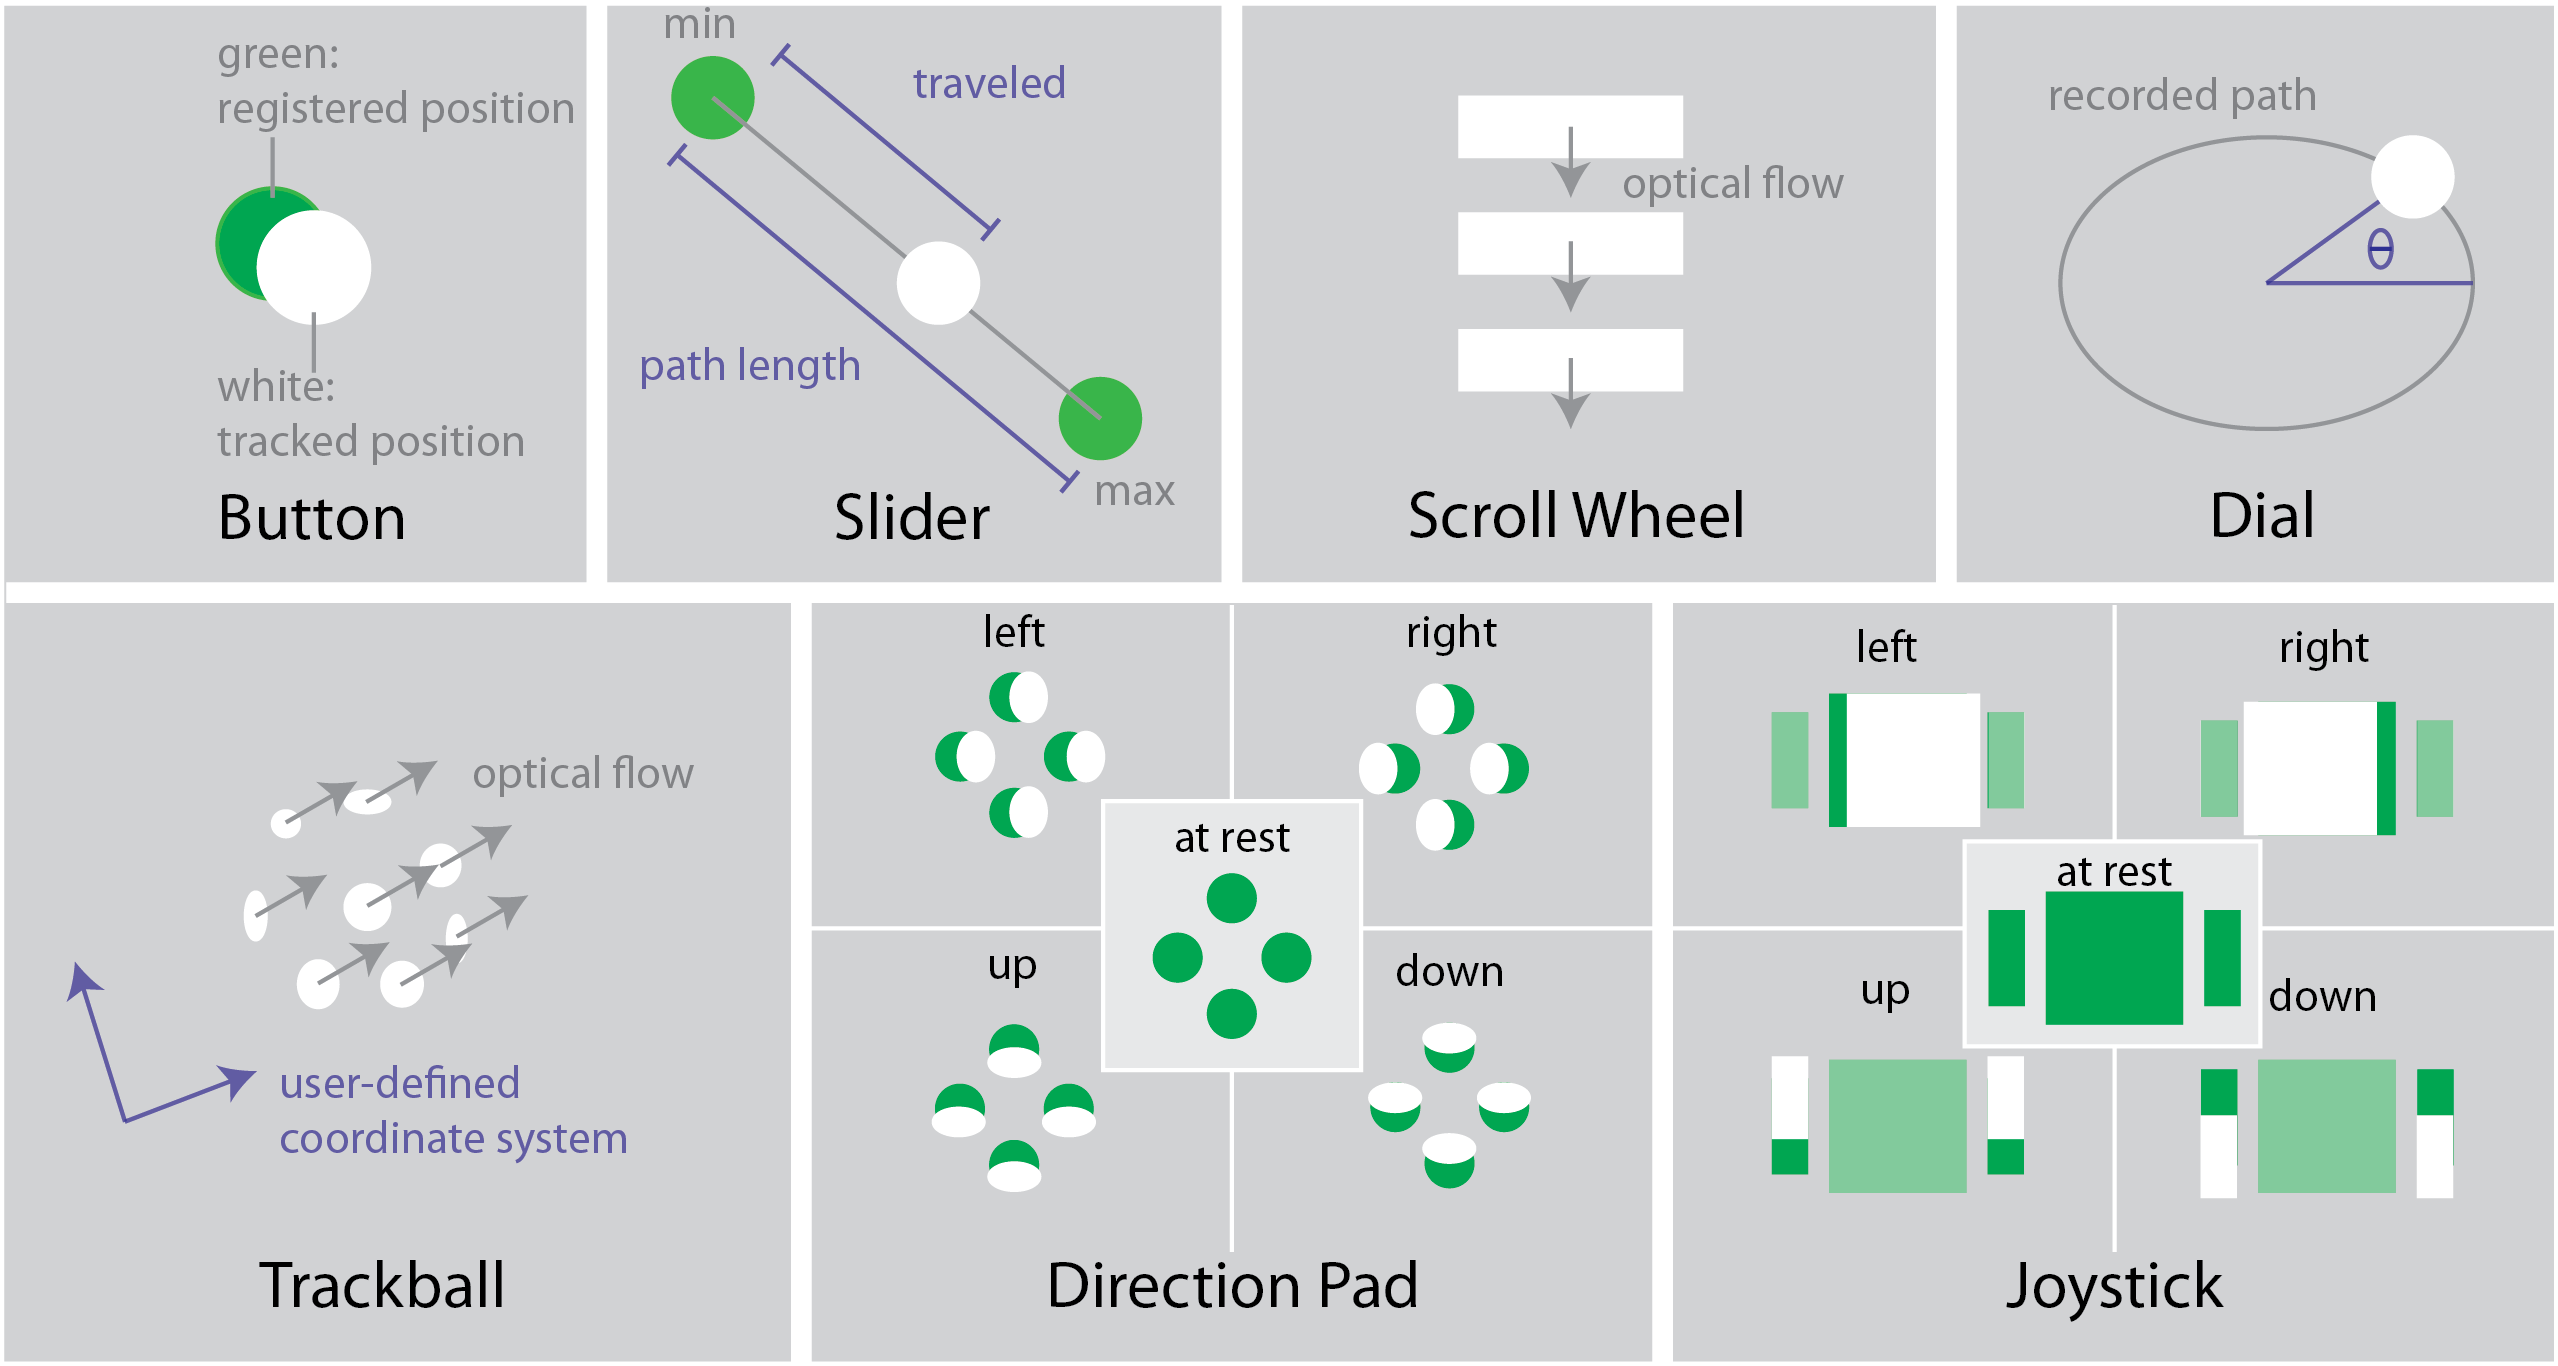
\includegraphics[width=\textwidth]{figures/sauron/vision-all-components.png}
\caption{The different types of components in the Sauron library require tailored computer vision tracking approaches to extract state information.}
\label{fig:sauron-vision}
\end{figure}

We currently do not correct for perspective in our images, which leads to non-linear behaviors in components like the slider and dial. It would be possible to account for perspective analytically since we know position and orientation of a component with respect to the camera in the model. For example, a slider follows a known line through $(x_{min}, y_{min},z_{min})$ and $(x_{max},y_{max},z_{max})$   in the CAD model.
%, and during the registration process a user provides $(u_{min},v_{min}),(u_{max},v_{max})$ for the image of a component in the camera's view. 
Given a slider located at $(u,v)$ in the image, we can find the point that is mutually closest (in a least-squares sense) to the line from the focal point through the image plane at $(u,v)$ and the line of the slider's movement.
% can simply need to solve an inverse projection problem. 
%, or with a more sophisticated raytracing algorithm: if we use our prototype's motion simulation capabilities, we could determine e.g. the bounding box of the slider at all points along its track and share this information with the computer vision software.

The vision component of our prototype is implemented in C++ and runs at interactive speeds (\textgreater 32fps) on a 2011 Macbook Pro. We rely on the open-source computer vision library OpenCV \cite{opencv} and OpenFrameworks \cite{openframeworks}.
%, in particular its support for OpenCV \cite{opencv}. 
Messages are passed between SolidWorks and OpenFrameworks via the OpenSoundControl (OSC) protocol. OSC messages are sent over UDP and contain an address (e.g., {\em ``/button/1''}) and payload (e.g., ``on'' or ``off''). Our prototype uses these messages to communicate processed events, to start and stop test mode, and to start and stop registration of a particular component (see Figure \ref{fig:sauron-arch}).

\begin{figure}
\centering
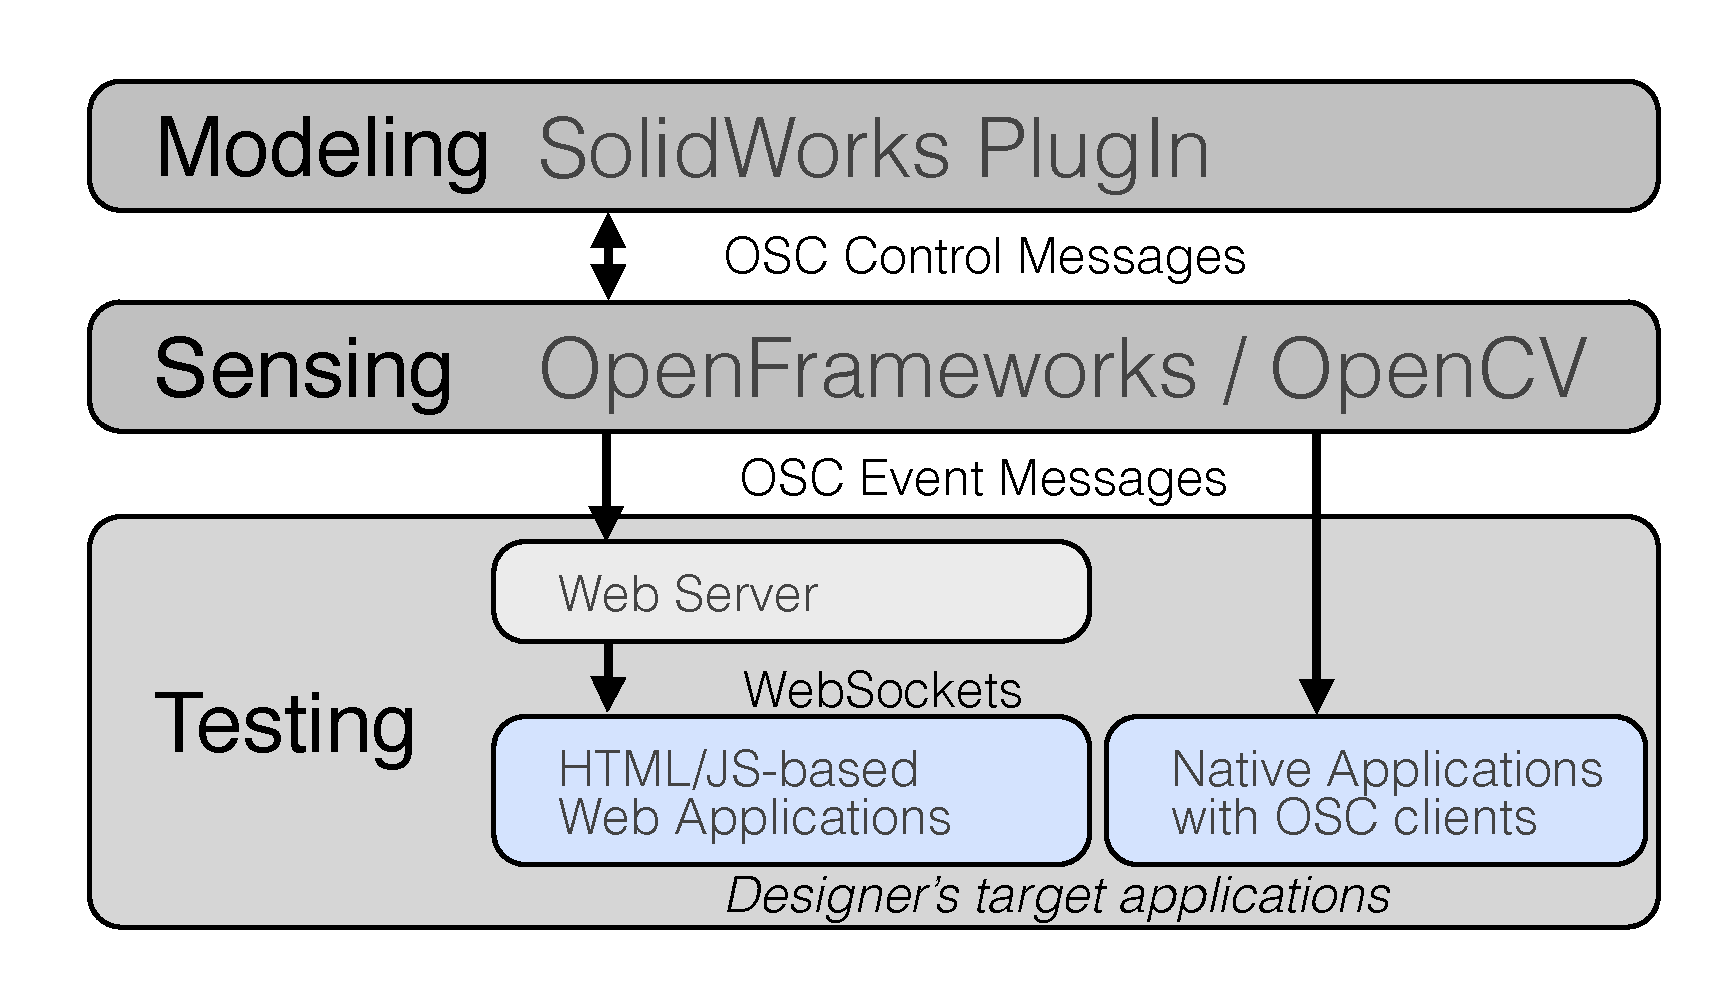
\includegraphics[width=3.25in]{figures/sauron/arch2outlined.pdf}
\caption{SolidWorks and OpenFrameworks exchange messages via OpenSoundControl.  OpenFrameworks also sends OSC messages containing processed data to a WebSockets server to deliver events to a user's application.}
\label{fig:sauron-arch}
\end{figure}

\subsection{Event Output}
Sauron can deliver input events to application using either OpenSoundControl or WebSocket messages.

\subsubsection{OSC messages for simple control}

Existing third-party tools can transform OSC messages into keyboard, mouse, or game controller events, without the need to write code. For example, using the third-party program OSCulator, a designer could simply assign messages coming from {\em /joystick/x} to move the mouse cursor in the X direction and from {\em /joystick/y} to move it in the Y direction. This strategy can also be employed to generate USB HID game controller events and key presses automatically without code.

\subsubsection{WebSocket communication with web applications}

For designers who wish for more control and who are familiar with programming, we enable event consumption in web applications written in HTML and Javascript. Leveraging web applications as a platform allows interface prototyping on any device with an internet-connected web browser. 
We use a node.js server which exposes processed events over WebSockets. We adopt this strategy from Midas~\cite{savage-midas}. 

\section{Evaluation}

In order to demonstrate that Sauron's sensing and fabrication technique fits our criteria of being a cheap, fast, and flexible method of prototyping, we elaborate on each of these criteria below.

    \subsection{Cost-Effective}
    
    Sauron's sensing hardware for our prototype includes a repurposed webcam with a custom circuitboard to hold an integrated ring light: a setup costing roughly \$$35$. Our initial experiments indicate that existing cameras with ring lights (as in Figure \ref{fig:sauron-hardware}) can also be used for sensing, without the need for custom electronics. In addition, a single sensing setup can be used for multiple prototypes, albeit not simultaneously, allowing amortization of cost over many projects.
    
    To work with our computer vision pipeline, prototype objects are hollow. This not only enables our sensing technique, but also saves materials. The fabricated prototypes we used for our research were created on a Stratasys uPrint SEPlus, at the cost of approximately \$$8/in^3$. Today, more and more hobbyist machines are capable of laying down the sacrificial support material that is necessary to create mechanisms in-place that do not require assembly, for roughly \$$50/kg$.
    
    \subsection{Fast}
    
    We performed an informal evaluation with three mechanical engineers. All were proficient SolidWorks users. We first explained how Sauron works and demonstrated a printed prototype containing examples of all our input components. We then asked them to prototype a disk jockey (DJ) controller that could be tested with Sauron. Common functions on such controllers are volume and EQ control knobs, large ``scratch'' wheels for two audio channels, and a crossfader. We emphasized thinking aloud, as we wished to determine how the constraints of our vision-based system affected their design process. Participants did not run the plug-in itself during the modeling sessions due to time constraints, but we ran it on the resulting models and fabricated one of their designs (see Figure \ref{fig:sauron-djmixer}).
    
    \begin{figure}
\centering
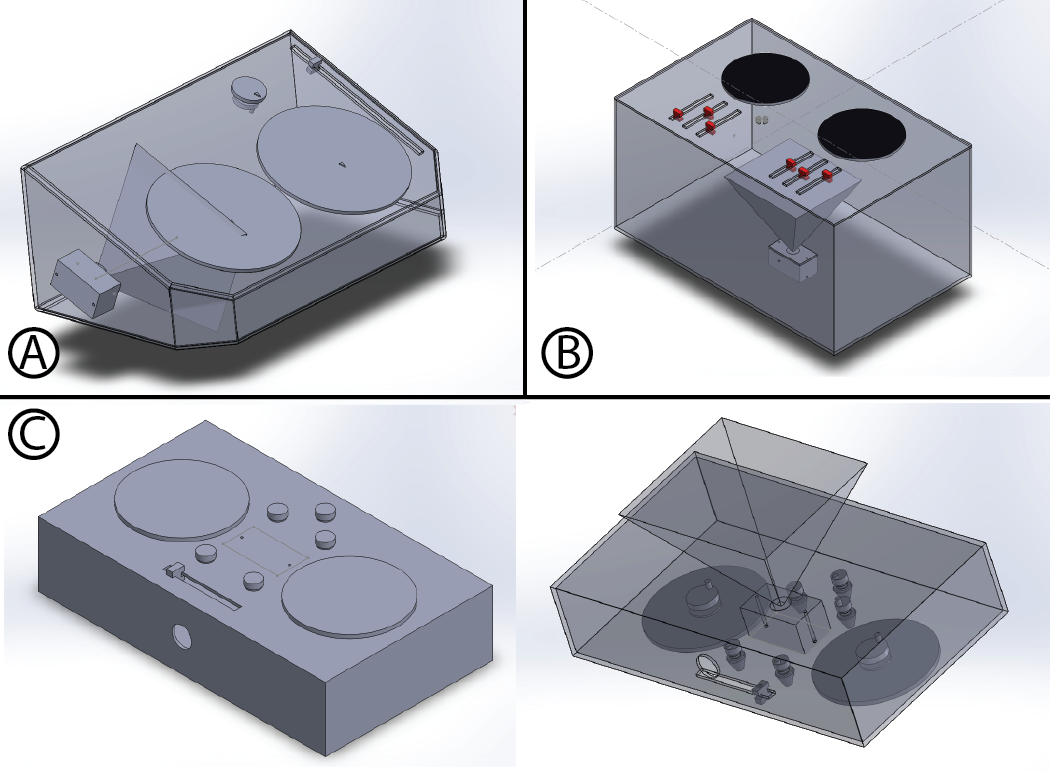
\includegraphics[width=3.25in]{figures/sauron/study.png}
\caption{Our three user study participants prototyped DJ mixing boards using our component library.  Each had a very different strategy for ensuring the camera could see all components.  The assembly on the bottom (with interior cutaway view at right) was designed to have the camera inside reflecting off mirrors placed on the back wall.}
\label{fig:sauron-study}
\end{figure}

    All of our participants modeled DJ mixing boards that could be successfully used with our vision-based sensing approach (Figure~\ref{fig:sauron-study}). They followed different approaches to place the camera -- though all showed concern for the aesthetics of their design and accordingly tried to mount the camera inside the main enclosure or otherwise out of the way. One user mounted the camera sideways (Figure~\ref{fig:sauron-study}A), but at a location such that the mixer's components would not occlude each other; another created a very deep box at the start, stating that he preferred ``to focus on the user side, rather than the camera because I don't care about the box size'' (Figure~\ref{fig:sauron-study}B). The most ingenious design mounted the camera on the top, pointing down, so that all components would be visible in a single large mirror placed at the bottom of the controller (Figure~\ref{fig:sauron-study}C). In aggregate, while users had to plan for the visibility constraints of camera sensing in their design, these constraints were not seen as overly burdensome.

    One user wished that an interactive design checker was available to test his design iteratively for visibility. A complete model modification pass currently requires $\approx 5$ minutes to process a non-rectilinear model with 10 components, because of slow calls to the SolidWorks API. Based on this feedback we implemented the ``quick check'' feature which highlights components that are immediately within the viewing area without performing ray-tracing or extrusion.

    Participants also successfully modified the library of parameterized components. One participant stated that it was important to her that the sensing portion of each component was decoupled from the user-facing portion. For example, the scratch wheels are large on the user's side to enable users to place their entire hand on them, while the internal dial diameter is small so it can be seen by the camera in its entirety (see Figure \ref{fig:sauron-study}C). The same user also wished that there was better documentation for the component library, describing how large holes for mounting needed to be.


    \subsection{Flexible}
    
    To determine if Sauron allows sufficient design freedom for users, we performed an analysis of models created without our approach in mind, as well as modeled and processed several objects ourselves.
    
    \subsection{Analysis of Pre-Designed Models}
    To determine if designers working without our constraints in mind would create prototypes that are compatible with our vision-based system, we downloaded several online 3D models and analyzed them. The models, which comprised a deduplicated set of all models with keywords ``interactive'' or ``controller'' on the model-sharing site grabCAD.com, ranged from XBOX and Guitar Hero controllers to interactive desks with keyboards. None of the devices that we analyzed were designed for 3D printing, but rather for rendering or as engineering drawings.  Our first step in processing them was estimation of the internal geometry of the bodies, for which we assumed simple shelling (i.e., no internal supports, wall thickness approximately .1'', interior curves following the curves of the outside of the body). After this was done, we selected several candidate camera locations which would not interfere with what we understood to be the user-facing functions of the device, and we measured which components would be visible to the camera directly, which via extrusion, and which via reflection. 
    
    \begin{figure}
\centering
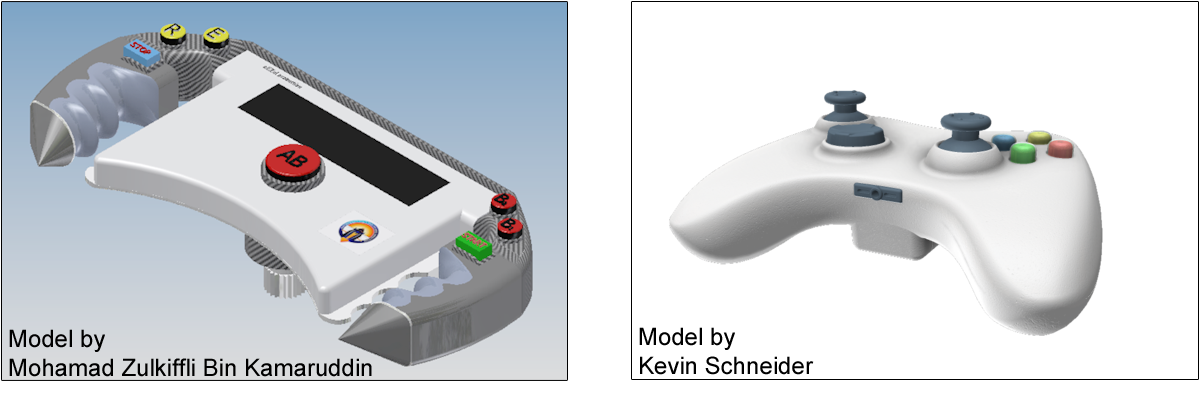
\includegraphics[width=3.25in]{figures/sauron/shallow-models.png}
\caption{These models found online were too shallow to sense with Sauron---occlusion and curvature would prevent correct sensing with computer vision.}
\label{fig:sauron-premade}
\end{figure}

    Out of 10 devices we analyzed, we believe that 7 of them could be successfully processed by Sauron. Three devices were too thin---this caused serious occlusion problems between components. Their bodies also did not allow space for the inclusion of mirrors to solve the occlusion problem (Figure \ref{fig:sauron-premade}). One of the failing devices, a steering-wheel-style device, had two handle areas with buttons at their far ends and thin, continuously-curving surfaces bending away from the main body. Using just one mirror bounce, it would be impossible to see around these bends to the buttons at the ends.


    \subsection{Example Devices}
    We also fabricated three prototypes that display the range of interactive components our prototype system offers.

        \subsubsection{Ergonomic Mouse}
        Our ergonomic mouse (see Figure \ref{fig:sauron-ergomouse}) has a trackball the user can manipulate with his thumb as well as two buttons and a scroll wheel. We configured the mouse to control the mouse cursor on a laptop using OSCulator. Due to large tolerances in our model, the scroll wheel tended to oscillate between ``up'' and ``down'' states after being released. This problem could either be addressed through modifications to the model or by double thresholding in our computer vision component.
        
        
\begin{figure}
\centering
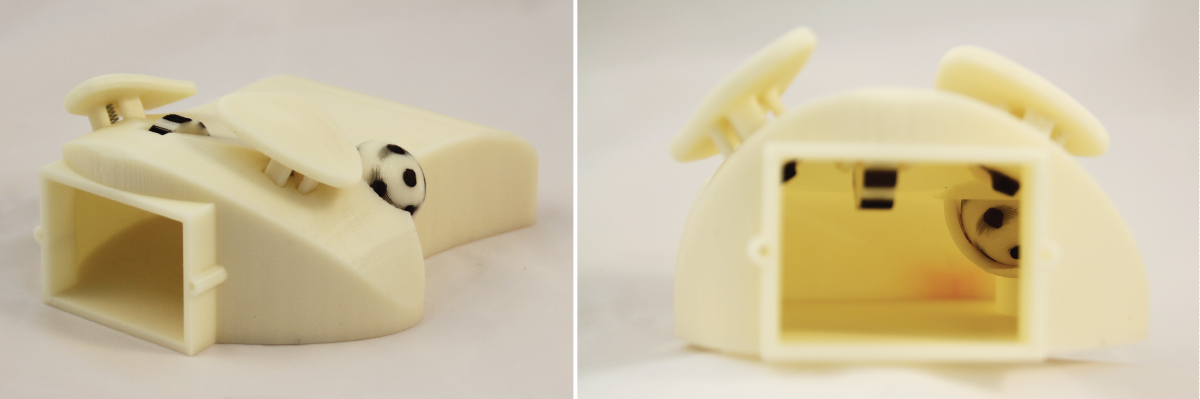
\includegraphics[width=3.25in]{figures/sauron/ergomouse.png}
\caption{Our ergonomic mouse prototype has a trackball the user can manipulate with his thumb as well as two buttons and a scroll wheel. On the right is the camera's view of the inside of the mouse.}
\label{fig:sauron-ergomouse}
\end{figure}

        \subsubsection{DJ Mixer}
        We constructed a DJ mixing board---based on a study participant's design---in two pieces to fit on our 3D printer's bed size. We converted the OSC messages sent out by Sauron's vision software to MIDI messages to control Traktor, a professional DJ application (see Figure \ref{fig:sauron-djmixer}). One issue this prototype raised was that disparities between the virtual and physical camera parameters affected visibility. While the components were designed to fit within the virtual camera's field of view, an offset between the lens axis and the center of the sensor on our (manually-modified) camera led to some components falling outside the physical field of view. We are confident that better calibration and measurement can overcome such problems.
        
        \begin{figure}
\centering
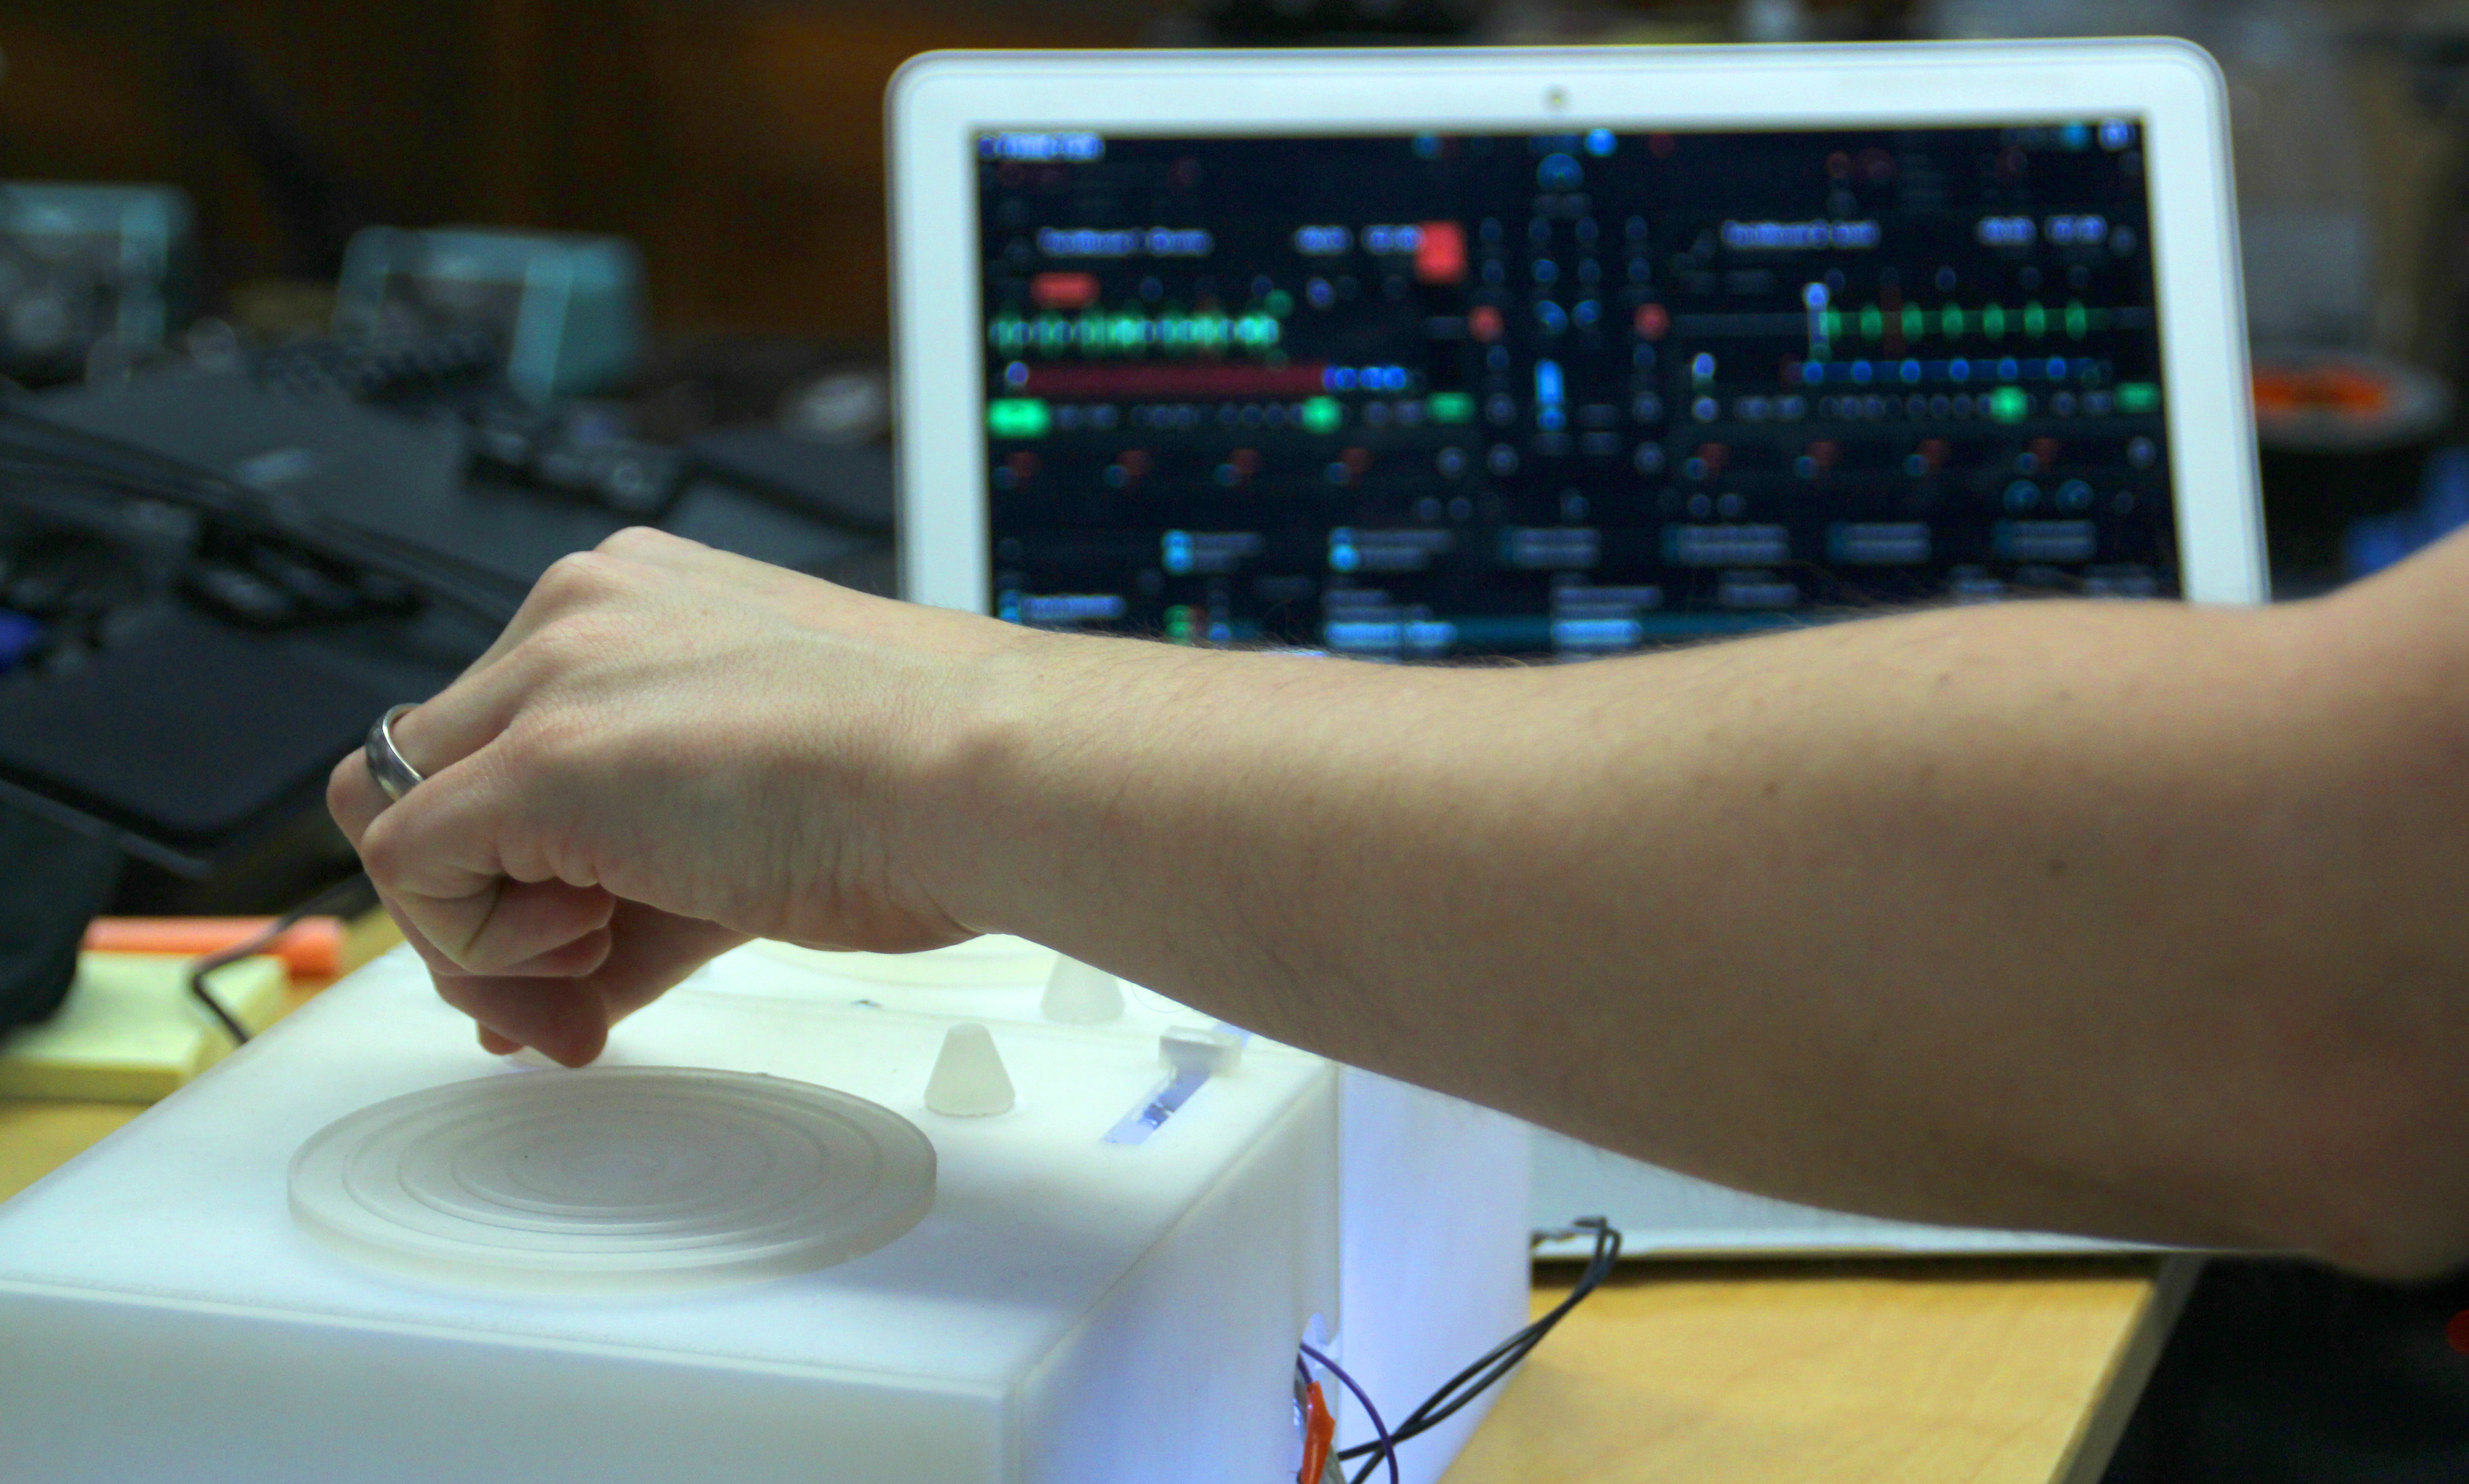
\includegraphics[width=3.25in]{figures/sauron/DJ-controller-action.JPG}
\caption{Our DJ mixing board, based on one of our users's designs, has sliders and two dial configurations: raised knobs for easy manipulation of volume, and a larger flat wheel for seeking and scratching songs.  The different types of dials share a sensing algorithm, however, as their interior parts are similar.}
\label{fig:sauron-djmixer}
\end{figure}
        
        \subsubsection{Game Controller}
        We developed two versions of a video game controller, shown in Figures \ref{fig:sauron-teaser} and \ref{fig:sauron-step-by-step}. To test responsiveness, we built a simple browser-based game to accept data from Sauron's WebSockets server. The controller moves the player character around (joystick) and shoots fireballs (buttons). We found the game was playable, although detection of the joystick position was noisy. This seems to be due to the fact that the blobs tracked for the main base and the two flanks were lumped together when the joystick was in certain configurations, e.g., at extreme right. We believe this is not a fundamental issue and could be mitigated by iterating on the joystick's interior design or by using a higher-resolution camera.

\section{Discussion}

Current Sauron prototypes are all tethered to a PC. There are opportunities to explore interactive devices not connected to computers. For example, tangible peripherals for mobile device could also be prototyped using our system. Modern smartphones have on board cameras and LED flashes, and enough on-board processing to perform computer vision. Modeling the phone and its camera parameters could enable mobile prototypes designed to encase the phone.

We believe that an exciting use for Sauron is in the development of entirely novel input devices which are not supported by traditional electronics. One example is a curved slider: electronics typically measure either linear or rotary motion, but a slider on a curved or irregular track would be easily prototyped using Sauron.

The creation of interactive prototypes also need not be limited to 3D printed plastic. Digital fabrication opens the doors to many new areas of exploration: any process which fabricates material according to a model created in software could be processed similarly. One such promising technology is laser cutting, where we already see the ability to create 3D models through sliceforms or layering of 2D cross-sections of an object. Laser Origami \cite{mueller-laserorigami} has pushed the bounds further, and it is not difficult to imagine fully laser-cuttable mechanisms that could be tracked by Sauron.

For future work we hope to test our tool more extensively with designers in the context of a workshop or class. We are also planning to explore tools to simplify the physical design process for users unfamiliar with CAD tools. 

    \subsection{Sweet Spots}
    
    Sauron works very well for prototyping the hand-feel and interactions of devices. It does not allow prototyping realistic weights, as it requires hollow models. Sauron also works best for roughly hand-sized devices (with our camera). Prototyping larger devices would be possible using a higher-resolution image device.
    
    \subsection{Limitations}
    
    We have identified several limitations of the Sauron system. Some are inherent to the approach, while others could be mitigated with additional engineering.
    
    \subsubsection{Post-print assembly}
    
    Currently, our prototypes still require some post-printing assembly for marking components and inserting mirrors. However, we believe this step is significantly less time-consuming than the process of wiring up a prototype with discrete electronic components. \valkyrie{we can show that this isn't always necessary}

    \subsubsection{Necessity of registering components post-print}
    A second limitation is the required registration process after printing. In future work we plan to create more sophisticated algorithms which can pre-determine bounding boxes of printed components using the digital model, or which can generate visual markers to denote end points and motion type. This would allow designers to skip the registration step.
    
    \subsubsection{Visible light does not work in all environments}
    Because we currently use visible light sensing, environmental lighting can interfere with our algorithms. For example, our prototypes behave erratically when tested with bright fluorescent lights directly overhead. Some components, like the slider and joystick, require a certain amount of clearance around them to move properly. When bright light shines through these gaps, vision tracking can become problematic. One remedy is to move sensing into the infrared spectrum.% though IR ., however this would preclude testing prototypes outdoors.\bjoern{visible light has the same problem.}
    
    \subsubsection{Model modifications do not chain}
    Our algorithms do not deal with cases where chaining of model modifications is required: i.e., if a component could be seen by first extruding, then reflecting, it will not be correctly processed by our algorithm. We provide the field of view of our camera as a reference to designers so that they can correct cases like this on their own, however more complex automatic interior geometry modifications are possible. 
    
    \subsubsection{Limited component library}
    Finally, we support only a limited library of components, and not all components can be modified through extrusions. However, this library is extensible by expert users who can define and label faces for extrusion and who can choose or program appropriate tracking algorithms. Our informal evaluation suggests though that configuring and changing existing components to suit the needs of a particular prototype may be sufficient to cover a useful design space.
\chapter{The Final Word}

\begin{quote}
When I look into the future, it's so bright it burns my eyes.

--- Oprah Winfrey
\end{quote}

This thesis has presented techniques for leveraging and modifying digital geometry of objects to aid in creating fast, cheap, and flexible prototyping tools. We conclude with a discussion of the links between and importance of described projects, as well as pointers to future work.

%\section{Restatement of Contributions}

%We presented a design space describing how to interlink geometry and sensing for digitally-fabricated prototype objects, as well as a series of explorations in promising areas of the design space. Specifically, we contributed:

%\begin{enumerate}
\item Fabbing to sense: a model and sensing co-design technique which uses knowledge of a particular sensing paradigm to automatically modify digital design files before fabrication, allowing improved or training-free sensing of the fabricated prototype. We offer three exemplars of this technique: Midas, Lamello, and Sauron.
\item Midas, a method for automatically generating custom capacitive touch sensors---cut from adhesive-backed conductive foil---by synthesizing sensor pads and routing connections from a high-level graphical specification:
%which allows a designer to author a high-level graphical specification of an object---and from that creates custom-shaped, flexible capacitive touch sensors by synthesizing sensor pads, auto-routing connections, and generating instructions for assembly and use: 
\begin{enumerate}
    \item a design tool using this method to enable users to to fabricate, program, and share touch-sensitive prototypes
    \item an evaluation demonstrating Midas’s expressivity and utility to designers
    \end{enumerate}
\item Lamello, a technique using passive plastic tine structures, 3D printed at interaction points and with predictable vibrational frequencies, to create passive tangible inputs sensed via audio:
%a technique which integrates algorithmically-generated audio-producing tine structures into movable components, creating passive tangible inputs---sensed by a microphone which classifies the tine-generated audio---that do not require training examples for accurate sensing:
\begin{enumerate}
    \item a design pipeline which predicts tine frequencies (and an evaluation that they can be accurately predicted) and senses user manipulation of components in real time
    \item a discussion of information encoding techniques useful for this technique, and a series of scripts to generate parts utilizing these encodings
    \end{enumerate}
\item Sauron, a design tool enabling users to rapidly turn 3D models of input devices into interactive 3D printed prototypes where a single camera senses input: %\valkyrie{this is the clearest description. modify others to be like this!}
\begin{enumerate}
    \item a method for tracking human input on physical components using a single camera placed inside a hollow object
    \item two algorithms for analyzing and modifying a 3D model’s internal geometry to increase the range of manipulations that can be detected by a single camera.
    \item an informal evaluation of our implementation of these techniques usable on models constructed in a professional CAD tool.
    \end{enumerate}
\end{enumerate}

\section{Discussion of Projects}

The large thrust of this thesis is this: designing tangible input devices is challenging---far more so than creating prototypes of graphical user interfaces---because prototypes must combine software, hardware, and custom enclosures. For this case, we believe digital fabrication can help. With digital fabrication, we have a model of an object \emph{before we have the object itself}, which we can manipulate and simulate in light of the sensing mechanism we plan to use for our final prototype. We call this process, which links fabrication-for-interaction to models-for-simulation, ``Fabbing to Sense."

The three projects we discussed---Midas, Lamello, and Sauron---serve as exemplars in exploring the space of Fabbing to Sense. Together, they leverage several of the most ``human'' senses: touch, hearing, and sight. As an illustration of the technique, this makes them accessible and easy to understand (though we also see opportunities in fabrication for senses for which humans have no direct analog, as with magnetic field sensors). Ultimately, designers and makers, and those that they create for, will not need to know the workings of the sensing mechanisms.

As with existing graphical user interface toolkits, which can abstract away callbacks, container structures, rendering styles, and other low-level details, we hope to see our techniques and others like them fade into the background; eventually they should be ignored in favor of designers' high-level goals, like ``button here," or ``continuous volume knob." We dipped into such high-level specifications in Midas, and found that designers were able to create unique input devices using the system.

Beyond simply supporting design tasks, we see simulation as a way to ensure that unusual sensing techniques can disappear from the perspective of users. Sauron, for example, performed simulations to ensure that its modifications would not interfere with users' manipulating input components through their full ranges of motion.

It may also be the designer's choice that the sensing mechanism \emph{not} fade into the background. In the Lamello project, we used sounds within typical human hearing ranges as control signals. While some may view this as a downside (and likely one that could be corrected using different materials and/or smaller structures), it is possible for designers to integrate this as a feature: as one example, a slider mechanism could be programmed to play a favorite song as it is manipulated. Thus, depending upon the selected modality, a designer may choose to either hide or accentuate a device's sensing technique.

In any case, integration of physical form-finding with specification of input components can be a challenge. This work is currently relegated to those with expertise in Computer-Aided Design (CAD) tools. While it does not fall under the banner of Fabbing to Sense, we have also done work on allowing users to create such physical specifications that are authored in the real world, using easily reconfigurable materials and leveraging computer analysis, simulation, and optimization \cite{savage-mmarks}. We see this as part of the future ecosystem of Fabbing to Sense.

All of the above is part of a larger trend in computer science, and especially in Human Computer Interaction, whereby computing devices are imbued with domain expertise, and further they are given the ability to assist users via guidance or corrective actions. This human-machine interlink can exploit the strengths of each system. That is, it marries human creativity and perceptive skills with machine precision and simulation. Systems connecting the two have been tested already for use in surgical (e.g., \cite{kahol-surgical}) and cooking (e.g., \cite{sato-mimicook}) environments, as well as innumerable other physical and virtual Augmented Reality (AR) environments for teaching novices or supporting experts. As more systems successfully demonstrate this technique, the human-machine interlink for aiding designers in their creation of tangible input devices represents a natural research direction, as well as a necessary component for designing the future of interaction.

\section{Future Work}

Over the course the thesis, we have pointed to a variety of limitations and possible improvements per-project. In general, we see open sourcing the projects and making their sensing apparatuses more mobile to be interesting engineering and research tasks. All three projects use sensing types common to today's mobile smart phones (capacitive touch, microphone-based audio, and camera-based video), and additional engineering could better leverage those and other sensors already available to designers from within their environment.

Beyond per-project improvements, we have laid out a design space for linking geometry to sensing. Midas, Lamello, and Sauron each represent a single point in this design space, and fuller exploration of the space may lead to companion projects to those described here. In particular, the advent of multi-material PolyJet 3D printers seems to open a wide variety of options for exploring colors, transparency, and flexibility as features in a sensing design space, and the Voxel8 \cite{voxel8} printer, which can lay arbitrary conductive materials and plastic together in a single pass, points to opportunities to explore induction, human body heat sensing, or magnetism as sensing operations. Or, as discussed in chapter 2, translucent tubing for use with liquids and level sensors.

Overall, we recognize that there are several assumptions made by the projects presented in this dissertation. Namely, our projects leverage a \emph{single fabrication machine} for creating \emph{one prototype} at a time, which is \emph{hand-optimized} by a designer and sensed by a \emph{single} sensor. We discuss possibilities opened by willfully subverting each of these assumptions in turn.

\subsection{Ecosystems of fabrication machines}

The projects described in this dissertation have largely focused on single fabrication machines working to create a finished prototype object. We also see opportunities for combining the abilities of several machines, whether to speed up the prototyping process or to investigate unique properties that allow exploration of the machines and sensors design space.

    \subsubsection{For celerity}

    While 3D printers allow for near-infinite flexibility in the forms that they are able to create, they still run very slowly. This can be compared to laser cutters, which offer significant speedups in exchange for only producing 2- or 2.5D prototypes (or limited 3D prototypes, see \cite{mueller-laserorigami}). Some prior work has investigated speeding up fabrication through integration of lasercut and 3D printed pieces \cite{beyer-platener}, or use of building blocks with 3D printed parts \cite{mueller-fabrickation}; however, these speedups do not make any use of their knowledge of the completed object post-fabrication. As demonstrated in the Lamello project, lasercut tines integrated with 3D printed bodies allow for faster fabrication with similar accuracy. However, having a designer hand-assemble highly complex input mechanisms fabricated on multiple machines may be prohibitive in terms of time spent: better would be using pre-fabrication simulations to make these devices (partially) self-assembling \cite{tibbits-self-assembly}. 

    \subsubsection{For properties}
    
    Speed is a factor worth considering, but by leveraging multiple machines designers can additionally access a larger variety of properties. Plastic can offer a sturdy base with configurable haptics \cite{torres-hapticprint}, while inkjet-printed circuitry can provide a slide-in base for electronics. Lasercut or cnc-milled wood may pair well with delicate paper to create shape-changing interfaces \cite{yao-pneui}. Leveraging multiple properties (potentially in combination with multiple sensors, as below) may allow for Fabbing to Sense a greater variety of devices. And in some cases, these multi-machine integrations could allow for output in addition to sensing \cite{yao-pneui}.

\subsection{Branching prototypes}

One important benefit of digital models of prototypes is that they become like code: they can be stored, shared, replicated, versioned, and unit-tested. Version-control website github \cite{github} in 2013 added a built-in viewer for STL files in user repositories on the site, offering a powerful tool for those who wished to version their physical designs. However, each design is hand-crafted by the designer. In the future, we would like to explore tools which can create likely \emph{spaces} of prototype designs given an initial seed from a designer, and which then allow testing multiple similar designs in parallel. This could follow prior work on understanding design spaces and how computers can support designer exploration, particularly through parametric modeling \cite{woodbury-designspace, woodbury-parametric}. Given the nature of the sensing performed by the toolkits presented, this type of small multiples testing should be as straightforward as attaching the sensing module to each new prototype.

\subsection{Machine-optimized prototype designs}

While describing a design space and smartly \emph{exploring} points in it to test in parallel could support a designer who has something in mind, another opportunity lies in automatic \emph{generation} of digital interfaces to suit particular people and/or tasks. This is similar in theory to Cogtool \cite{john-cogtool}---which allows designers of web applications to demonstrate tasks for their interfaces, then optimizes the interface to make completion of those tasks as quick as possible for end-users---, and Supple/Supple++ \cite{gajos-supple,gajos-supplepp}---which model users' motor and vision capabilities and automatically adapt their GUI to suit.

We believe that there is significant territory to be explored in modeling users' individual capabilities as relevant to tangible input devices, as well as understanding how to create optimal inputs devices suited to specific tasks.

    \subsubsection{To suit particular users}

    Individual users have wide-ranging abilities and preferences, especially when it comes to something as personal as the hands. In addition, mobility-impaired users may have special requirements for input devices. Traditional mass-produced input devices are designed to be comfortable for $95$\% of target users, however the advent of digital fabrication allows for one-off objects with no startup costs like those associated with tooling in traditional manufacturing. Thus, we can measure the capabilities of a single person (How large are Giorgia's hands? How far can Ethan bend his thumbs? How fast can Shiry pinch her fingers together?), and use our results to design for that person specifically. Such measurements might inform dimensions (e.g., overall size of an input device), locations (e.g., spacing between buttons), or even sensitivity (e.g., matched to user grip strength). This has seen a bit of exploration in the form of anatomical scanning for medical devices \cite{smakman-curatio}, but \emph{motion} is critical for interaction.

    \subsubsection{To suit particular tasks}
    
    Our lives contain a variety of general-purpose input devices, like the mice and keyboards that we find at our desks, or the video game controllers we use when we unwind. As described above, with digital fabrication machines we can imagine a future in which each input device is uniquely suited to a single task: we can ask questions about a task, and how a particular person approaches it (What abilities does Pat tend to use most when playing League of Legends? How often does Friedhelm scroll through documents while editing them, compared to insert/delete tasks?), and use these to inform the layout (e.g., more frequently-used functions close to dominant hand/fingers) or sensitivity (e.g., a lighter push will activate a time-critical function, versus a more substantial push necessary for an irreversible function) of input devices.
    
\subsection{Multi-sensor Units}

In the interest of reducing assembly time, all of our projects leverage a \emph{single} sensor in a single location. However, many commercially-available sensor bundles could offer additional types of data. For example, modern smartphones collect a wide array of sensors---e.g., microphone, camera, accelerometer, gyroscope, magnetometer---into a package that could easily be attached to a single point in a prototype; likewise, Texas Instruments' BLE SensorTag sports an ambient light sensor, humidity sensor, barometric pressure sensor, magnetometer, temperature sensor, and more \cite{ti-sensortag}. By leveraging multiple of these sensors in a single prototype, we can create objects which respond to multiple modalities of interaction: for example, supporting the design of objects which integrate squeezable soft components sensed using air pressure, yet can also determine their orientation in space using an accelerometer, allows designers greater flexibility in their process. Modelling potential interference between different sensor types may present an interesting problem here.

\section{Closing Remarks}

As computing moves off the desktop and into the world, we see designers exploring many varieties of input devices to suit new and specific tasks. These new physical devices necessitate a new kind of prototyping, that does not rely fully on \emph{virtual} software but which can help create functional \emph{physical} objects in a fast, cheap, and flexible way. This dissertation has described digital fabrication as a means of accomplishing this: by linking a digital design to a completed physical object, we can shorten the drudgery associated with each iteration cycle by offloading expertise---that previously would have been required of the designer---to her computer collaborator. We have presented three examples of this: Midas performed sensor routing and used this knowledge to pre-program its capacitive sensor microcontroller and ensure assembly correctness. Lamello used 3D geometry to predict tines' resonant frequencies for audio sensing. Sauron manipulated an object's digital model to ensure that a single camera would be able to sense all the components inside, as well as to keep pieces from colliding in the hands of an end-user. All three represent the paradigm of ``Fabbing to Sense," which employs knowledge of the sensing technique that will ultimately be used \emph{early} in the design process, and optimizing prototypes for that technique.

Our suite of tools, and the space that they explore, will hopefully empower designers to invent and hone designs for the future of interaction.
%\chapter{Conclusions \& Future Work}

% \appendix

\printbibliography

\end{document}